% !TEX TS–program = pdflatexmk

\documentclass[lucida,biblatex]{sp} % use if you have the Lucida LaTeX fonts
%\documentclass{sp}          % default: uses Times font
\usepackage{textcomp}
\usepackage{graphicx}
\usepackage{algorithm}
\usepackage{algpseudocode}
\usepackage{tikz}
\usepackage{tikz-dependency}
\usepackage{gb4e}
\usepackage{amssymb}
\usepackage{pifont}
\usepackage{tipa}
\usetikzlibrary{fit,positioning}
\usepackage{setspace}
\usepackage{color}
\usepackage{bbm}
\usepackage{enumitem}
\usepackage{mathrsfs}  
\usepackage{bbm}
\usepackage{relsize}


\addbibresource{references.bib}

\usepackage[utf8]{inputenc}

%\linespread{2}


%tables
\usepackage{tabularx}
\usepackage{array}
\usepackage{booktabs}
\usepackage{multirow}
\newcolumntype{L}[1]{>{\raggedright\let\newline\\\arraybackslash\hspace{0pt}}m{#1}}
\newcolumntype{C}[1]{>{\centering\let\newline\\\arraybackslash\hspace{0pt}}m{#1}}
\newcolumntype{R}[1]{>{\raggedleft\let\newline\\\arraybackslash\hspace{0pt}}m{#1}}
\newcommand{\possessivecite}[1]{\textciteauthor{#1}'s (\textciteyear{#1})}
\renewcommand{\exp}{\text{exp }}


\definecolor{PinkyPurple}{RGB}{178,0,178}
\newcommand{\jd}[1]{\textcolor{PinkyPurple}{\textbf{[jd: #1]}}}

\newcommand{\eref}[1]{(\ref{#1})}
\newcommand{\tableref}[1]{Table~\ref{#1}}
\newcommand{\figref}[1]{Figure~\ref{#1}}
\newcommand{\appref}[1]{Appendix~\ref{#1}}
\newcommand{\sectionref}[1]{Section~\ref{#1}}

\newcommand{\todo}[1]{}
\renewcommand{\todo}[1]{{\bf \color{red} (TODO: {#1})}}

\newcounter{excounter}

%=====================================================================
%========================= preamble material =========================

% Metadata for the PDF output. ASCII-only!
\pdfauthor{Sebastian Schuster and Judith Degen}
\pdftitle{A Computational Model of Listener Adaptation to Speaker Variation in Use of Uncertainty Expressions}
%\pdfkeywords{Full keyword list}

% Optional short title inside square brackets, for the running headers.
% If no short title is given, no title appears in the headers.
\title{I know what you're probably going to say: \\ Listener adaptation to variable use of uncertainty expressions}

% Optional short author inside square brackets, for the running headers.
% If no short author is given, no authors print in the headers.
\author{% As many authors as you like, each separated by \AND.
  \spauthor{Sebastian Schuster and Judith Degen\\ \today}
}

%=====================================================================

\begin{document}

%=====================================================================
%============================ frontmatter ============================

\maketitle

\begin{abstract}
\todo{Write me!}
\end{abstract}

%\begin{keywords}
%  Keywords (special formatting is fine)
%\end{keywords}

%=====================================================================
%============================ article text ===========================

\section{Introduction}


One of the key assumptions in Gricean pragmatic reasoning \citep{Grice1975} is that listeners reason about alternative utterances when interpreting a speaker's utterance. For example, consider the following sentences that give rise to scalar implicatures \citep{Horn1984}.

\begin{exe}
  \ex 
  \begin{xlist}
    \ex Alex: Bill ate some of the cookies.
    \ex \label{ex:cookie-inf} $\rightsquigarrow$ Bill did not eat all of the cookies.
  \end{xlist}
  \ex 
  \begin{xlist} 
    \ex Tom: The movie was ok.
    \ex \label{ex:movie-inf} $\rightsquigarrow$  The movie was not great.
  \end{xlist}
  \ex 
  \begin{xlist} 
    \ex Sue: It might snow tomorrow.
    \ex \label{ex:snow-inf} $\rightsquigarrow$  It is not certain that it will snow tomorrow.
  \end{xlist}
\end{exe}
According to Gricean pragmatic theories, listeners assume that a speaker is cooperative and arrive at the inference in (\ref{ex:cookie-inf}) through a counterfactual reasoning process: they reason that if Alex had wanted to communicate that Bill ate all of the cookies, Alex would have uttered the more informative statement \textit{Bill ate all of the cookies}. Assuming that Alex knew the truth regarding the more informative sentence, it must be that the more informative statement is not true, which leads the listener to conclude (\ref{ex:cookie-inf}). Analogous reasoning leads to the inferences in (\ref{ex:movie-inf})  and (\ref{ex:snow-inf}) .

An implicit assumption in such an account of pragmatic reasoning is that listeners have precise expectations about the speaker's language use in different situations -- listeners will only be able to draw correct pragmatic inferences if they know what a speaker would have said to communicate alternative world states. Arguably, this assumption is valid in many contexts -- after all, languages are highly conventional systems (\todo{Cite something??}) and different speakers  often agree on descriptions for different world states. However, for more abstract function words such as quantifiers like \textit{some} and \textit{many} or uncertainty expressions like \textit{might} and \textit{probably}, there exists more variability across speakers. For example, in a norming study, \citet{Yildirim2016} found that participants varied considerably in their expectations about the use of different quantifiers. Similarly, \citet{Wallsten1986} found considerable inter-subject variability in the interpretation of uncertainty expressions. 

Recent work suggests that listeners deal with this kind of variability by adapting to it and updating their expectations about a speaker's language use, a process known as semantic/pragmatic adaptation. In a series of experiments, \citet{Yildirim2016} exposed participants to different speakers whose use of the quantifiers \textit{some} and \textit{many} varied. After exposure, they probed participants' expectations about the speakers' language use and found that participants indeed formed speaker-specific expectations. However, while the results consistently suggest that listeners are updating \textit{some} type of expectations, the nature of the expectations that listeners are updating is unknown. 
In particular, it is still an open question whether this kind of semantic/pragmatic adaptation is a result of listeners learning speaker-specific utterance preferences or whether listeners form speaker-specific semantic representations. 
\jd{and why do we care about the nature of the expectation? be clearer already here about what the implications are for theories that assume static meanings}Answering this question is the focus of the work reported here.

As a starting point for this investigation, we consider adaptation in other linguistic domains. Apart from the work on quantifiers, linguistic adaptation has been observed in  phonetics \citep[e.g.,][]{Goldinger1998,Norris2003,Kraljic2005,Kraljic2007,Babel2012,Kleinschmidt2015}, 
syntax \citep{Kamide2012,Fine2013,Fine2016,Myslin2016,Kroczek2017},\footnote{Note, 
However, that some of these studies failed to replicate and it is still unclear under what 
circumstances syntactic adaptation can be observed \citep[see ][]{Liu2017,HarringtonStack2018}.} intonation and prosody \citep{Kurumada2012,Roettger2019}, and with phenomena such as referring expressions
\citep{Clark1986,Brennan1996,Metzing2003,Horton2005,Brennan2009} and lexical associations \citep{DelaneyBusch2019}. 

For most of these phenomena, there . \jd{this may be a little too strong?} At the phonetic level, 
listeners update their expectations about speakers' \textbf{mapping} between acoustic cues and phonemes \citep[e.g.,][]{Kleinschmidt2015}.
At the syntactic level, listeners update their expectations about speakers' \textbf{preferences} 
for different syntactic structures. In contrast, at the semantic/pragmatic level the adaptation process and the nature of the updated representations is still poorly understood. \jd{is semprag adaptation inherently a more difficult problem than phonetic and syntactic adaptation? if so, it's worth emphasizing here}

We investigate two likely candidates for representations that are updated during semantic/pragmatic adaptation, motivated by recent advances in probabilistic modeling of pragmatic language understanding \cite{FrankGoodman2012,GoodmanFrank2016,FrankeJaeger2016}. First -- analogous to phonetic adaptation -- listeners might update their beliefs about speakers' mappings between 
words and world states, i.e., speakers' lexica. Alternatively -- analogous to syntactic adaptation -- 
listeners might update their beliefs about speakers' preferences
for expressions. Finally, listeners might track both mappings and preferences.

To illustrate how different beliefs about lexica and utterance preferences can lead to different interpretations, consider the interpretation 
of the uncertainty expression \textit{probably} produced by three different hypothetical speakers. For the sake of this example, 
let us assume the only three expressions that a speaker can choose from are \textit{might}, \textit{probably}, and \textit{almost certainly}.
A listener's beliefs about the three speakers' lexica and preferences are schematically illustrated in Figure~\ref{fig:inference-example}.

\begin{figure}
\center
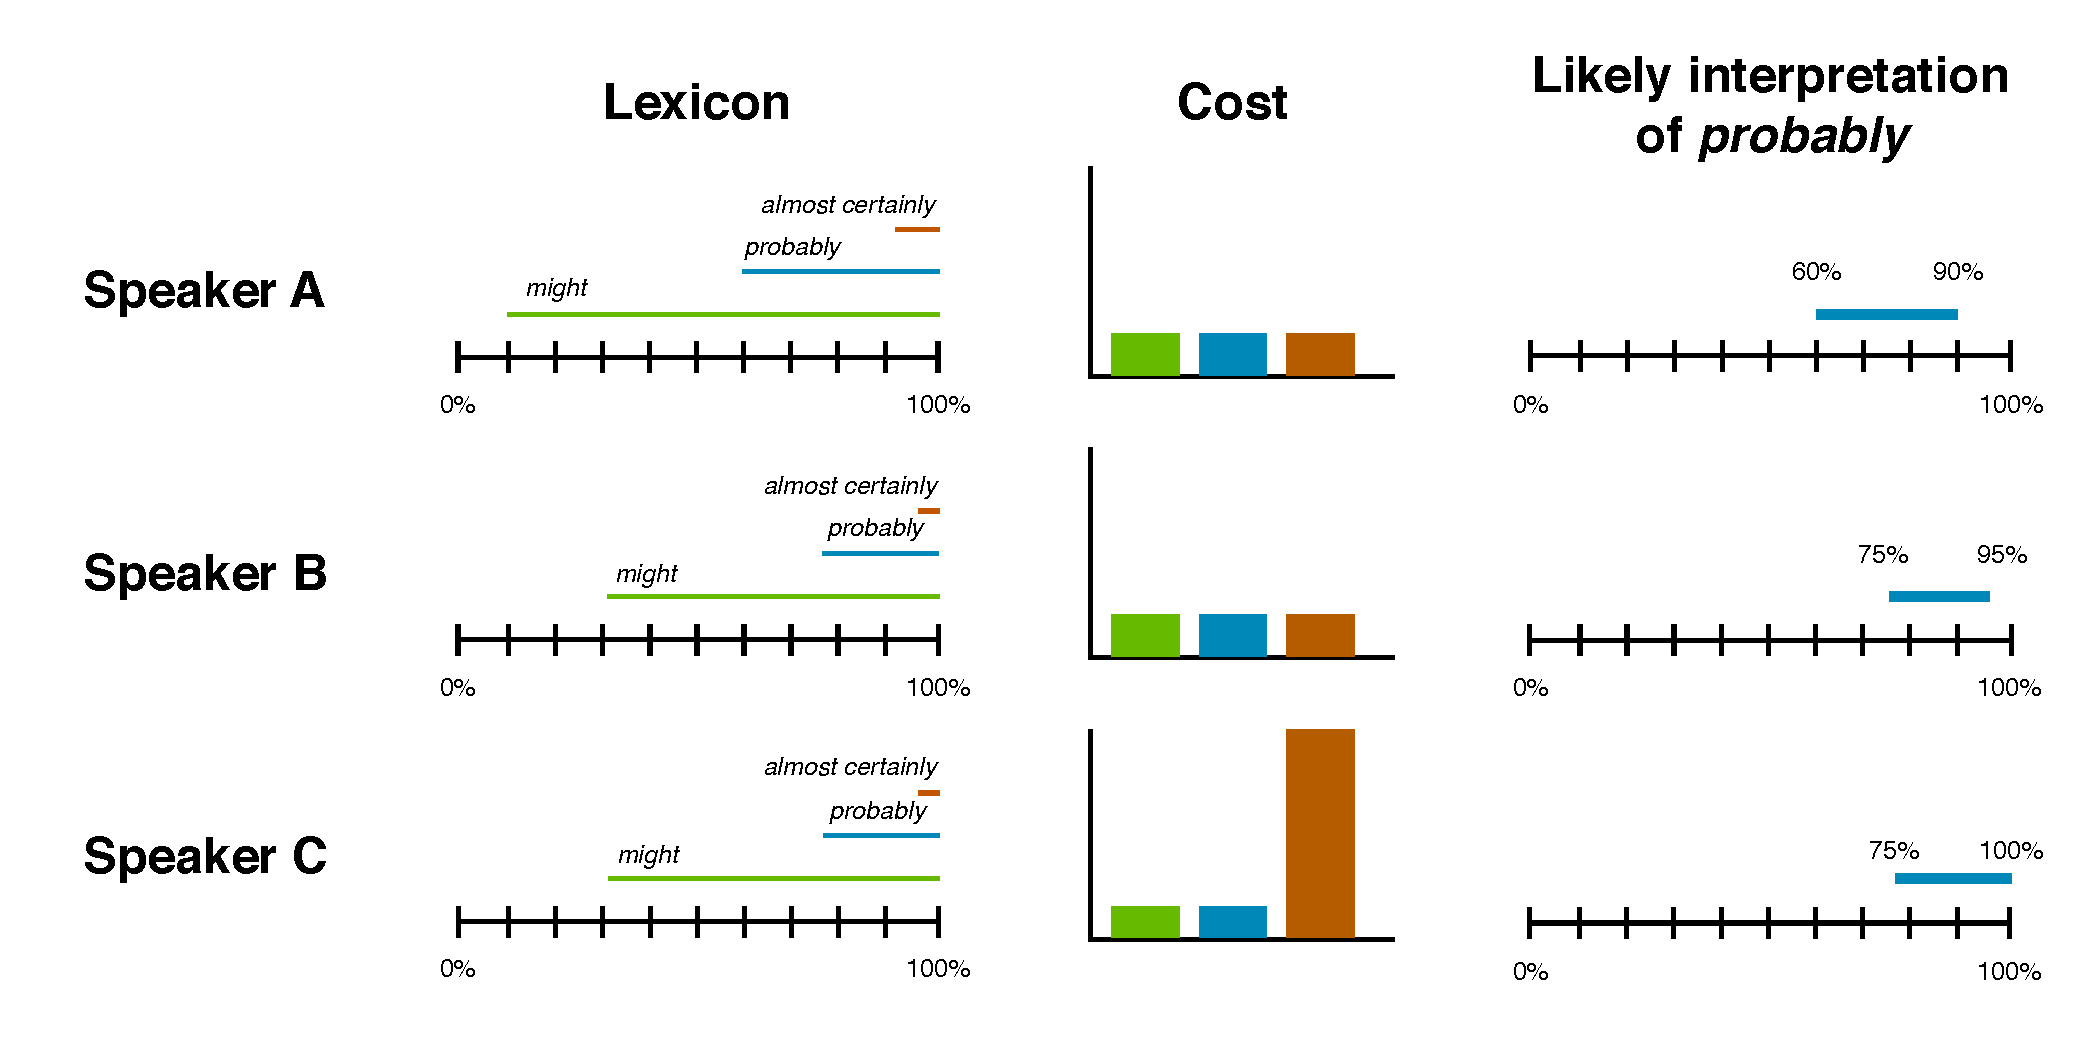
\includegraphics[width=\textwidth]{plots/implicatures.pdf}
\caption{Lexica, utterance preferences and likely interpretation of \textit{probably} for three different speakers. The region of the probability scale covered by each line in the Lexicon panel indicates the corresponding expression's literal semantics. Height of bars in the Preferences panel indicates the speaker's preference for each expression.    \jd{make sure that bar height here and bar height in the cost plots further into the paper mean the same thing. ie, if you're plotting cost later on, plot cost (dispreference) here as well}}
\label{fig:inference-example}
\end{figure}

First, consider speaker {\bf A}, for whom \textit{might} is semantically felicitous if the described event probability (e.g., of snowing) exceeds 10\%, 
\textit{probably} if the event probability exceeds 60\% and \textit{almost certainly}  if the event probability exceeds 90\%.  If a listener has accurate beliefs about {\bf A}'s mapping between expressions and event probabilities and observes {\bf A}  produce the sentence \emph{It will probably snow}, they will be likely to infer a probability of snowing between 60 and 90\%. As illustrated above, the reasoning follows the schema of a standard scalar implicature \citep{Grice1975, Horn1984}: if  {\bf A} had intended to communicate a probability above 90\%, they could have said \emph{It will almost certainly snow}, which would have been more informative and equally relevant. Assuming the speaker knows the actual event probability and is cooperative, it is therefore likely that the intended probability is not above 90\%.\footnote{Under a standard Gricean view, the negation of the stronger alternative is inferred categorically. However, we adopt probabilistic language here in keeping with recent results that scalar inferences are more aptly viewed as probabilistic inference under uncertainty.\jd{cite}} 

Now, consider speaker {\bf B}, for whom \textit{might} is semantically felicitous if the event probability exceeds 30\%, 
\textit{probably} if the event probability exceeds 75\% and \textit{almost certainly}  if the event probability exceeds 95\%. If a listener has
accurate beliefs about {\bf B}'s mappings, they will be likely to infer, via the same reasoning as above, a chance of snow between 75\% and 95\% when they hear {\bf B} produce the same sentence, \textit{It will probably snow}.

Finally, consider speaker {\bf C}. {\bf C} uses the same mapping between expressions and event probabilities as {\bf B}. However, {\bf C} has a strong preference against 
producing \textit{almost certainly}. If a listener has accurate beliefs about {\bf C}'s lexicon and production preferences, 
they will be likely to infer a chance of snow between 75\% and 100\% when they hear {\bf C} produce \textit{It will probably snow} since they will not
consider  \textit{almost certainly} a likely alternative. That is, the scalar inference will be blocked by the additional knowledge of the speaker's production preferences. 

Thus, a listener who tracks the variability in these hypothetical speakers' lexica and production preferences will draw on average more accurate inferences about the world. We investigate the nature of the representations updated during semantic/pragmatic adaptation in the the domain of uncertainty expressions, i.e., words or phrases that can be used to express uncertainty, as used in descriptions of potential future events. These expressions include epistemic modals such as \textit{might}, 
\textit{probably}, and \textit{could} (see, for example, \citep{Kratzer1991} and \citep{Hacquard2011}) but also phrases such as \textit{it looks like}, which have been primarily investigated in the experimental pragmatics literature (e.g., \cite{Kurumada2014,Pogue2018}).

Uncertainty expressions have several properties that make them a good testing ground for studying semantic and pragmatic
adaptation. First, there is no consistent mapping between uncertainty expressions and event probabilities
(see, for example, \citet{Clark1990}, \citet{PepperPrytulak1974}). \jd{is it worth problematizing more clearly the semantic assumption of invariance of meaning for these uncertainty expressions? take inspiration from dan's book?} Second, there is considerable inter-speaker variability 
in the use of these expressions \citep{Wallsten1986} and therefore it is likely that listeners expect different speakers to use these expressions
differently. Lastly, interpreting uncertainty expressions plays an important role in many everyday situations from the banal -- such as talking about the weather -- to the serious -- such as communicating about health risks \citep{Berry2004, Lipkus2007, Politi2007} or making financial decisions \citep{Doupnik2003}. 
Thus, listeners would benefit from tracking  how a given speaker uses these expressions. %and are therefore  potentially more attuned to subtle differences across speakers than in cases where variation may have a smaller effect on decision-making.

In order to establish the nature of the representations that are updated during adaptation to variable use of uncertainty expressions we proceed through the following steps:
\begin{enumerate}
	\item Quantify the variability in listeners' expectations about a generic speaker's production of uncertainty expressions (\sectionref{sec:exp-norming}).
	\item Propose a probabilistic computational pragmatics model of the production of uncertainty expressions that functions as proxy for listeners' baseline generative model of a generic speaker. Evaluate the model on the data from Experiment 1. (\sectionref{sec:model-baseline}).
	\item Measure whether and to what extent listeners update their expectations when exposed to a speaker who is either more cautious or more confident in their use of uncertainty expressions than the baseline speaker model (Experiment 2, \sectionref{sec:exp-prod-adaptation}).
	\item Create three versions of the baseline model which differ  in terms of which model components are updated in response to exposure to simulated cautious and confident speakers: update on only production preferences, only the lexicon, or both. Use model comparison between these three adaptation models as a hypothesis-testing tool to infer which representations undergo adaptation, by evaluating which adaptation model best captures the observed post-exposure expectation data from Experiment 2 (\sectionref{sec:model-adapt}).
	\item To further test the adaptation models, use them to derive predictions about post-exposure interpretation. Measure interpretation and evaluate the model (Experiment 3, \sectionref{sec:exp-model-interpretation}).
\end{enumerate}


%The rest of this paper is structured as follows. In the next section, we present results from a norming study that show that listeners vary in their
%expectations of what uncertainty expressions a generic speaker will use to describe different event probabilities. 
%In section~3, we present a game-theoretic computational model of listeners expectations about a generic speaker's use of uncertainty expressions.
%In section~4, we present an experiment that provides evidence for listener's updating their expectations after brief exposure to different speakers.
%In section~5, we present our adaptation model and argue based on model simulations that listeners are updating their expectations about preferences and
%lexica.
%In section~6, we discuss how our model also predicts updated interpretations of uncertainty expressions after a brief exposure to a different speaker and 
%we present an experiment whose results confirm this prediction. 

We find that listeners indeed update their beliefs about different  speakers' use of uncertainty expressions, and that this adaptation is reflected both in post-exposure measures of production expectations and interpretation. The data are best captured by the adaptation model in which both the lexicon and the speaker's production preferences are updated. We conclude with a discussion of remaining open questions and the implications of our findings. \jd{implications for what? maybe at least mention here the theories of adaptation that already exist? also mention somewhere that the computational model is formulated within ``the Rational Speech Act framework, a state-of-the-art probabilistic formalization of the Gricean program'' and that this is one of the first extensions of the model to model learning}


%%%%%%%%%%%%%
% BEGIN OLD INTRO  %

%Coming home from work, you wonder whether it will finally snow tomorrow. As you step out of the car, your neighbor calls over the fence, \emph{``The weather app says it \textbf{might} snow tomorrow.''}  You nod and enter the house, and your partner calls from the kitchen,  \emph{``The weather app says it will \textbf{probably}  snow tomorrow.''} You know that your neighbor and your partner use the same weather app. As a listener trying to infer how likely it is that it will snow tomorrow, you now face the challenge that different speakers described the same event probability using uncertainty expressions that differ in strength -- \textit{probably} is conventionally a stronger alternative to \textit{might}. You might conclude from this variable linguistic evidence that one of them is lying. But you happen to know that your neighbor is relatively cautious in what they're willing to assert; your partner is much more confident. When you consult the weather app yourself, you are therefore not surprised to find that the probability of snow  is estimated at 60\%.
%
%
%As this example highlights, a listener who is faced with variability in language use 
%will be able to more accurately infer the world state that a speaker intended to communicate 
%if they track individual speakers' language use -- e.g., speakers' idiosyncratic lexical preferences or their idiosyncratic form-to-meaning mappings -- and form speaker-specific expectations about said speakers' language use, a process known as \emph{adaptation}. %That is, listeners can estimate generative models of a speaker and use this generative speaker model both to predict the speaker's likely utterances in different contexts and to infer the world state that specific speakers intend to communicate.
%
%Tracking of speaker-specific statistics and expectation adaptation has been observed in many linguistic domains, including phonetics 
%\citep[e.g.,][]{Goldinger1998,Norris2003,Kraljic2005,Kraljic2007,Babel2012,Kleinschmidt2015}, 
%syntax \citep{Kamide2012,Fine2013,Fine2016,Myslin2016,Kroczek2017},\footnote{Note, 
%However, that some of these studies failed to replicate and it is still unclear under what 
%circumstances syntactic adaptation can be observed \citep[see ][]{Liu2017,HarringtonStack2018}.} semantics and pragmatics \citep{Yildirim2016, Wittenberg2016}, intonation and prosody \citep{Kurumada2012,Roettger2019}, and with phenomena such as referring expressions
%\citep{Clark1986,Brennan1996,Metzing2003,Horton2005,Brennan2009} and 
%lexical associations \citep{DelaneyBusch2019}. 
%
%
%
%What is the nature of the expectations that listeners are updating? At the phonetic level, 
%listeners update their expectations about speakers' \textbf{associations} \jd{`association' is a weird word here. why use it? the point is that they update their beliefs about the distributions of various acoustic cues generated by a phoneme, no?} between acoustic cues and phonemes \citep[e.g.,][]{Kleinschmidt2015}.
%At the syntactic level, listeners update their expectations about speakers' \textbf{preferences} 
%for different syntactic structures.  At the semantic/pragmatic level, However, the adaptation process is still poorly understood: while the results by \cite{Yildirim2016}, discussed in more detail below, suggest that listeners update
%\textit{some} expectations about specific speakers' language use, 
%it is an open question what the nature of the representations is that are updated during semantic/pragmatic adaptation. 
%Answering this question is the focus of the work reported here.

%We  investigate two likely candidates for representations that are updated during semantic/pragmatic adaptation, motivated by recent advances in probabilistic modeling of pragmatic language understanding \cite{FrankGoodman2012,GoodmanFrank2016,FrankeJaeger2016}. First -- analogous to phonetic adaptation -- listeners might update their beliefs about speakers' associations \jd{need to think of better word and way to describe this functionally} between 
%words and world states, i.e., speakers' lexicon. Alternatively -- analogous to syntactic adaptation -- 
%listeners might update their beliefs about speakers' preferences
%for expressions. Finally, listeners might track both associations and preferences.


%To illustrate how different beliefs about lexica and utterance preferences can lead to different interpretations, consider the interpretation 
%of the uncertainty expression \textit{probably} produced by three different hypothetical speakers. For the sake of this example, 
%let us assume the only three expressions that a speaker can choose from are \textit{might}, \textit{probably}, and \textit{almost certainly}.
%A listener's beliefs about the three speakers' lexica and preferences are schematically illustrated in Figure~\ref{fig:inference-example}.
%
%\begin{figure}
%\center
%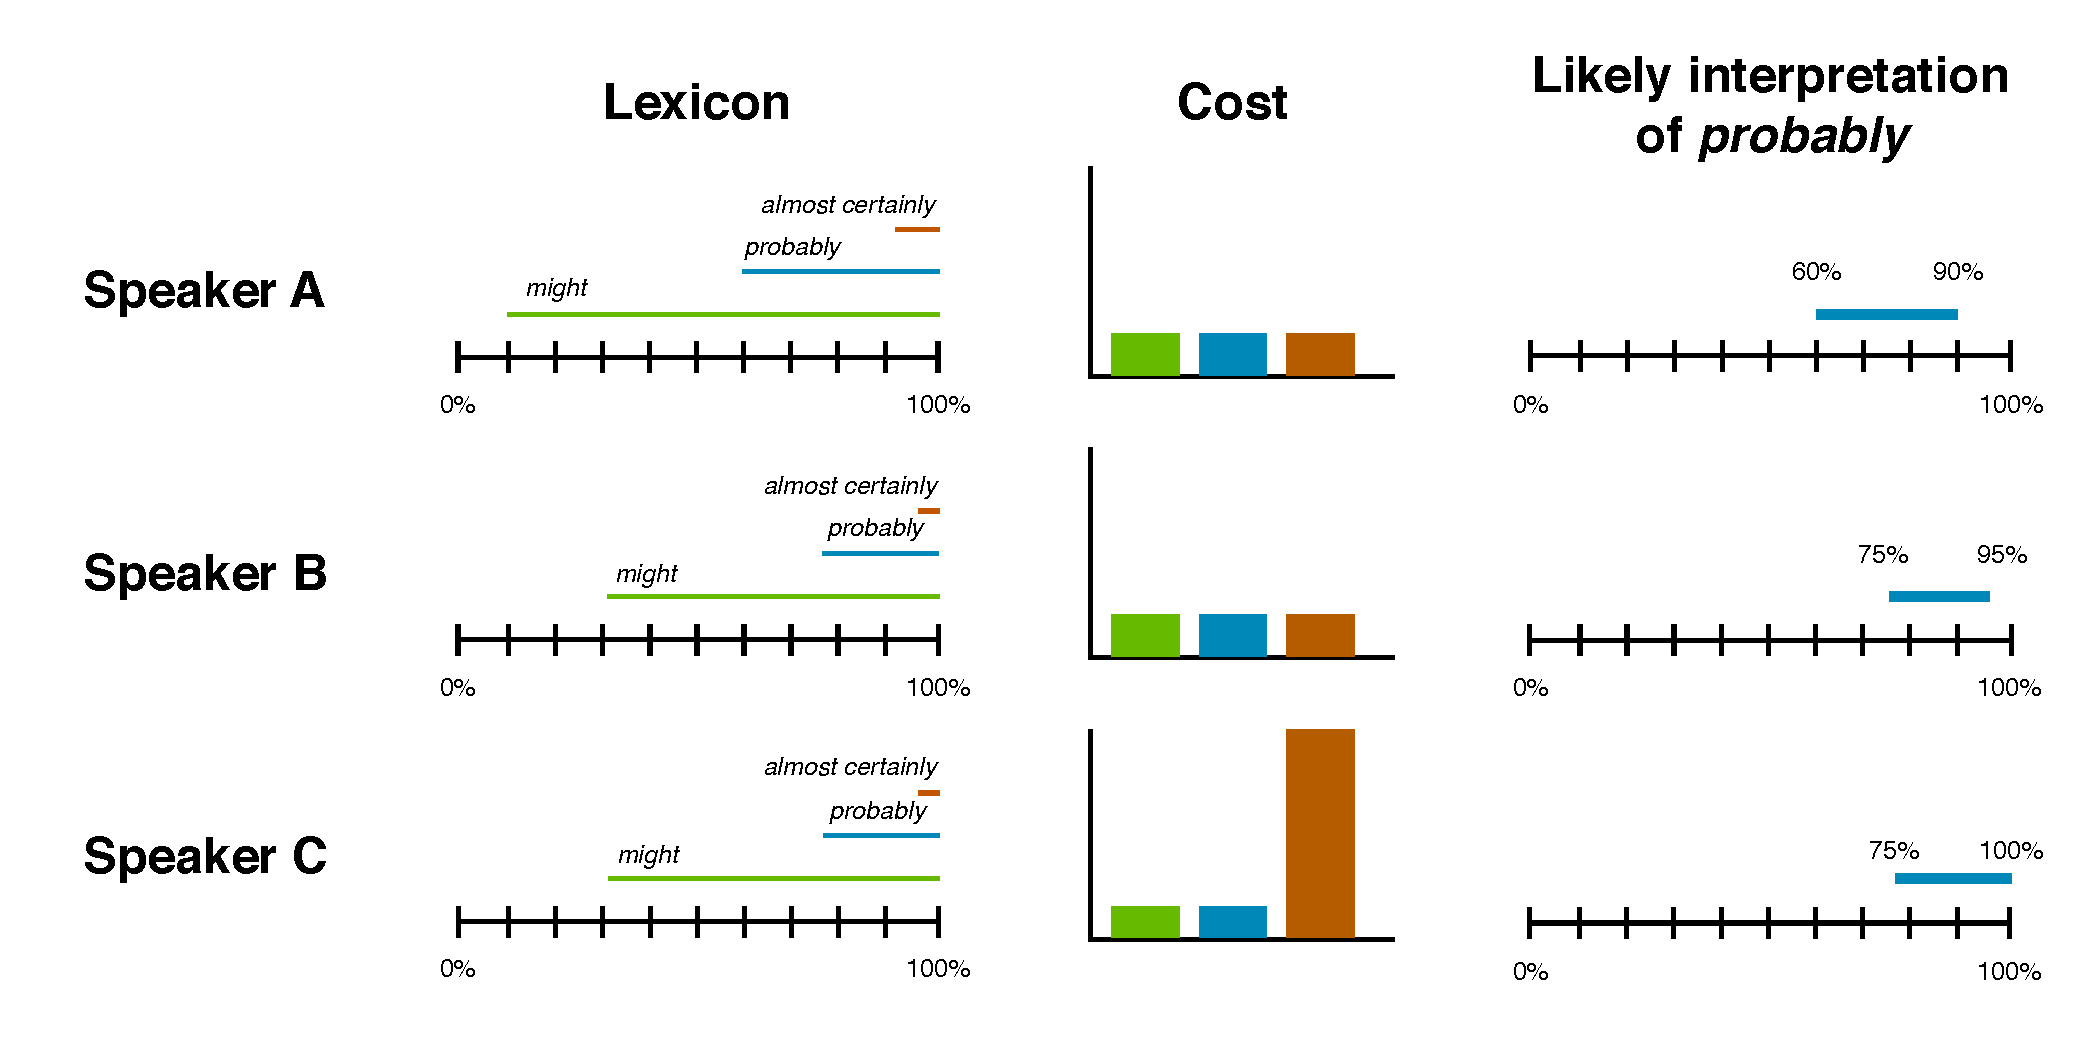
\includegraphics[width=\textwidth]{plots/implicatures.pdf}
%\caption{Lexica, utterance preferences and likely interpretation of \textit{probably} for three different speakers. The region of the probability scale covered by each line in the Lexicon panel indicates the corresponding expression's literal semantics. Height of bars in the Preferences panel indicates the speaker's preference for each expression.    \jd{make sure that bar height here and bar height in the cost plots further into the paper mean the same thing. ie, if you're plotting cost later on, plot cost (dispreference) here as well}}
%\label{fig:inference-example}
%\end{figure}
%
%First, consider speaker {\bf A}, for whom \textit{might} is semantically felicitous if the described event probability (e.g., of snowing) exceeds 10\%, 
%\textit{probably} if the event probability exceeds 60\% and \textit{almost certainly}  if the event probability exceeds 90\%.  If a listener has accurate beliefs about {\bf A}'s mapping between expressions and event probabilities and observes {\bf A}  produce the sentence \emph{It will probably snow}, they will be likely to infer a probability of snowing between 60 and 90\%. The reasoning follows the schema of a standard scalar implicature \citep{Grice1975, Horn1984}: if  {\bf A} had intended to communicate a probability above 90\%, they could have said \emph{It will almost certainly snow}, which would have been more informative and equally relevant. Assuming the speaker knows the actual event probability and is cooperative, it is therefore likely that the intended probability is not above 90\%.\footnote{Under a standard Gricean view, the negation of the stronger alternative is inferred categorically. However, we adopt probabilistic language here in keeping with recent results that scalar inferences are more aptly viewed as probabilistic inference under uncertainty.} 
%
%Now, consider speaker {\bf B}, for whom \textit{might} is semantically felicitous if the event probability exceeds 30\%, 
%\textit{probably} if the event probability exceeds 75\% and \textit{almost certainly}  if the event probability exceeds 95\%. If a listener has
%accurate beliefs about {\bf B}'s mappings, they will be likely to infer, via the same reasoning as above, a chance of snow between 75\% and 95\% when they hear {\bf B} produce the same sentence, \textit{It will probably snow}.
%
%Finally, consider speaker {\bf C}. {\bf C} uses the same mapping between expressions and event probabilities as {\bf B}. However, {\bf C} has a strong preference against 
%producing \textit{almost certainly}. If a listener has accurate beliefs about {\bf C}'s lexicon and production preferences, 
%they will be likely to infer a chance of snow between 75\% and 100\% when they hear {\bf C} produce \textit{It will probably snow} since they will not
%consider  \textit{almost certainly} a likely alternative. That is, the scalar inference will be blocked by the additional knowledge of the speaker's production preferences. 
%
%
%

%Thus, a listener who tracks the variability in these hypothetical speakers' lexica and production preferences will draw on average more accurate inferences about the world. We investigate the nature of the representations updated during semantic/pragmatic adaptation in the the domain of uncertainty expressions, i.e., words or phrases that can be used to express uncertainty, as used in descriptions of potential future events. These expressions include epistemic modals (see, for example, \citep{Kratzer1991} and \citep{Hacquard2011}) such as \textit{might}, 
%\textit{probably}, and \textit{could} but also phrases such as \textit{it looks like} which have been primarily investigated in the experimental pragmatics literature (e.g., \cite{Kurumada2014,Pogue2018}).
%
%Uncertainty expressions have several properties that make them a good testing ground for studying semantic and pragmatic
%adaptation. First, there is no direct mapping between uncertainty expressions and a speaker's belief about the likelihood of future events 
%(see, for example, \citet{Clark1990}, \citet{PepperPrytulak1974}). \jd{what does this mean?} Second, there is considerable inter-speaker variability 
%in the use of these expressions \citep{Wallsten1986} and therefore it is likely that listeners expect different speakers to use these expressions
%differently. Lastly, interpreting uncertainty expressions plays an important role in many everyday situations from the banal -- such as talking about the weather -- to the serious -- such as communicating about health risks \citep{Berry2004, Lipkus2007, Politi2007} or making financial decisions \citep{Doupnik2003}. 
%Thus, listeners would benefit from tracking  how a given speaker uses these expressions. %and are therefore  potentially more attuned to subtle differences across speakers than in cases where variation may have a smaller effect on decision-making.
%
%In order to establish the nature of the representations that are updated during adaptation to variable use of uncertainty expressions we proceed through the following steps:
%\begin{enumerate}
%	\item Quantify the variability in listeners' expectations about a generic speaker's production of uncertainty expressions (Experiment 1, \sectionref{sec:exp-norming}).
%	\item Propose a probabilistic computational pragmatics model of the production of uncertainty expressions that functions as proxy for listeners' baseline generative model of a generic speaker. Evaluate the model on the data from Experiment 1. (\sectionref{sec:model-baseline}).
%	\item Measure whether and to what extent listeners update their expectations when exposed to a speaker who is either more cautious or more confident in their use of uncertainty expressions than the baseline speaker model (Experiment 2, \sectionref{sec:exp-prod-adaptation}).
%	\item Create three versions of the baseline model which differ  in terms of which model components are updated in response to exposure to simulated cautious and confident speakers: update on only production preferences, only the lexicon, or both. Use model comparison between these three adaptation models as a hypothesis-testing tool to infer which representations undergo adaptation, by evaluating which adaptation model best captures the observed post-exposure expectation data from Experiment 2 (\sectionref{sec:model-adapt}).
%	\item To further test the adaptation models, use them to derive predictions about post-exposure interpretation. Measure interpretation and evaluate the model (Experiment 3, \sectionref{sec:exp-model-interpretation}).
%\end{enumerate}

%We find that listeners indeed update their beliefs about more cautious and more confident speakers' use of uncertainty expressions, and that this adaptation is reflected both in post-exposure measures of production expectations and interpretation. The data are best captured by the adaptation model in which both the lexicon and the speaker's production preferences are updated. We conclude with a discussion of remaining open questions and the implications of our findings.

%%%%%%%%%%%%%%%%%
% END ORIGINAL INTRO %%%%
%%%%%%%%%%%%%%%%%

\section{Pre-exposure ratings}
\label{sec:exp-norming}

We first conducted a series of norming studies, which served the following theoretical and methodological purposes.
First, they addressed the theoretical question of whether listeners vary in their expectations about
a generic speaker's use of uncertainty expressions, by collecting participants' judgments about expressions of uncertainty they expected speakers to use for varying probabilities of receiving gumballs of a particular color from a gumball machine. 
Second, they served as a methodological check on whether the paradigm is suited for manipulating fine-grained event probabilities. Third,  the results from these studies informed the experimental design of the adaptation experiments reported in later sections, by allowing us to both choose which pair of expressions of uncertainty to test adaptation on, and to determine the particular event probability for which participants had roughly equi-probable expectations about which expression of uncertainty a generic speaker would use to report an event with that probability. 
Lastly, we used the data collected in the norming studies to 
estimate population-level prior beliefs for the adaptation model reported in Section 5.

\subsection{Participants}
We recruited a total of 420 participants 
(20 per condition) on Amazon Mechanical Turk. 
We required participants to have a US-based IP address and a minimal approval rating of 95\%.
Participants were paid \$1.80 (condition 1), \$1.50 (conditions 2-15),
or \$2.00 (conditions 16-21),
%; condition 6a), 
depending on the number of trials,
which amounted to an hourly wage of approximately \$12--\$15. 

\begin{figure}
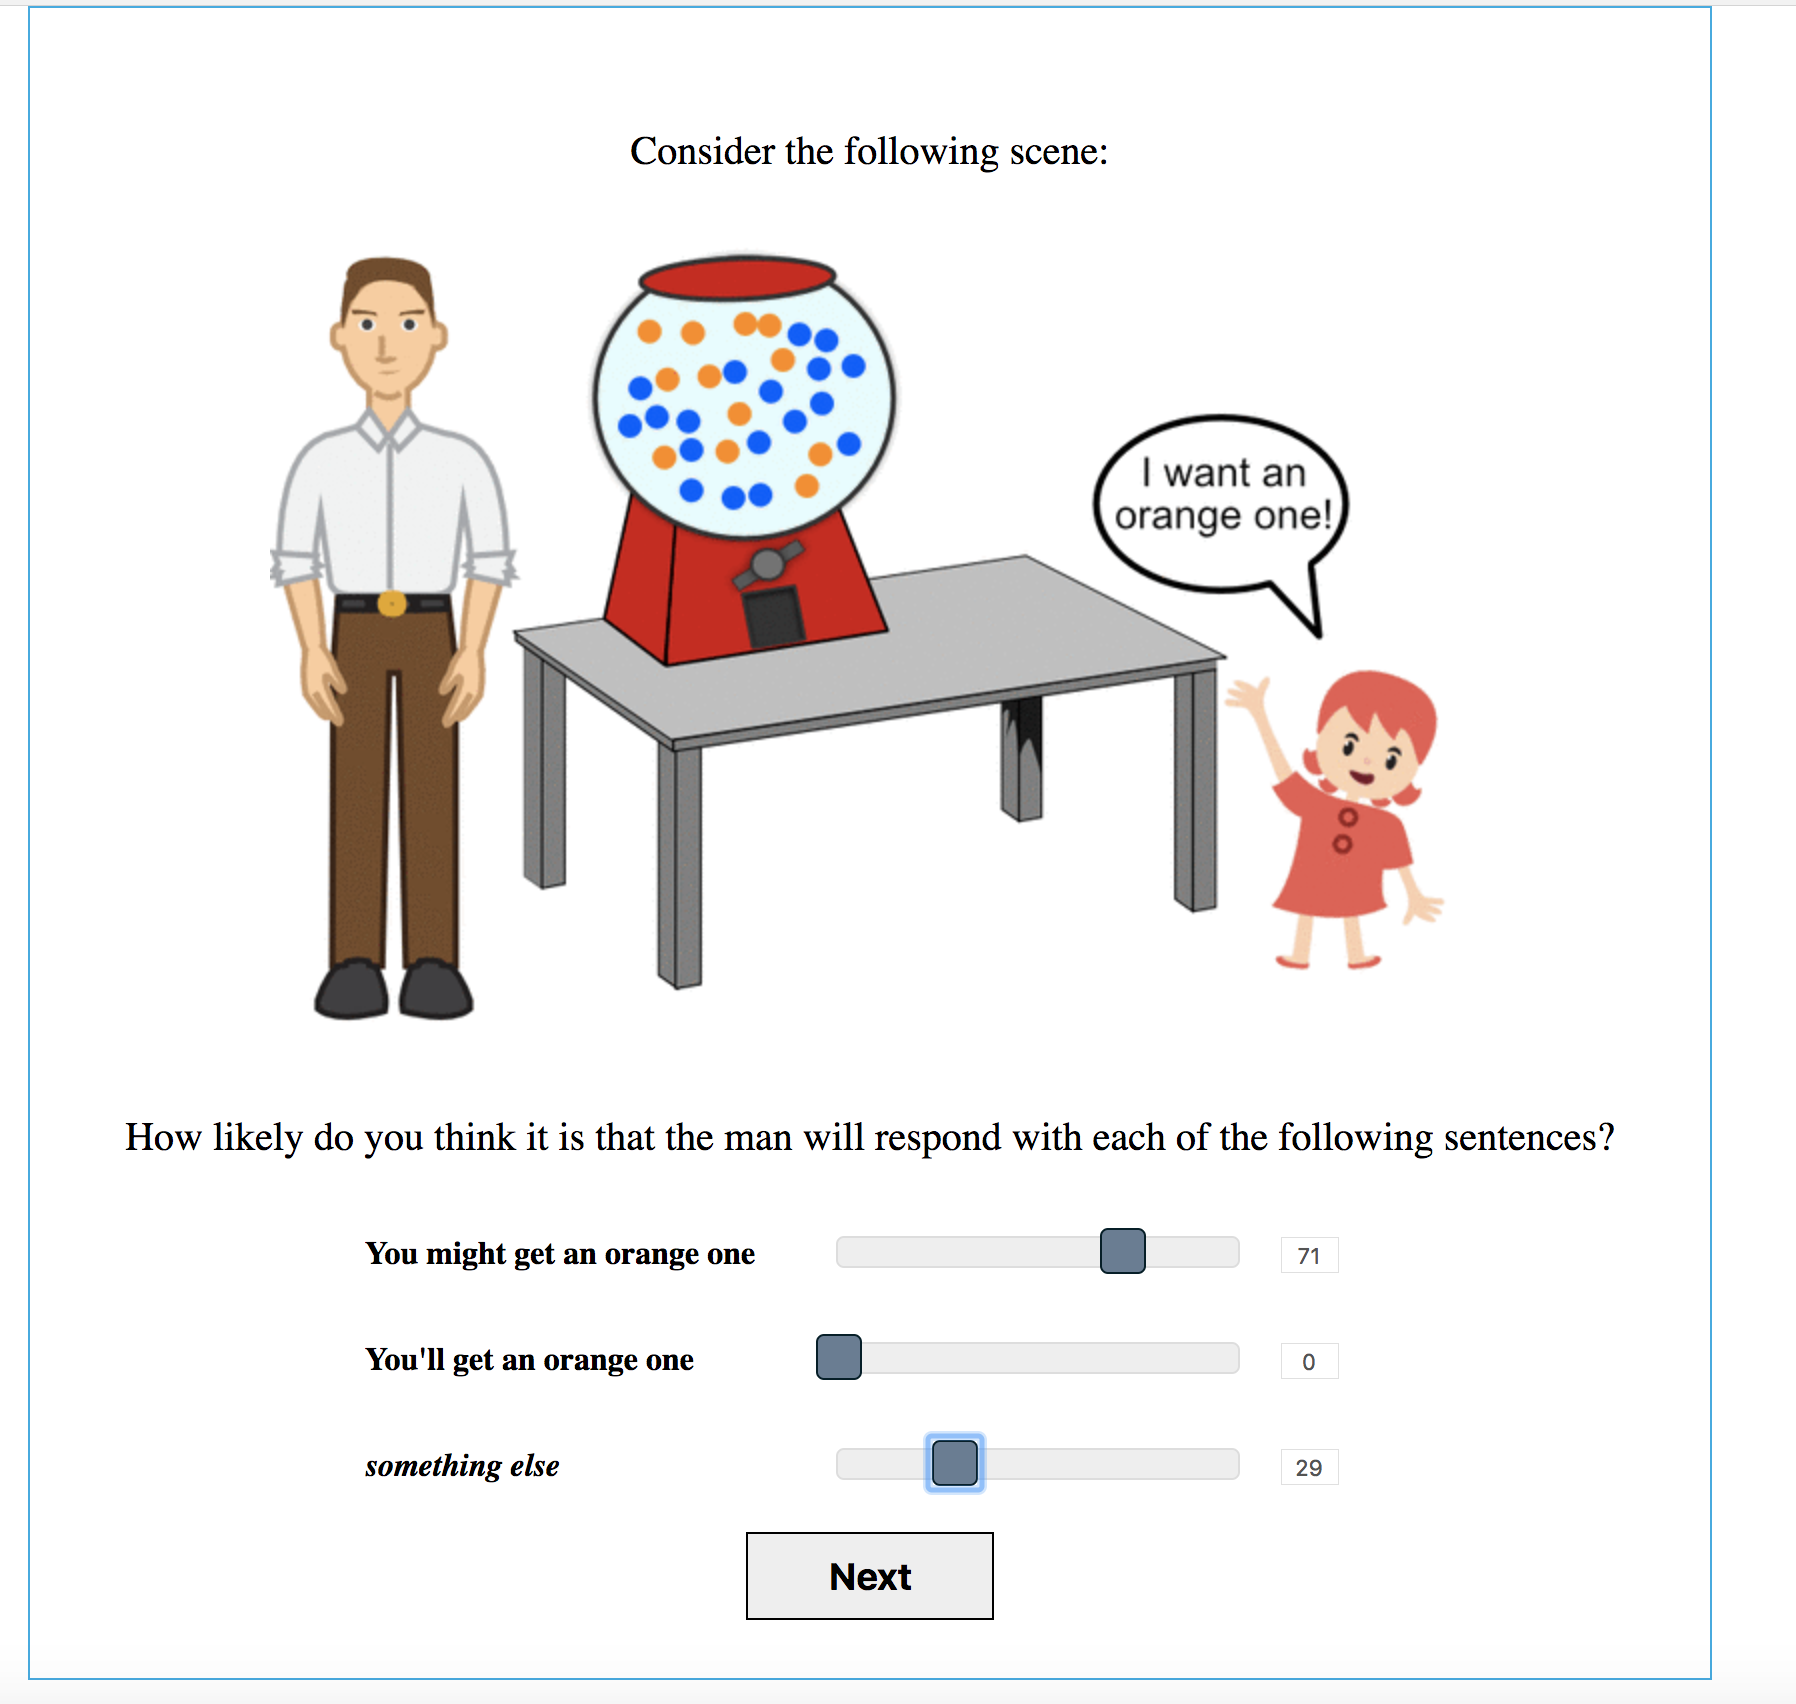
\includegraphics[width=\textwidth, trim={0 0 1.1cm 0},clip]{plots/pre-test-example-trial.png} 
\caption{Example trial from norming study. \label{fig:norming-trial} }
\end{figure}

\subsection{Materials and Procedure}
The norming study was a forced-choice production experiment. Participants were instructed 
that over the course of the experiment, they would see several scenes with an adult man, 
a young girl, and a gumball machine on a table and 
that the gumball machine is too high up on the table for the girl to see (see Figure~\ref{fig:norming-trial} for an example scene). 
After completing an attention check which asked participants whether 
the girl could see the gumball machine,\footnote{Participants had to go back to the instructions in case they responded incorrectly. This was the case for 41 participants.} 
participants saw a series of scenes  and were asked to rate how likely they thought it was that the 
adult would produce two given responses by distributing 100 points across the two given utterances and the 
blanket \textit{something else} option (\textsc{other}). Sliders automatically jumped back if participants tried to distribute more than 100 points. 
In each scene, the child uttered \textit{``I want a blue one''} (target color: blue) or  \textit{``I want an orange one''} (target color: orange), randomized across participants\footnote{In condition 1 (\textit{bare-might}), as well as conditions 16-21 (all conditions with \textit{bare not}), the target color was randomized across trials. While randomization of the target color across trials increased the correlation between the ratings for the two colors,  the average ratings for each condition independent of the target color were not affected by this choice. See the supplementary material for a detailed discussion of the effect of this manipulation on the ratings.}. The gumballs in the machines were tossed around continuously to prevent participants from counting the gumballs
and to make sure that participants did not consider it more likely to get one of the gumballs at the bottom of the machine.
 In each of the 21 conditions, participants saw only  two of the following seven possible adult utterances with different uncertainty expressions:

 \begin{itemize}
\item You'll get a blue/orange one. (\textsc{bare}\footnote{As a notational convention, we refer to utterances with uncertainty expressions in \textsc{small caps} and to the uncertainty expression itself in \textit{italics}. })
\item You might get a blue/orange one. (\textsc{might})
\item You'll probably get a blue/orange one. (\textsc{probably})
\item I think you'll get a blue/orange one. (\textsc{think})
\item It looks like you'll get a blue/orange one. (\textsc{looks like})
\item You could get a blue/orange one. (\textsc{could})
\item You won't get a blue/orange one. (\textsc{bare not})
\end{itemize}


\noindent Within each condition, we manipulated the percentage of target color gumballs across trials, which we take as proxy for the objective probability of receiving a gumball of the target color. 
Each participant saw 3 trials\footnote{In condition 1 (\textit{bare-might}), participants saw each gumball machine 6 times -- 3 times when being asked to produce a statement about orange gumballs and 3 times when being asked to produce a statement about blue gumballs. In conditions 15-20 (all conditions with \textit{bare not}), participants saw each machine 4 times: 2 times for each color.} 
for each of the following percentages: 0\%, 10\%, 25\%, 40\%, 50\%, 60\%, 75\%, 90\%, 100\%. We randomized the order of expressions across participants and trials were presented in pseudo-randomized order. \jd{pseudo-randomized how?}


\subsubsection{Results and Discussion}

\begin{figure}
\includegraphics[width=\textwidth]{plots/pre\string_test\string_main.pdf} 
\caption{Results from 3 conditions of the norming study. Error bars correspond to bootstrapped 95\%-confidence intervals. \label{fig:norming-results-main} }
\end{figure}

Figure~\ref{fig:norming-results-main} shows participants' ratings for different gumball proportions for 3 of the 21 conditions, namely all combinations of the conditions
with the utterances \textsc{bare}, \textsc{probably}, and \textsc{might} (see the Supplementary Material for the results from the other 18 conditions). 
The results from these three conditions highlight several important properties of participants'
behavior in this experiment that generalize to all conditions.
First, the ratings for individual utterances are influenced by the utterance choices presented to participants.
If we compare the ratings for \textsc{might} in the \textit{bare-might} and the \textit{might-probably} condition, we see that \textsc{might} received high ratings for a larger
range of event probabilities when it is paired with \textsc{bare} than when it is paired with \textsc{probably}. We observe similar effects for the other two utterances.
This suggests that participants are primed to use the utterances provided in the experiment and that their ratings depend on the presented alternatives -- an effect that
has also been observed for quantifiers \citep{DegenTanenhaus2015}.

Second, the results suggest that participants are sensitive to the different event probabilities and that this paradigm is well suited to study 
the mapping between event probabilities and uncertainty expressions. For example, in the \textit{might-probably} condition, participants
provided considerably different ratings when they were presented with a gumball machine with 50\% target color gumballs than when they
were presented with 60\% target color gumballs.

\begin{figure}
\includegraphics[width=\textwidth]{plots/pre\string_test\string_main\string_indiv.pdf}
\caption{Results of three individual participants in the \emph{might-probably} condition of the norming study. \label{fig:norming-results-indiv}}
\end{figure}


Third, in all conditions, the mean ratings are graded and except for the 0\% and 100\% target color gumball trials, the average rating for none of the
utterances is close to 100. There are two potential explanations for this observation. It could be that participants provided categorical ratings, i.e.,
generally assigned 100 points to one of the three options but the category boundaries vary across participants which leads to the graded average ratings.
It could also be that participants' individual ratings are graded which could reflect participants' uncertainty about which utterance a speaker would use 
and that these individual graded ratings drive the  graded average ratings. If we look at individual participants' ratings, it appears to be a combination of both.
Figure~\ref{fig:norming-results-indiv} shows the responses of three individual participants in the \emph{might-probably} condition. These figures show that there 
is a range of gumball proportions for each participant for which they assigned similar ratings to two utterances, which suggests uncertainty about the speaker's 
utterance choice. At the same time, However, this range also differed across participants: Participant \#8, who considered the experimental speaker a ``\textit{cautious}'' speaker, thought that the speaker would only be likely to use {\sc probably} 
when the objective probability of getting a target color gumball was greater than 75\%, whereas participant \#15, who considered the experimental speaker a ``\textit{confident}'' speaker, thought that  {\sc probably} was a better utterance choice than {\sc might} 
when the objective probability of getting a target color gumball was just greater than 50\%. These observations suggest that participants have uncertainty \jd{these plots just tell us that htey have varying beliefs, but not necessarily uncertainty!} about a 
speaker's use of uncertainty expressions and that they have a priori different expectations about how a generic speaker would use these expressions.

This uncertainty and variability seems to be particularly borne out in the \emph{might-probably} condition. For this reason, we chose this pair of expressions
to study listeners' adaptation to variable uses of uncertainty expressions.

\jd{it would be helpful to address the issues raised in the intro to section 2 in order}


\section{Modeling the production of uncertainty expressions}
\label{sec:model-baseline}

%Propose a probabilistic computational pragmatics model of the production of uncertainty expressions that functions as proxy for listeners' baseline generative model of a generic speaker. Evaluate the model on the data from Experiment 1. (\sectionref{sec:model-baseline}).

In this section we report a computational model of the production of uncertainty expressions that is informed by the data from the experiment reported above, and which will serve as proxy for listeners' baseline generative model of a generic speaker, and which we will use as the basis for investigating adaptation processes. What are the properties that this model should have?

The norming data \jd{i'm increasingly starting to think that we shouldn't call the first expeirment a norming experiment. it undersells its importance for both the whole modeling enterprise and for the theoretical points about listeners having uncertainty about and displaying variability in expectations about use of uncertainty expressions } confirmed previous findings that participants' expectations 
about how a generic speaker would use uncertainty expressions 
depend on the set of utterances that participants can choose from.
We further found that ratings were graded since participants seemed to have uncertainty
in their expectations about how a generic speaker would use uncertainty expressions. \jd{the previous sentence sounds like you're making a causal claim about the relationship between expectations and gradedness of ratings. is that intentional?}
Hence, a model predicting participants' beliefs about a speaker's productions of uncertainty expressions
 should  (a) be able to capture differences \jd{between what and what?} based on the availability of alternative utterances; 
(b) provide graded predictions about utterance probabilities; 
and (c) be able to capture within-participant uncertainty about probability of use.

Computational game-theoretic models such as the Rational Speech Act 
framework (RSA; \cite{Goodman2016})  are uniquely suited to fulfill these desiderata.
Crucially, RSA models \jd{before these idiosyncratic properties, first mention that it's a probabilistic formalization of grice and developed to treat comprehension as probabilistic inference over prior beliefs and speaker model; and that you'll focus here specifically on the speaker model}  base their predictions on a set of alternative utterances and 
they make probabilistic predictions.  According to an RSA model, a speaker who wants to
 convey some information to a listener 
chooses her utterance based on the utterance's utility compared to the utility of alternative utterances. 
The speaker's utterance utility  is determined by trading off the informativity of the utterance to a literal listener on the one hand and the cost of the utterance on the other.

In defining the informativity of an utterance, we follow previous RSA models of uncertainty expressions (\cite{Lassiter2013,Herbstritt2019}) 
and assume that uncertainty expressions have a threshold semantics, 
i.e., for each uncertainty expression $u$, there exists some threshold $\theta_u \in [0,1]$ 
such that an utterance with $u$ is semantically felicitous if the probability $\phi$ 
of the proposition embedded under $u$ exceeds $\theta_u$. 
For example, if we assume the threshold for \textit{might}, $\theta_{might}$, is 0.1, then the statement 
``It might rain this afternoon'' is true if the probability of rain in the afternoon exceeds $0.1$. 
Formally, we base the computation of informativity on a probability distribution from utterances to event probabilities $\phi$, 
which is usually referred to as the \textit{literal listener} $L_0$ in the RSA framework. 

$$L_0\left(\phi \mid u, \theta_u\right) \propto P(\phi) 1\left[\phi > \theta_u \right] \qquad \mbox{(for positive embedded propositions)}$$
$$L_0\left(\phi \mid u, \theta_u\right) \propto P(\phi) 1\left[\phi < \theta_u \right] \qquad \mbox{(for negated embedded propositions)}$$ 

$P(\phi)$ is a prior distribution over event probabilities, which is independent of the utterance by the speaker.


A \textit{pragmatic speaker} $S_1$ who wants to communicate an event probability $\phi$ then chooses her utterance $u$ \jd{notation issue: here you use u to refer to the whole uttearnce; above you specifically say u corresonds to an uncertainty expression} from a set of utterances $U$ according to a soft-max choice rule \cite{Luce1959,SuttonBarto} such that she chooses $u$ with a probability proportional to her speaker utility. 
$$S_1\left(u \mid \phi, \theta, c\right) \propto \exp \left( \lambda \left( \log L_0\left(\phi \mid u, \theta_u\right)  - c(u)\right)\right)$$
$\lambda$ is a rationality parameter which governs how likely a speaker is to choose the utterance that maximizes her utility; as $\lambda$ approaches infinity, a speaker is more likely to always choose the optimal utterance.  


\begin{figure}
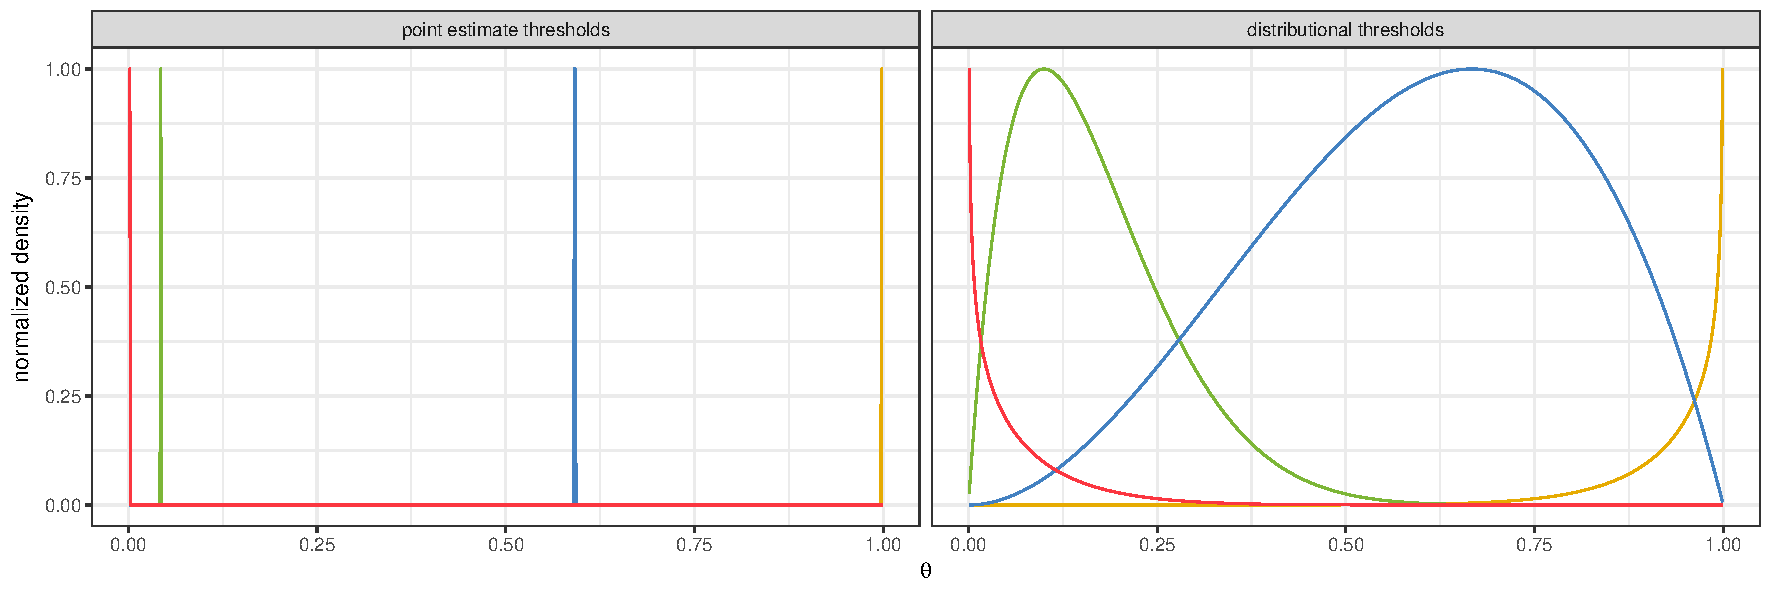
\includegraphics[width=\textwidth]{plots/model-visualization-distributions.pdf}

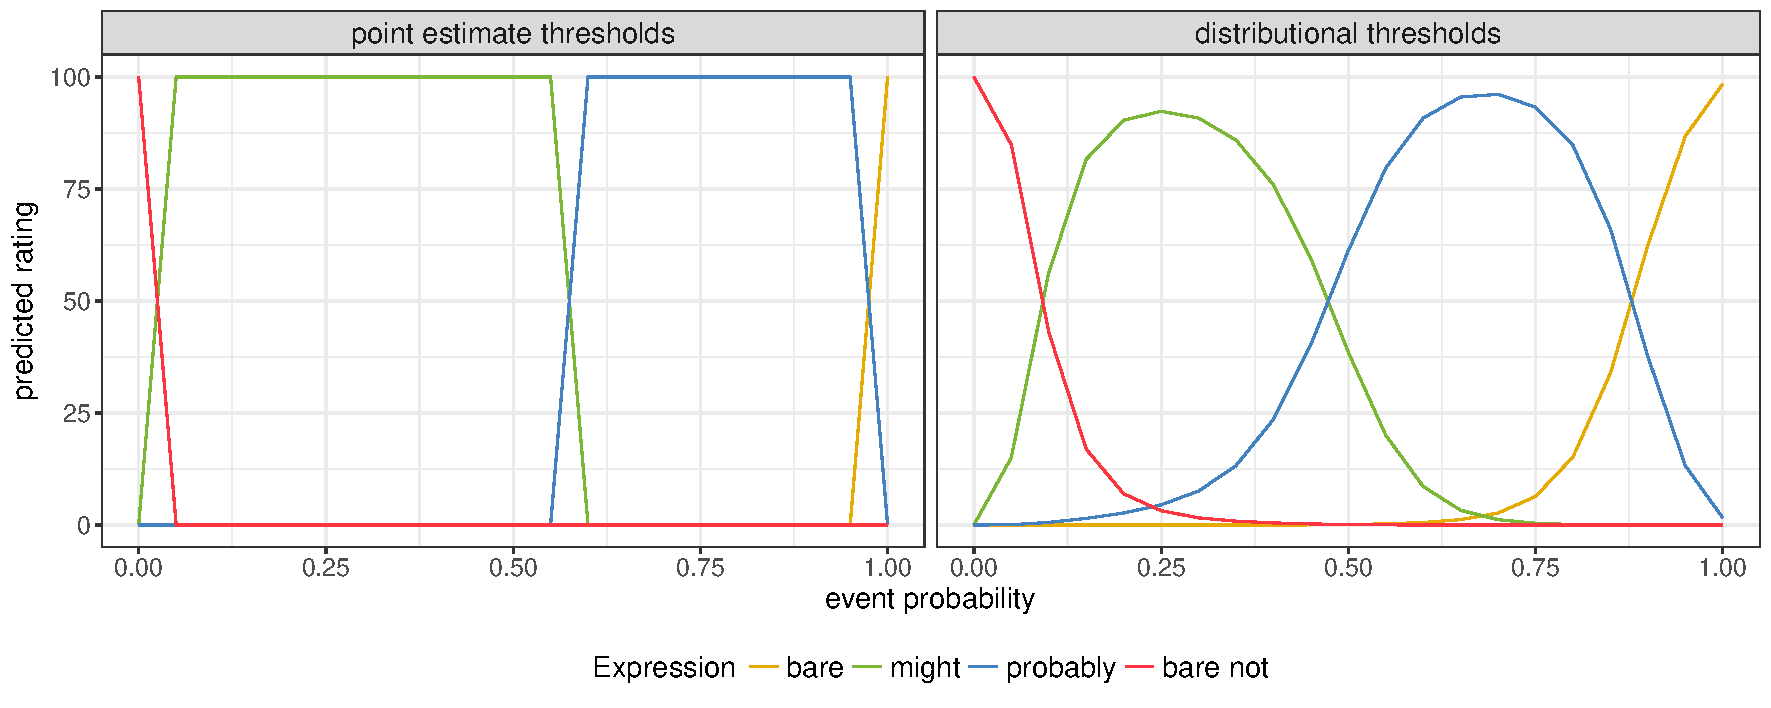
\includegraphics[width=\textwidth]{plots/model-visualization-predictions.pdf}

\caption{Example threshold distributions (upper panels) and corresponding model predictions by the \textit{expected pragmatic speaker} model (lower panels). In this example, the set of possible utterances is $U=\{$\textsc{bare}, \textsc{might}, \textsc{probably}, \textsc{bare not}$\}$, all utterances have equal costs, the rationality parameter $\lambda$ is set to 10, and the prior probability over event probabilities $P(\phi)$ is a uniform distribution. As the panels on the left show, point estimates of thresholds lead to sharp categorical boundaries in the model predictions, whereas distributions over thresholds, as in the panels on the right, lead to gradually increasing and decreasing predicted utterance ratings. \label{fig:model-visualization}}
\end{figure}



$S_1$ crucially depends on a vector of thresholds $\theta$ which contains a threshold for each utterance in $U$, 
as well as  a cost function $c(u)$. The values that speakers and listeners \jd{why speakers AND listeners?} assign 
to these variables are unknown a priori; we infer these values from the data collected in the previously above reported experiment. In our norming studies, we found that both at the population-level and at the individual-level, 
participants' ratings of the different expressions gradually increased and decreased with changing event probabilities 
(as, for example, shown in Figure~\ref{fig:norming-results-indiv}). This is expected if we assume that participants
have probabilistic beliefs about thresholds $\theta$ (as illustrated in the right panels of Figure~\ref{fig:model-visualization}) but not so if we assume that
participants are reasoning based on point estimates of $\theta$ (as illustrated in the left panels of Figure~\ref{fig:model-visualization}).
Considering these observations,  we assume that listeners hold beliefs about speakers' thresholds  in the form of a distribution $P\left(\theta_u\right)$.\footnote{We leave it open 
whether a speaker samples from a distribution over thresholds when making utterances (as suggested by \citet{Qing2015}) 
or always uses the same values for thresholds. In the former case, listeners could have higher-order beliefs  $P(\eta)$ 
about different speakers' threshold distributions instead of having direct beliefs about the thresholds that different 
speakers use. For our purposes, this distinction does not matter since we would assume that listeners marginalize over their higher-order beliefs $P(\eta)$ such that  $P\left(\theta_u\right) = \int P\left(\eta\right) P\left(\theta_u \mid \eta\right) d\eta$ and we therefore take the simplest approach and directly model $P\left(\theta_u\right)$. } Analogously, we assume that listeners also have beliefs $P(c)$ about the speaker's cost function.
Using these two distributions, we can define the \textit{expected pragmatic speaker} $ES_1\left(u \mid \phi \right)$ as follows:

$$ES_1\left(u \mid \phi \right) = \int P(c) \int_0^1 P(\theta) S_1\left(u \mid \phi, \theta, c\right) d\theta \  d c$$

This model predicts which utterance a listener who has uncertainty about a speaker's thresholds (or threshold distributions) \jd{needs to be unpacked, can't be casually thrown into parens :)} and cost function would expect that speaker to use to describe different event probabilities.
Intuitively, this model is a weighted average of different speaker models with differing thresholds and cost functions where the weights are determined by the listener's belief distributions over thresholds
and costs. 

%$P(\theta)$ serves two purposes here: On the one hand, it captures the variability in expectations across participants and on the other hand, it captures individual participants' uncertainty. 
%In theory one could separate these two distributions by having one distribution modeling the variability across participants and then having a separate distribution for each listener capturing
%their uncertainty. Since we are primarily concerned with modeling population-level expectations in this work, we decided to conflate these two source of variability.


%\textbf{TODO:} walk through example model and show how this model is capable of pragmatic inferences and different preferences

\subsection{Linking function}

We assume that in Exp.~1 participants, when asked to provide ratings for utterances, reasoned about what a speaker would say in different situations. 
We assume that these beliefs are guided by participants' beliefs about the speaker's thresholds and costs, and 
that participants are averaging over their uncertainty. For this reason, we assume that the population-level 
average ratings of what participants expect the speaker to say in different situations 
correspond to the probabilities predicted by the \textit{expected pragmatic speaker} model.
However, given the forced choice nature of the experiment and that we are estimating model 
parameters from limited and potentially noisy data, we make the following additional linking assumptions. \jd{this last sentenec ,especially the "However", is weird. what makes the following linking assumptions different from the first? why not say at the beginning that you make n linking assumptions, and then spell out each?}

\begin{itemize}
\item \textbf{Set of utterances}: Across all conditions, we assume that the set of utterances that participants are considering is the set of all utterances that we used in the norming study, i.e., $U= \{$ \textsc{bare}, \textsc{might}, \textsc{probably}, \textsc{think}, \textsc{looks like}, \textsc{could}, \textsc{bare not}$\}$. We include all utterances instead of only the utterances that are presented in a given condition since we assume that participants' general knowledge of English uncertainty expressions also influences their ratings. Ideally, we would include even more utterances in this set of alternatives but since we can only estimate parameters for uncertainty expressions for which we collected ratings, we are limited to the expressions in $U$.

\item \textbf{\textit{something else} option}: Participants in condition $\mathscr{C} = \{u_a, u_b\}$ 
could only choose between the three utterances $U' = \{u_a, u_b,$ \textit{something else}$\}$.
For modeling data from condition $\mathscr{C}$, we therefore need a function to predict the ratings 
for the utterances in $U'$. For $u_a$ and $u_b$, this is straightforward: We assume the probability 
of a participant choosing $u_a$ or $u_b$
is proportional to $ES_1(u_a \mid \phi)$ and $ES_1(u_b \mid \phi)$, respectively. 
We model the probability of a participant choosing the \textit{something else} option as the sum 
of the probability of all utterances that were not part of the condition as well as a constant $O$, 
which accounts for probability mass assigned to utterances that participants might be 
considering but which are not contained in $U$. This gives us the following condition-specific 
function $ES_1^{(\mathscr{C})}$ for predicting participants' ratings.

$$
ES_1^{(\mathscr{C})}(u \mid \phi) \propto 
     \begin{cases}
       ES_1(u \mid \phi) &\quad\text{if } u  \in \mathscr{C}\\
       O + \sum_{u \not \in \mathscr{C}} ES_1(u \mid \phi) &\quad \mbox{if $u$ is \textit{something else}} \\
     \end{cases}
$$

\item \textbf{Cost function}: We assume that the cost function represents participants' beliefs about the speaker's 
preferences for different utterances. Lower costs of an utterance indicate higher speaker preferences. We further 
assume that we are cueing participants to believe that the speaker would be likely to use the two utterances, $u_a$ 
and $u_b$, that are provided in condition $\mathscr{C}=\{u_a, u_b\}$ and that participants therefore primarily use the 
\textit{something else} option when both of the two utterances are semantically infelicitous or otherwise highly unexpected. 
We model this cueing effect in our choice of the cost function $c(u)$, which depends on the condition. For the two utterances 
that are presented to the participants, we set the cost to $1$ and for all the other utterances, we set the cost to a constant $\gamma$:
$$
c(u, \mathscr{C}) = 
     \begin{cases}
       1 &\quad\text{if } u  \in \mathscr{C}\\
       \gamma &\quad\text{otherwise} \\
     \end{cases}
$$

Theoretically, we could have also used a different constant $\gamma_u$ for each utterance. The data from
the norming experiments, However, suggests that participants generally did not prefer one utterance over 
the other. To limit the number of free model parameters and to prevent overfitting, we therefore use a single
constant $\gamma$ for all utterances. We will, However, relax this assumption in our adaptation model in \sectionref{sec:model-adapt}, which
we use to investigate whether listeners are updating their beliefs about preferences during adaptation.

\item \textbf{Noise}: Finally, to account for participants not paying attention or making mistakes, 
we also include a noise term that models participants providing random ratings.
The amount of noise is captured by the noise strength parameter $\delta$. This parameter
indicates the proportion of random responses, that is, the proportion of responses drawn from a uniform distribution
over the three condition-specific responses $U'$. 

\end{itemize}

\noindent Incorporating all of these assumptions, we end up with the following noisy, condition-specific expected pragmatic speaker 
model $ES_1^{(\mathscr{C})'}(u \mid \phi)$, which we use to predict participants' ratings:

$$ES_1^{(\mathscr{C})'}(u \mid \phi) = \delta \times \frac{1}{|U'|} +  (1 - \delta) \times ES_1^{(\mathscr{C})}(u \mid \phi)$$

For the prior distribution over event probabilities $P(\phi)$, which is used in the literal listener $L_0$, 
we use a uniform distribution over the interval $[0,1]$.\footnote{To 
verify the assumption that the prior on event probabilities is uniform, we conducted a separate norming study in which participants rated 
how likely they thought it was that a speaker described different gumball machines containing different 
proportions of blue and orange gumballs after hearing an unintelligible utterance. We found that on average 
participants rated all gumball machines equally likely which suggests that the prior over event probabilities is 
indeed uniform.} For the distributions over thresholds $P(\theta_u)$, we use a Beta distribution parametrized by 
$\alpha_u$ and $\beta_u$. The choice of Beta distributions is motivated by two of its properties. First, the support of a Beta distribution 
is the interval $[0,1]$ which corresponds to the exact range of possible values for $\theta_u$.

Second, depending on the parameterization, Beta distributions can have very different shapes, which is important for 
our assumption that all expressions in the model have a threshold semantics. 
Such a semantics is commonly assumed for uncertainty expressions such as \textit{probably} \citep[e.g.,][]{Yalcin2010,Lassiter2016}, 
but it is unconventional for bare assertions such as \textit{``You'll get a blue one''}. However, since Beta distributions can have a shape 
like the distribution for \textsc{bare} in the upper right panel in Figure~\ref{fig:model-visualization}, the model has the capability to infer
a semantics for the bare form that is almost equivalent to a traditional semantics of bare assertions. In this parameterization of the
Beta distribution, most probability mass is assigned to values of $\theta$ close to 1, which is mathematically almost equivalent to
a traditional semantics.\footnote{Alternatively, one can also see the threshold distribution for the bare form as a distribution over a verification parameter $\eta$ that governs 
how certain a speaker has to be to utter a bare assertion \cite{TODO ask Dan}. Mathematically, our assumption of bare forms having a threshold
semantics is equivalent to assuming that there is a verification threshold $\eta$. \todo{Should we provide a proof in the SI?}}
Therefore, by using Beta distributions for the threshold distributions, we argue that we can treat all expressions in the model the same. \jd{for the naive reader, it will be hard to evaluate how reasonable or unreasonable these different assumptions are. can you include a sentence either at the beginning or the end of this subsection saying which assumptions (and its alternatives) the model is robust to? or flag the assumptions you think are more problematic than others?}


\subsection{Parameter estimation}

Given all the assumptions outlined above, our model has in total $18$ parameters: A cost parameter $\gamma$, a rationality parameter $\lambda$, a noise strength parameter $\gamma$, a constant corresponding to other utterances $O$, and for each utterance, Beta distribution parameters $\alpha_u$ and $\beta_u$. We estimated these parameters jointly from all 21 conditions of the norming study using Bayesian data analysis (see e.g., \cite{Kruschke2014}). To construct the dataset, we treated the ratings by each participant as a probability distribution from which we sampled 10 utterances. We used highly uninformative
uniform priors over the interval $[0,15]$ for all parameters. We estimated the vector of parameters $\Theta$ using MCMC with a Metropolis Hastings sampler. To decrease autocorrelation of the chain, we collected a sample only at every 10th iteration (i.e., we use thinning of 10). We discarded the first 10,000 burn-in samples and then collected 50,000 samples.  We ran four MCMC chains and confirmed convergence by computing the $\hat{R}$-statistic \citep{Gelman1992}. More details on the implementation of the model can be found in the Supplementary Material.

\subsection{Model evaluation}



\begin{figure}
\includegraphics[width=\textwidth]{plots/pre\string_test\string_model\string_main.pdf}
\caption{Model predictions and results from norming study. Error bars correspond to 95\% high density intervals (model predictions) and bootstrapped 95\%-confidence intervals (observed results). \label{fig:norming-results-model-main}}

\end{figure}


The result of the parameter estimation procedure is a posterior distribution over parameters given the observed data $P(\Theta \mid D_{obs})$. We evaluated
the model fit by performing a posterior predictive check (PPC; \cite{Kruschke2014}). To this end, we took 10,000 samples of parameters $\Theta$ from the posterior distribution
and for each sample, we computed the model predictions $ES_{1}^'(u \mid \phi; condition)$ parameterized by $\Theta$. We then compared the average model predictions to the
mean ratings that participants had provided in the pre-exposure experiments. We further computed the 95\% high density interval (HDI; \cite{Kruschke2014}) which reflects the certainty of the model
about its predictions.

Figure~\ref{fig:norming-results-model-main} shows the model predictions and the experimental data for three conditions 
(see Table~\ref{tbl:correlations} and the Supplementary Material for modeling results for all 21 conditions). As these plots show, the model
is able to capture almost the entire variance in participants' average ratings. Further, the 95\% HDIs are very small which suggests
that the model is certain about its predictions. Both of these observations are also true for the model's predictions for all the other
conditions. For 19 of the 21 conditions, the $R^2$ value between the model predictions and the experimental data exceeds 0.9,
and for the remaining 2 conditions, the $R^2$ value exceeds 0.88. 

Most cases in which the model predictions and the experimental data deviate concern the ratings at the two extremes of the event probabilities space.
The model often underpredicts ratings for the \textit{something else} option when there is either a 0\% or a 100\% chance of 
getting a target color gumball. In these situations, participants presumably thought that {\sc bare} and {\sc bare not} are the most appropriate
utterances and therefore rate \textit{something else} highly unless we provide them with the {\sc bare} or {\sc bare not} options. The model predicts
this behavior to some extent but seems to assume that participants were cued more heavily towards the presented utterance options than they actually were.
This could be an indicator that we should revisit our unconventional approach of treating the bare forms like uncertainty expressions with a threshold semantics,
since the model would predict higher ratings for the \textit{something else} at both ends of the scale if we assumed that the bare form and its negation were only true
in the cases of 100\% and 0\% event probabilities, respectively. 
However, for our purposes in this paper, the exact predictions about production choices for objectively certain events are not as important and hence
we decided against revising the assumption that all utterances in the model have a threshold semantics.


One potential concern given the flexibility of the model is that it could be overfitting the data. 
This is unlikely considering that we are estimating only 18 parameters to predict in total 567 data points 
(27 data points for each one of the 21 conditions) but to nevertheless rule out this possibility, we performed a leave-one-out cross-validation of
our model. For each condition $x$, we estimated a distribution over parameters $\Theta_x$ using the data from all conditions but $x$. We then
compared the model predictions of the model parametrized by $\Theta_x$ to participants' ratings in condition $x$. This way, the model has to predict
participant behavior which it has not observed during parameter estimation. Table~\ref{tbl:correlations} shows the $R^2$ values for participants's
ratings and model predictions for the model estimated from all conditions and the leave-one-out models.

\begin{table}
\center
\begin{tabular}{l | c | c}
      Condition & $R^2$ (all data) & $R^2$ (leave-one-out) \\
      \midrule
          bare-might  &  0.992  & 0.988 \\
       bare-probably  &  0.978  & 0.976 \\
          bare-could  &  0.978  & 0.976 \\
     bare-looks like  &  0.927  & 0.896 \\
          bare-think  &  0.968  & 0.964 \\
      might-probably  &  0.964  & 0.954 \\
         might-could  &  0.921  & 0.910 \\
    might-looks like  &  0.934  & 0.918 \\
         might-think  &  0.946  & 0.934 \\
      probably-could  &  0.961  & 0.959 \\
 probably-looks like  &  0.944  & 0.931 \\
      probably-think  &  0.888  & 0.860 \\
    could-looks like  &  0.924  & 0.910 \\
         could-think  &  0.931  & 0.920 \\
    looks like-think  &  0.970  & 0.960 \\
       bare not-bare  &  0.894  & 0.848 \\
      bare not-might  &  0.968  & 0.958 \\
   bare not-probably  &  0.910  & 0.893 \\
      bare not-could  &  0.910  & 0.840 \\
 bare not-looks like  &  0.927  & 0.903 \\
      bare not-think  &  0.933  & 0.920 \\
\end{tabular}
\caption{$R2$ values for experimental data and model predictions for model estimated from all data and for models estimated from all conditions except the predicted condition. \label{tbl:correlations}}
\end{table}


As this table shows, the $R^2$ values remain high even if we exclude the data on which the model is evaluated from the model's training data, 
which suggests that our proposed model indeed explains
participants' expectations of a generic speaker's uncertainty expressions.


\begin{figure}
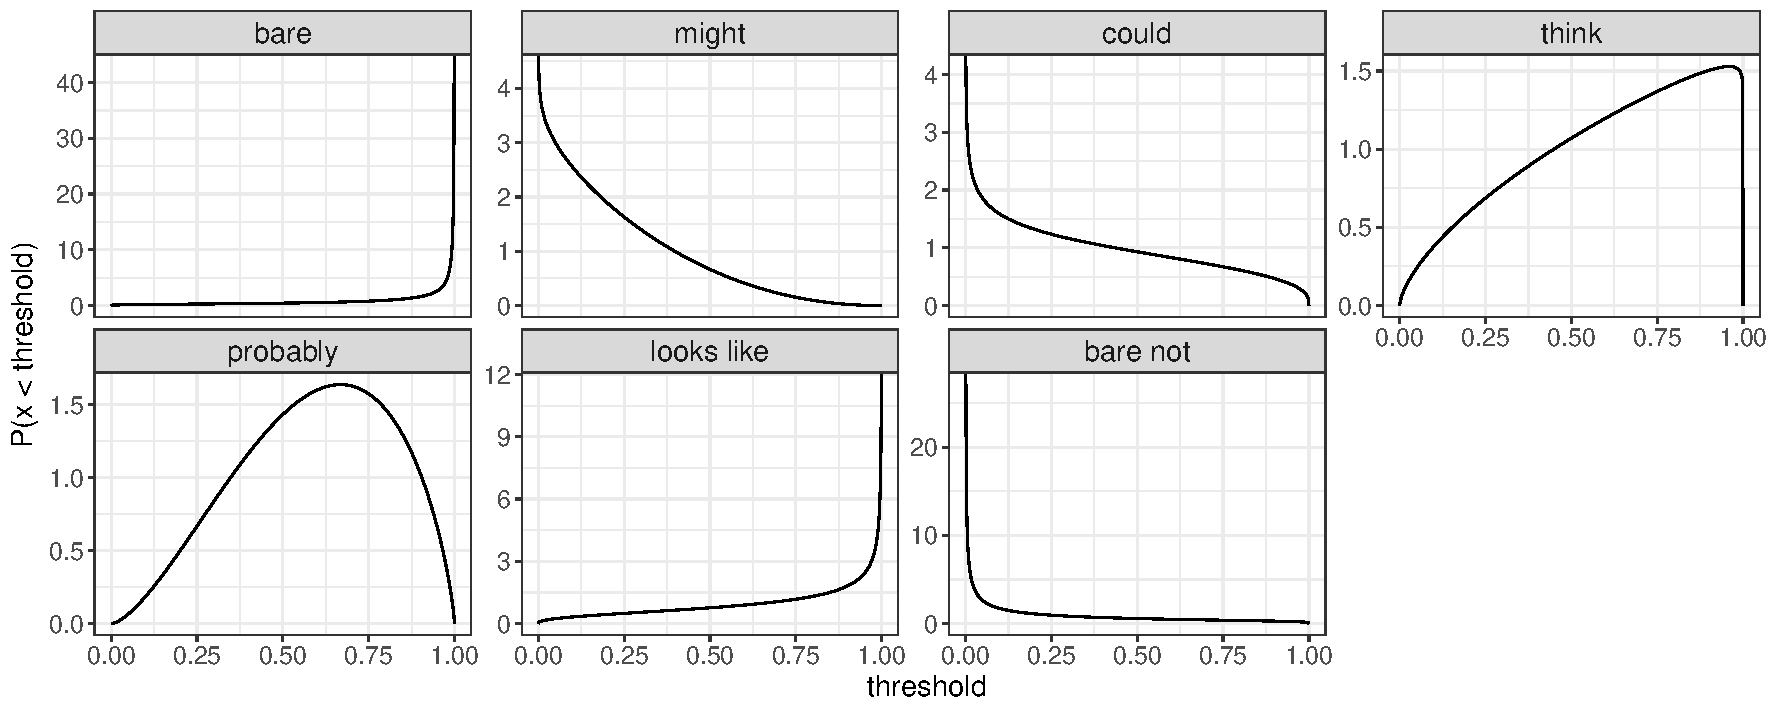
\includegraphics[width=\textwidth]{plots/threshold-distributions-prior.pdf}
\caption{Inferred threshold distributions. For the negative bare utterance (\textsc{bare not}) the distribution corresponds to an upper threshold, i.e., a bare statement embedded under negation is true if the probability of the event is lower than the threshold. For all other utterances, the distributions correspond to a lower threshold.
\label{fig:threshold-distributions}}
\end{figure}

Lastly, one of the advantages of Bayesian cognitive models is that their parameters are interpretable. Figure~\ref{fig:threshold-distributions} shows the 
maximum likelihood estimates of the inferred threshold distributions $P(\theta)$ for the seven uncertainty expressions that we included in our experiments.
As we discussed above, for the bare form and its negation, we expected the model to infer threshold distributions whose probability mass is concentrated 
around $\theta=1$ and $\theta=0$, respectively.\footnote{Note that since the negation of the bare form is a negative form, $\theta$ is an upper threshold. For the bare form as well as
all the other utterances that we are are considering in this paper, $\theta$ is a lower threshold.} As  Figure~\ref{fig:threshold-distributions} shows, this is indeed what
the inferred threshold distributions look like. \jd{would be helpful to say here what the result should have been under a categorical semantic view -- ie distributions peaked on a particular value. highlight that this is NOT what is observed}

The threshold distribution for \textit{might} has most of its probability mass concentrated at values slightly above 0. This 
is in line with non-probabilistic accounts of the interpretation of epistemic modals. These accounts generally assume that \textit{might} $p$ is true 
if there exists \textit{some} world $w$ in a set of (contextually restricted) epistemically accessible worlds $E$ such that $p$ is true in $w$ 
\citep[e.g.,][]{Kratzer1991,Swanson2008,Hacquard2012}. One way to translate this logical condition into our probabilisitic framework is to assume that 
in our gumball machine context, there exists an epistemically accessible world $w$ for each gumball $g$ and that in world $w$, one gets gumball $g$. 
Under this assumption, \textit{``You might get a blue gumball''} is true if there exists an epistemically accessible world $w$  in which one gets a
gumball $g$ that is blue. At the same time, if such a world exists, then $P(\mbox{blue gumball})$ is greater than 0, which approximately corresponds
to the threshold semantics with the inferred threshold distribution of our model. The inferred threshold distribution for \textit{could} is similar to the one of \textit{might}, 
which is again in line with non-probabilistic accounts, which assume that epistemic \textit{might} and epistemic \textit{could} are semantically equivalent \citep{Kratzer1991,Hacquard2012}.

The threshold distribution for \textit{probably} has most of its probability mass concentrated at thresholds above .5. This is again compatible with existing accounts that assume 
that \textit{probably} $p$ is true if $p$ is more likely than the negation of $p$ \citep[e.g.,][]{Kratzer1991}. However, it is also noteworthy, that the inferred
distribution has some probability mass below .5, which empirically corroborates theoretical arguments by \citet{Yalcin2010} that \textit{probably} $p$ can
sometimes also be true if $p$ is less likely than the negation of $p$.

The threshold distributions for the remaining expressions, \textit{looks like} and \textit{think} also match intuitions. The distribution for 
\textit{looks like} has most of its probability mass near threshold values of 1 but is overall slightly weaker, i.e., assigns higher probabilities to lower thresholds,
than the bare form. The distribution for \textit{think} assigns most probability mass to high thresholds, which is compatible with the intuition
that speakers use \textit{think} when they strongly belief in the embedded proposition but are not entirely certain that the proposition is true.
 
 \todo{Include and discuss MAP estimates of other paramerters.}
 
 \subsection{Interim summary}
 
 In this section, we described a computational model of production expectations of uncertainty expressions. This model
 is couched within the RSA framework and assumes that listeners hold beliefs about speaker thresholds (in the form
 of threshold distributions) and about speaker preferences (in the form of cost functions). We estimated 
 the free parameters of this model from the norming data, which resulted in a model that is able to accurately predict
 participant's utterance ratings -- i.e., their expectations of use --  in our norming study across all conditions with a shared set of parameters.
 
 In the following sections of this paper, we will use this model as the basis for modeling adaptation. Since this model
 is able to capture different beliefs about thresholds and preferences, it provides us with the opportunity to simulate 
 the adaptation process as a result of updating beliefs about these model parameters. Further, in order to answer
 our primary research question of whether listeners update their beliefs about lexica or preferences, we can compare
 different adaptation simulations in which we allow different types of parameters to be updated.





\section{Experiment 1: Adaptation of speaker expectations}
\label{sec:exp-prod-adaptation}



We now turn to our main research questions of whether and how listeners adapt to variable uses of uncertainty expressions.
In our norming studies, we found that participants show uncertainty in their expectations about a generic speaker's 
use of \textit{might} and \textit{probably}. Based on these results, we investigate in two experiments whether participants
form speaker-specific expectations about the use of \textit{might} and \textit{probably}.

\subsection{Experiment 1a}
In this experiment, we test whether participants update their production expectations after observing a specfici speaker's use of 
uncertainty expressions for a short period of time. The procedure, materials and analyses were pre-registered at \url{https://osf.io/w926x/}.


\subsubsection{Participants}
We recruited a total of 80 participants (40 per condition) on Amazon Mechanical Turk. 
We required participants to have a US-based IP address and a minimal approval rating 
of 95\%. Participants were paid \$2 which amounted to an hourly wage of approximately 
\$12--\$15. None of the participants had previously participated in the norming study.

\subsubsection{Materials and procedure}

\paragraph{Exposure trials:} In the first part of the experiment, participants saw 20 exposure trials. 
These trials had a similar setup as the trials in the norming study: 
they also showed a child requesting a blue or orange gumball and a gumball machine with blue and orange gumballs. 
However, instead of the cartoon adult, they showed a video of an adult male or female speaker (counterbalanced across participants) producing one of the following six utterances:

\begin{itemize}
\item You'll get a blue/orange one (\textsc{bare})
\item You might get a blue/orange one (\textsc{might})
\item You'll probably get a blue/orange one (\textsc{probably})
\end{itemize}

\begin{table}
\centering
\begin{tabular}{l c c c c c c}
\toprule
& \multicolumn{2}{c}{\sc might} & \multicolumn{2}{c}{\sc probably} & \multicolumn{2}{c}{\sc bare}\\
& $n$ & $\phi$ & $n$ & $\phi$ & $n$ & $\phi$\\
\midrule
\emph{cautious} & {\bf 10} & {\bf 60\%} & 5 & 90\% & 5 & 100\%\\
\emph{confident} & 5 & 25\% & {\bf 10}  & {\bf 60\%} & 5  & 100\%\\  
\bottomrule
\end{tabular}
\caption{Number of exposure trials ($n$) per utterance ({\sc might}, {\sc probably}, {\sc bare}) 
and associated proportion of target color gumballs ($\phi$) in the \emph{cautious} vs.~\emph{confident} 
speaker conditions. Critical trials bolded. \label{tbl:materials}}

\end{table}

The number of trials with each of these utterances as well as the gumball proportions varied across two conditions (see Table \ref{tbl:materials} for an overview). In the {\it confident speaker} condition, participants saw 10 critical trials with 60\% target color gumballs and the speaker producing an utterance with \emph{probably} (target color was randomized across trials), 5 filler trials with 100\% target color gumballs and the speaker producing {\sc bare}, and 5 filler trials with 25\% target color gumballs and the speaker producing {\sc might} condition of the norming study; see \figref{fig:norming-results-main}). In the {\it cautious speaker} condition, participants saw 10 critical trials with 60\% target color gumballs and the speaker producing an utterance with \emph{might}, 5 filler trials with 100\% target color gumballs and the speaker producing {\sc bare}, and 5 filler trials with 90\% target color gumballs and the speaker producing {\sc probably}. The filler trials contained utterance-event probability pairs that were rated very highly in the \textit{might-probably} condition of the norming study (see \figref{fig:norming-results-main}) and were intended to boost confidence in the speaker.

Participants were instructed to watch what the speaker had to say to the child. The video started automatically after a 400ms delay and participants had the option to replay the video as often as they wanted. To advance to the next scene, participants had to press a button which was disabled until the video clip had finished.

\paragraph{Test trials:} The test phase was almost identical to the  \textit{might-probably} condition of the norming study except that the cartoon figure of the man was replaced with a picture of the speaker that participants saw on the exposure trials. Participants were presented with scenes containing gumball machines with 9 different proportions of blue and orange gumballs  (identical as in the norming study) and they were asked to provide ratings for the utterances {\sc might} and {\sc probably} by distributing 100 points across these two utterances and the blanket {\it something else} option. Participants provided two ratings for each of the 18 color-gumball machine combinations resulting in a total of 36 trials. 

Both speakers were from the East Coast and Native Speakers of North American English.\footnote{The first author compensated each of the speakers for their help with the recordings with two slices of marble Guglhupf.} They were instructed to produce the utterances in a normal voice without any special prosody.


\paragraph{Attention checks}  In order to verify that participants were paying attention to the video and the scenes, we included 15 attention checks (6 during exposure and 9 during test trials), which were randomly positioned within the two experimental phases. Trials that contained an attention check either displayed or did not display (pseudo-randomized) a small grey X somewhere around the gumball machine. After completing a trial with an attention check, participants were asked whether they had seen a grey X in the previous scenes or not.

\subsubsection{Exclusions} We excluded participants who provided incorrect responses to more than 3 of the attention checks. Based on this criterion, we excluded 11 participants in the \textit{confident speaker} condition and 8 participants in the \textit{cautious speaker} condition. None of the results reported below depend on these exclusions.


\subsubsection{Analysis and predictions}  

Intuitively, we expect a more confident speaker to use lower thresholds for {\it probably} and {\it might} than a more cautious speaker.
Therefore, if participants track these different uses, we expect their ratings to depend on how the speaker used uncertainty expressions during the exposure phase. 
Concretely,  in our forced choice production paradigm, we expect participants in the \textit{confident speaker} condition to rate {\sc probably} highly for a larger range of event probabilities than participants
in the \textit{cautious speaker} condition. 
Following \cite{Yildirim2016}, we quantified this prediction by fitting a spline with four knots for each expression and each participant and computing the area 
under the curve (AUC) for the splines corresponding to each expression and participant. The area under the curve is proportional to how highly and for how large 
of event probabilities participants rate an utterance. If an utterance is rated highly for a larger range of event probabilities, the AUC will also be larger. 
We therefore tested whether listeners updated their expectations according to these intuitions by computing the difference between the AUC of the spline for 
{\sc might} and of the spline for {\sc probably} for each participant. We predicted that the mean AUC difference would be bigger in the 
\emph{cautious speaker} condition than in the \emph{confident speaker} condition.

\subsubsection{Results and discussion}

\begin{figure}
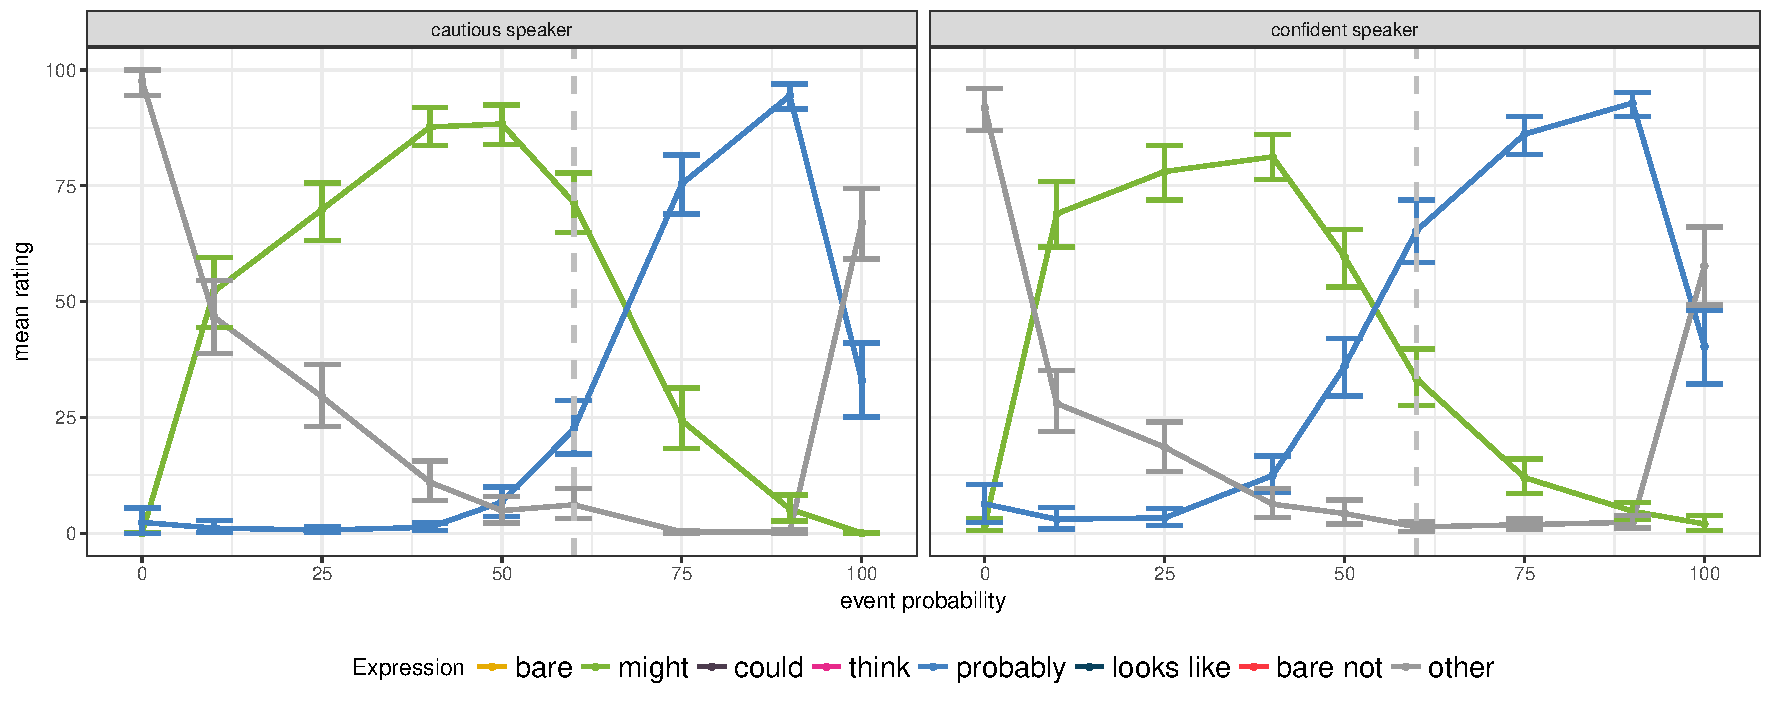
\includegraphics[width=\textwidth]{plots/exp-1-ratings.pdf}
\caption{Mean post-exposure ratings from Experiment 1a. Error bars correspond to bootstrapped 95\%-confidence intervals.  The grey dotted line highlights the ratings for the 60\% event probability ratings.  \label{fig:adaptation-results-prod}}
\end{figure}

\begin{figure}
\center
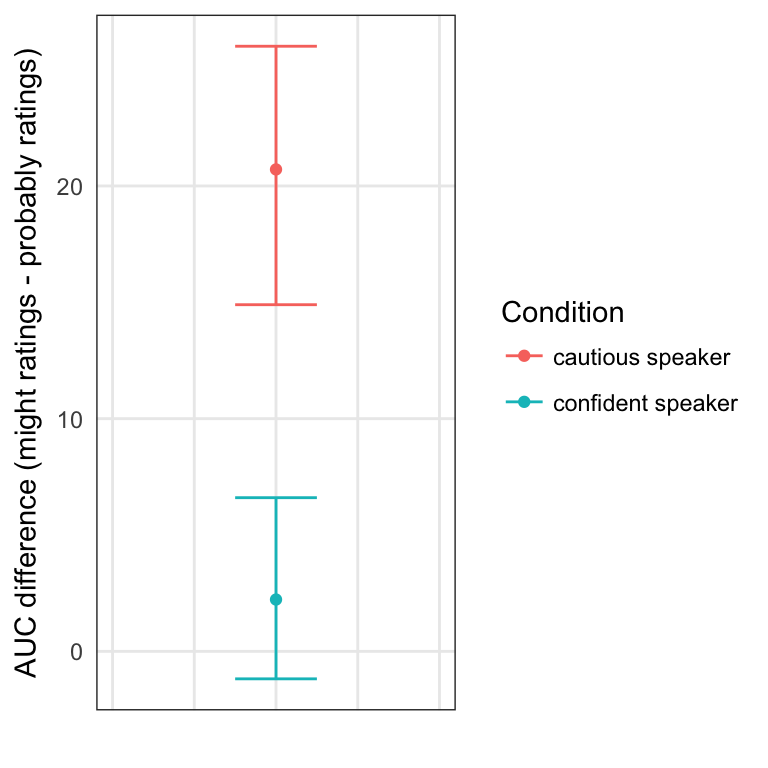
\includegraphics[width=.5\textwidth]{plots/adaptation-auc-production.png}
\caption{Area under the curve (AUC) differences from Experiment 1. Error bars correspond to bootstrapped 95\%-confidence intervals.  \label{fig:adaptation-auc-prod}}
\end{figure}

Figure~\ref{fig:adaptation-results-prod} shows the mean ratings for the three options in the two conditions. As these plots show, participants updated their expectations about the speaker's language use and therefore made different predictions about how the speaker would use uncertainty expressions. In the \emph{cautious speaker} condition, participants gave high ratings for {\sc might} for a larger range of event probabilities than in the \emph{confident speaker} condition. On the other hand, participants gave high ratings for {\sc probably} for a larger range of gumball proportions in the \emph{confident speaker} condition than in the \emph{cautious speaker} condition. These differences result in a significantly bigger AUC difference in the \emph{cautious speaker} condition than in the \emph{confident speaker} condition ($t(59) = 4.98$, $p < 0.001$, see also Figure~\ref{fig:adaptation-auc-prod}).

As Figure~\ref{fig:adaptation-results-prod} shows, participants also differed in their ratings of the two utterances when they were presented with a scene with 60\% target color gumballs. In the {\emph cautious speaker} condition, participants rated {\sc might} higher than {\sc probably}; in the {\emph confident speaker} condition, the pattern was reversed and participants rated {\sc probably} higher than {\sc might}. These expectations mirror the speaker behavior during the exposure phase and provide additional evidence that participants tracked the speaker's usage of uncertainty expressions. 

%Our results also seem to rule out an alternative explanation according to which participants were inferring higher-level speaker goals rather than forming expectations about the speaker's language use. For example, prima facie, it could be that participants inferred that the  \textit{confident speaker} wanted to appear encouraging towards the child. However, if participants inferred such a higher-level goal, then we would expect participants to belief that the speaker would use utterances that are even more encouraging when there is a high probability of getting a target color gumball, resulting in higher ratings of the \textit{something else} option for high event probabilities. We did not observe such an effect, and  in fact, numerically, the rating of \emph{something else} was higher in the \emph{cautious speaker} condition than in the \textit{confident speaker} condition.

Our results further suggest that participants are updating their mappings between uncertainty expressions and event probabilities: In the {\it confident speaker} condition, {\sc might} and {\sc probably} were rated highly for lower event probabilities than in the {\it cautious speaker} condition. However, one potential confound in this experiment is that the number of utterances with \textit{might} and \textit{probably} differed across the two conditions (see Table~\ref{tbl:materials}). It could therefore be, that participants only learned that the {\it cautious speaker} overall prefers to use {\sc might} and the {\it confident speaker} prefers {\sc probably}. We therefore conducted another experiment in which we balanced the number of exposures to {\sc might} and {\sc probably} in both conditions.

\subsection{Experiment 1b}

In this experiment, we aim to replicate the results from Experiment~1a and test whether listeners are updating their 
mappings between the uncertainty expressions and event probabilities when they are exposed to a speaker who
uses \textit{might} and \textit{probably} with the same frequency.  The procedure, materials and analyses were pre-registered at \url{https://osf.io/qnam7}.
\subsubsection{Participants}
We recruited a total of 80 participants (40 per condition) on Amazon Mechanical Turk. 
We required participants to have a US-based IP address and a minimal approval rating 
of 95\%. Participants were paid \$2.20 which amounted to an hourly wage of approximately 
\$12--\$15. None of the participants had previously participated in the norming study.

\subsubsection{Materials and procedure}

Materials, conditions, and procedure were identical as in Experiment~1a except that we added 5 additional fillers such
that the frequency of \textsc{might} and \textsc{probably} was the same (10 utterances per expression) in both conditions.

\subsubsection{Analysis and predictions}  

The analysis was identical as in Eperiment~1a. We again predicted that the mean AUC difference would be bigger in the 
\emph{cautious speaker} condition than in the \emph{confident speaker} condition.

\subsubsection{Exclusions} We used the attention checks and exclusion criteria as in Experiment~1a.  Based on these criteria, we excluded 8 participants in the \textit{cautious speaker} condition, and 7 participants in the \textit{confident speaker} condition.

\subsubsection{Results and discussion}

\begin{figure}
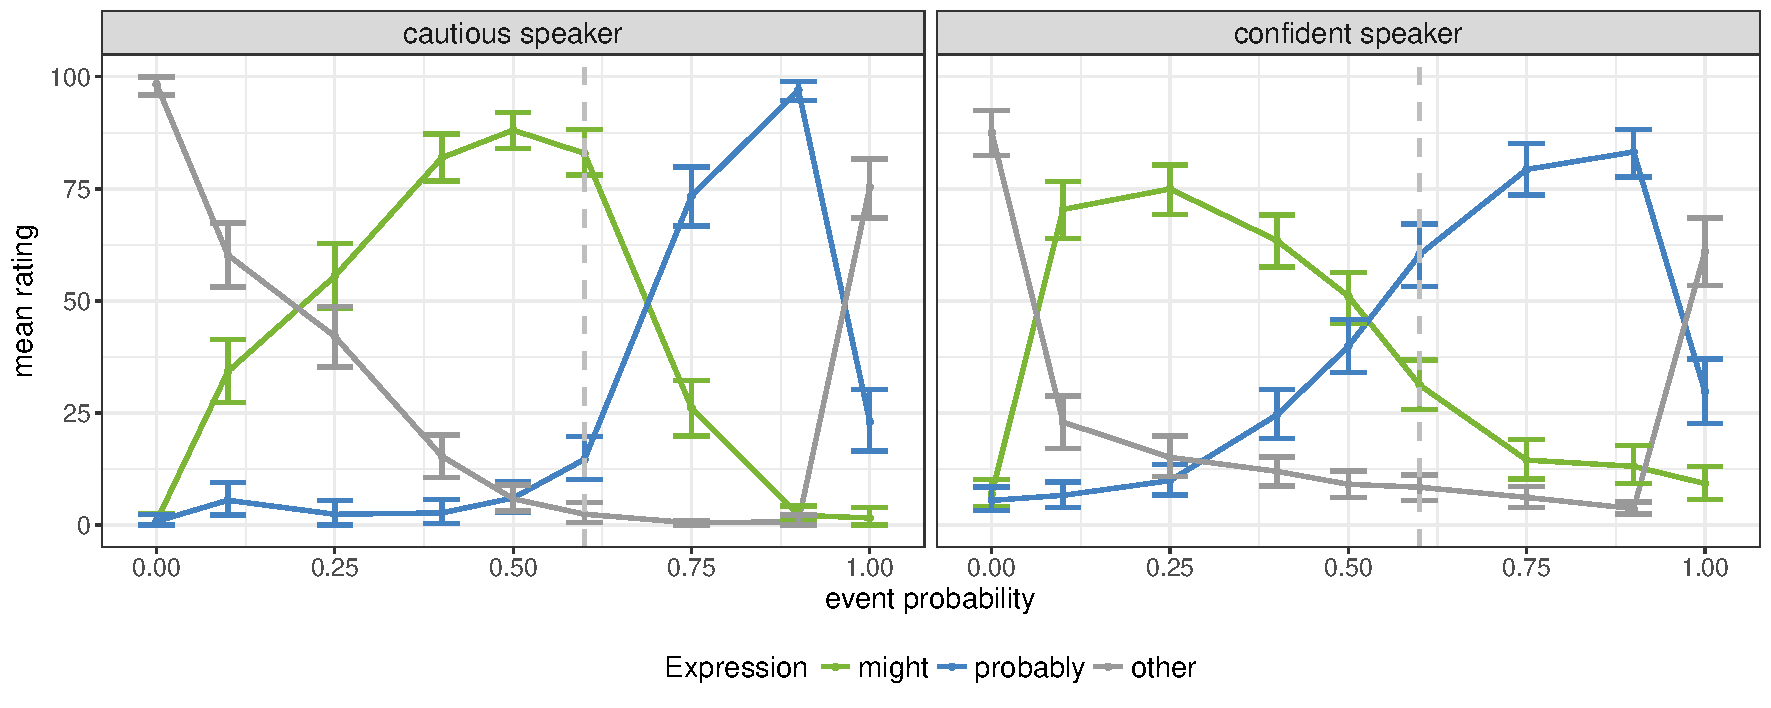
\includegraphics[width=\textwidth]{plots/exp-1-replication-ratings.pdf}
\caption{Mean post-exposure ratings from Experiment 1b. Error bars correspond to bootstrapped 95\%-confidence intervals.  The grey dotted line highlights the ratings for the 60\% event probability ratings.  \label{fig:adaptation-results-prod2}}
\end{figure}

Figure~\ref{fig:adaptation-results-prod2} shows the mean ratings for the three options in the two conditions. As these plots show, participants updated their expectations about the speaker's language use also in this experiment and the
AUC difference was bigger in the \emph{cautious speaker} condition than in the \emph{confident speaker} condition ($t(63) = 2.99$, $p < 0.01$). 

This experiment provides evidence against an account according to which participants only learn that the \emph{cautious speaker} prefers to use {\sc might} and the {\it confident speaker} prefers {\sc probably}. 
Since the frequency of both expressions was the same in this experiment, participants could not have inferred a preference for one of these two utterances and therefore we would not expect different ratings if participants
had only tracked the frequencies of the utterances. 

In summary, the results from our two experiments provide evidence for listener adaptation to a specific speaker's use of uncertainty expressions after a brief exposure phase. Further, taken together, these experiments
suggest that listeners' expectations about a speaker's language use are at least not exclusively driven by tracking speaker's preferences for different utterances. We investigate the nature of speaker-specific expectations
in the next section.


% 

\section{Adaptation model}
\label{sec:model-adapt}



The experimental results presented in the previous section suggest that listeners are updating 
\textit{some} expectations about language use when they are interacting with a speaker. 
However, what kind of expectations listeners are updating is unclear. As we mentioned before, 
there seem to be three likely representations that are being updated: 
it could be that listeners are updating their expectations about the speaker's lexicon 
(i.e., the mapping between event probabilities and uncertainty expressions); 
it could be that listeners are updating their expectations about the speaker's preferences; 
and it could be that listeners are updating their expectations about both the speaker's lexicon 
and the speaker's preferences. The experimental results above suggest that it is unlikely that listeners are tracking only speaker preferences but considering
that beliefs about preferences and beliefs about the lexicon can interact in complex ways (as illustrated in \figref{fig:inference-example}), we are considering all three options.

The production expectation model in \sectionref{sec:model-baseline} provides us with the opportunity to formally evaluate these three hypotheses.
Through a series of simulations of the adaptation process, we can compare models in which different types of parameters are
being updated during adaptation. Following work in modeling adaptation in other linguistic domains \citep[e.g.,][]{Kleinschmidt2012,Kleinschmidt2015}, 
we assume that in interaction, listeners form beliefs about a set of speaker-specific parameters $\Theta_S$. 
We further assume that the formation of these beliefs is an instance of Bayesian belief updating:
listeners start off with prior beliefs about $\Theta_S$ based on their general knowledge about 
language and subsequently update their beliefs about $\Theta_S$ with every utterance they hear. 
That is, after observing a series of productions $D={d_1, ..., d_n}$ where each $d_i$ is an 
utterance-event probability pair $d_i = (u_i, \phi_i)$, listeners beliefs about $\Theta_S$ are the result
of performing Bayesian inference:
$$P(\Theta_S \mid D) \propto P(\Theta_S) P(D \mid \Theta_S) = P(\Theta_S) \prod_{i=1}^nP(d_i \mid \Theta_S) $$

\noindent We assume that the likelihood function is the \textit{expected pragmatic speaker} $ES_1$ parameterized by $\Theta_S$:

$$P(\Theta_S \mid D) \propto P(\Theta_S)  \prod_{i=1}^n ES_1(u_i \mid \phi_i, \Theta_S) $$



\subsection{Simulations}

Our adaptation model crucially relies on a prior over speaker-specific parameters $P(\Theta_S)$
which reflects listeners prior beliefs about the use of uncertainty expressions. For our simulations,
we assume that the means of this prior are given by the estimates of the model parameters that 
we obtained from fitting the model to the norming data.
In order to investigate which kind of parameters are updated during adaptation, we run simulations
with different prior structures, which lead to different parameters being updated during adaptation.

\begin{itemize}
\item \textbf{\textit{Costs}}: The first prior structure corresponds to an adaptation process according to which participants only learn speaker preferences during adaptation. 
We use a log-normal distribution centered at the mean value that we inferred from the norming data for the prior over cost parameters. Since we are interested in whether listeners are updating their beliefs about speaker preferences, we relax the assumption from the norming study that all utterances have the same cost and assume that each expression has its own cost parameter indicating beliefs about the speaker's preferences. We model the prior as a log-normal distribution for two reasons: First, the cost has to be greater than zero and the support of log-normal distributions is limited to numbers greater than 0. Second, since the cost term is part of an exponent in the expected pragmatic speaker model, differences on a logarithmic scale correspond to linear differences in the model's utterance probabilities. For the priors over all other parameters, we use a delta distribution, i.e., a distribution with zero variance, which means that all the other parameters cannot be updated in the model simulations.
\item \textbf{\textit{Threshold distributions}}:  This prior structure corresponds to an adaptation process according to which participants only learn speaker-specific threshold distributions during adaptation. We parameterize the Beta distributions $P(\theta_u)$ with their mean $\mu_u$ and population parameter $\nu_u$ \citep{Kruschke2014}. Since the threshold and therefore also the mean of the threshold distribution have to lie within the interval [0,1], we use a truncated normal distribution $\mathscr{N}_{[0,1]}$, which we center at the mean value from the norming data. For the population parameters $\nu_u$, which indicates how peaked a threshold distribution is, we assume that distributions can only become more peaked when they are exposed to a speaker with very consistent language use and therefore model the prior as an exponential distribution shifted to the mean population parameter that we estimated from the norming data. We use a delta distribution for the priors over all other parameters.
\item  \textbf{\textit{Threshold distributions and costs}}:   This prior structure corresponds to an adaptation process according to which participants learn both speaker-specific threshold distributions and speaker preferences during adaptation.  We use the log-normal distributions as priors over the cost parameters and the truncated normal and exponential distributions as priors over the threshold distribution parameters. This means that both the threshold distributions and the cost parameters can be updated during the adaptation simulations.
\end{itemize}

Each of these prior structures corresponds to a different hypothesis about what kind of expectations listeners are updating during adaptation. For comparison, we also consider a baseline in which none of the parameters are updated during adaptation (the {\it fixed} prior structure). To adjudicate between these three hypotheses, we ran simulations of the adaptation process for both conditions with different prior structures and compared the models in terms of their likelihood of generating the experimental data.
We ran a separate simulation for each of the two experimental conditions (\textit{cautious speaker} and \textit{confident speaker})  but crucially always used the same priors for the two simulations. During each simulation, we performed Bayesian inference to infer the posterior distribution after observing the 20 utterances that participants had seen in the exposure phase (see Table~\ref{tbl:materials} for an overview of the 20 utterances in the two conditions). We performed inference using MCMC with a Metropolis-Hastings sampler. We used thinning of 10, discarded the first 2,000 burn-in samples and collected 10,000 samples from each of the two chains.

The prior distributions over the different parameters that may be updated during the adaptation simulations are all parameterized by two constants which govern their mean and their variance. The first set of parameters (the mean of the log-normal and truncated normal distributions; the location parameter of the exponential distributions) was given by the estimates from fitting the model to the norming data. The second set of parameters (the variance of the log-normal and truncated normal distributions; the scale parameter of the exponential distributions) was treated as hyperparameters of the simulations. To keep the model as simple as possible, we only used three hyperparameters in total: a variance parameter for the cost for all expressions; a variance parameter for the mean of the threshold distributions for all utterances; and a scale parameter for the prior over population parameters for all utterances. We optimized these three parameters through a Bayesian hyperparameter search on the adaptation data, which provided us with a distribution over hyperparameter values. Considering that each simulation is computationally expensive, we could only test a few hundred hyperparameter combinations, which are listed in \todo{Table~XXX}. We found that the resulting distributions were highly peaked and therefore, we used only the maximum a posteriori estimates of the hyperparameters (also shown in \todo{Table~XXX}) for the model comparisons below.


\subsection{Model comparisons}

We compare the models fits according two metrics. First, we consider the $R^2$ value between participants' average post-exposure ratings and the maximum a posteriori predictions of the post-exposure model. Second, we compute the likelihood of the model generating the post-exposure data. For the latter, we constructed a dataset $D_{obs}$ of utterance-event probability pairs by treating each post-exposure rating as a probability distribution and sampling 10 utterances from it. We then computed the posterior likelihood odds between Model 1 with posterior distribution over parameters $P(\Theta_{S}^{(1)})$ and Model 2 with posterior distribution $P(\Theta_{S}^{(2)})$.

$$\mbox{posterior likelihood odds} = \frac{\mathlarger{\int_0^1} {P\left(\Theta_{S}^{(1)}\right) P\left(D_{obs} \mid \Theta_{S}^{(1)} \right) d   \Theta_{S}^{(1)}}}{\mathlarger{\int_0^1} P\left(\Theta_{S}^{(2)}\right) P\left(D_{obs} \mid \Theta_{S}^{(2)}\right)d   \Theta_{S}^{(2)} }$$
 
\noindent The posterior likelihood odds indicate how much more likely it is that the data was generated by Model 1 than by Model 2. Since we are marginalizing over a distribution over parameter values, this comparison of models will naturally
favor simpler models. For a more complex model with more parameters, the distribution over different parameter values will be more disperse and can contain more parameter configurations that lead to a low likelihood of the data.

\begin{table}
\center
\begin{tabular}{r | c | c  }
Model & $R^2$ &   odds  \\ \midrule
fixed & 0.746 & $10^{-1200}$    \\
cost & 0.770 &  $10^{-448}$    \\
threshold distributions & 0.874 &  $10^{-284}$   \\
cost \& threshold distributions & 0.815 & 1 \\
\end{tabular}
\caption{Model evaluation results on data from Experiment~1a. $R$\textsuperscript{$2$} are computed between  the mean post-exposure ratings and the mean model predictions. \textit{odds} are the posterior likelihood odds of the models compared to the \textit{cost and threshold distributions} model. \label{tbl:model-comparison}}
\end{table}

\begin{table}
\center
\begin{tabular}{r | c | c }
Model & $R^2$ &   odds  \\ \midrule
fixed & 0.662 & $10^{-1248}$    \\
cost & 0.802 &  $10^{-458}$  \\
threshold distributions & 0.877 & $10^{-212}$  \\
cost \& threshold distributions & 0.875 & 1 \\
\end{tabular}
\caption{Model evaluation results on data from Experiment~1b.  $R$\textsuperscript{$2$} are computed between  the mean post-exposure ratings and the mean model predictions. \textit{odds} are the posterior likelihood odds of the models compared to the \textit{cost and threshold distributions} model.  \label{tbl:model-comparison-replication}}
\end{table}

Table~\ref{tbl:model-comparison} shows the $R^2$ values between the four models and the experimental data from Experiment 1a 
as well as the posterior likelihood odds. As the values in this table show, the model in which the cost as well as the threshold 
 distributions are updated during adaptation is much more likely to generate the experimental data than the other 
 two less complex models. However, this is not entirely reflected in the $R^2$ values between the mean model predictions
 and the mean model predictions. Similarly to the posterior odds, the $R^2$ values suggest that the \textit{fixed} model
 and the \textit{cost} model make worse predictions than the other two models. At the same time, the two metrics disagree on the 
 ranking of the \textit{threshold distributions} and \textit{cost and threshold distributions} models -- the $R^2$ values suggest
 that the model according to which only the threshold distributions are updated during adaptation predicts 
 participants' post-exposure behavior best.
 
 To assess the stability of these results, we conducted another series of simulations to predict the post-adaptation
 ratings from Experiment~1b. For these simulations, we used identical prior structures and parameterizations as in
 the previous simulations, i.e., we did not optimize any hyperparameters of the model. However, 
 since participants saw additional 5 filler utterances during the exposure phase, we also exposed the model to 5 additional utterances. 
 The model 
evaluation results for these simulations are shown in Table~\ref{tbl:model-comparison-replication}. As the likelihood odds
in this table show, the model in which both the costs and the threshold distributions can be updated is again much more
likely to generate the experimental data than the other two models. This replicates the findings from the previous simulations.
According to the $R^2$ metric, the \textit{threshold distributions} and \textit{cost and threshold distributions} models predict
the data approximately equally well.

What do these modeling results tell us about the semantic/pragmatic adaptation process? 
We assumed that each of these simulations
correspond to an adaptation process in which different types of expectations are being updated.
The modeling results strongly corroborate the experimental results from Experiments~1a and 1b since
the models according to which no expectations are being updated during adaptation (the \textit{fixed} model) 
or according to which only preferences are being updated (the \textit{cost} model) provide poor predictions of the post-adaptation
ratings. The results also clearly indicate that listeners are updating expectations about the threshold distributions. Independent of
the metric, the models according to which listeners are updating threshold distributions were best at predicting post-adaptation
behavior in all simulations. 

However, in terms of the $R^2$ metric, it remains unclear whether adaptation is a result of 
participants updating expectations about threshold distributions or threshold distributions and preferences. 
In part, this inconsistency can most likely be explained by the properties of the $R^2$ metric. For one, unlike the posterior odds, 
it does not take uncertainty of the model predictions into account but rather compares the mean participant behavior to the mean 
model predictions. Considering that the model does exhibit considerable uncertainty in its post-exposure rating predictions, it is not
particularly surprising that the two metrics suggest different conclusions.\footnote{See \citep{Gelman2018} for a proposal of a Bayesian $R^2$ value.}
Second, since the ratings and the model predictions are probability distributions, 
the empirical and predicted ratings for one utterance for a specific event probability are not independent 
of the ratings for other utterances and therefore not all assumptions for using $R^2$ are met. Considering these
factors, one should trust the posterior odds more than the $R^2$ values, which suggests that there is strong evidence that listeners 
are updating expectations about {threshold distributions} as well as {preferences}. We nevertheless, still consider and discuss both possibilities
again in \sectionref{sec:exp-model-interpretation}.



\subsection{Model evaluation}

\begin{figure}
  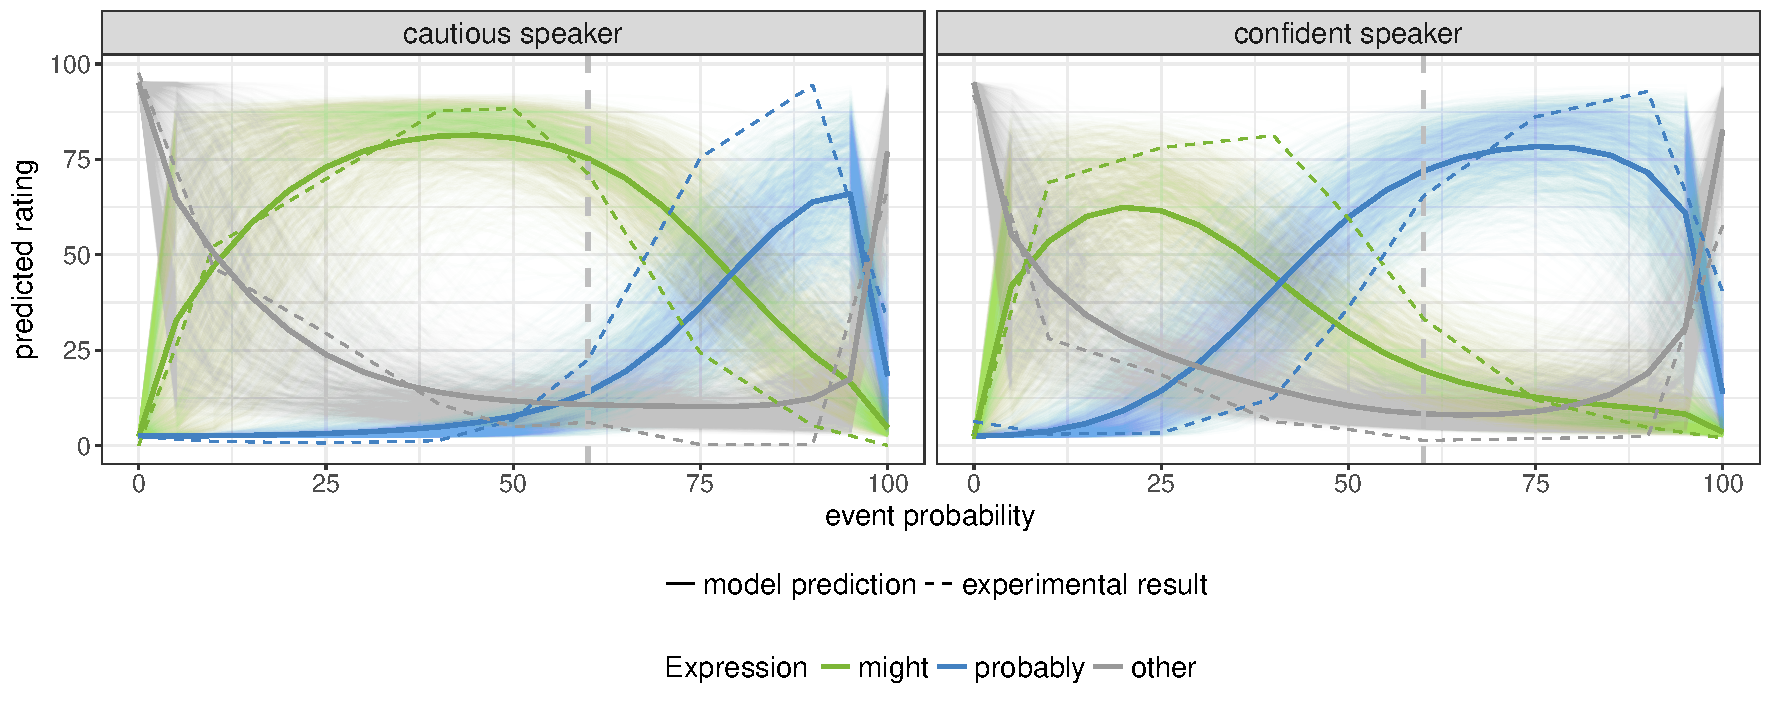
\includegraphics[width=\textwidth]{plots/adaptation-posterior-predictions.pdf}
  \caption{Post-adaptation model predictions and experimental results. 
  The solid lines shows the mean model predictions and the shades around the mean indicate the distribution of model predictions. \label{fig:post-exposure-model}}
\end{figure}

Apart from quantitatively assessing the fit of the model, we can also visually inspect the predictions of the model. 
Figure~\ref{fig:post-exposure-model} shows the post-exposure predictions of the \textit{cost \& threshold distributions} model compared to the average participant ratings for the two conditions. Qualitatively, 
the model captures several important patterns in the post-adaptation behavior. The model correctly predicts that in the \textit{cautious speaker} condition, ratings for \textsc{might} are 
higher than ratings for \textsc{probably} when there is an objective probability of 0.6. For the \textit{confident speaker} condition, the model correctly predicts the
opposite pattern. The model also predicts that in the \textit{cautious speaker} condition, participants rate \textsc{might} highly for a larger range of event probabilities than
in the \textit{confident speaker} condition and the model predicts the  reverse pattern for the \textsc{probably} ratings. Further, the model predicts that high ratings for \textsc{might} 
and \textsc{probably} are not limited to the utterance-event probability combinations that participants observed during the exposure phase. For example, the model correctly predicts
high ratings of \textsc{might} for low event probabilities in the \textit{cautious speaker} condition despite the fact that it never observed utterances for low event probabilities. Similarly,
the model predicts high rating of \textsc{probably} for high event probabilities in the \textit{confident speaker} condition -- a combination which was again not part of the exposure trials
of this condition.

Quantitatively, there are some differences between the model predictions and participant behavior. This is not surprising considering that the model predictions are a result of simulations
and, with the exception of the three variance parameters of the prior distributions, we did not fit the model parameters to the behavioral data. One difference is that the model underpredicts 
the ratings of one of the filler utterances in both conditions: in the \textit{cautious speaker} condition, the model underpredicts ratings of \textsc{probably}; in the \textit{confident speaker} condition, it underpredicts
ratings of \textsc{might}. One reason for this deviation could be the relatively simple prior structure. For the priors, we made the assumption that all model parameters are independent of each other and 
that the variance for the different parameter types is the same for all utterances. However, it could be that listeners have more structured prior beliefs such that priors over different parameters are correlated or
variances of prior distributions differ. For example, it could be that listeners expect the thresholds for \textit{might} and \textit{probably} to be correlated such that higher thresholds for \textit{might} are correlated 
with higher thresholds for \textit{probably}. Or it could be that listeners expect more between-speaker variation for some expressions than for others. Considering that we have only data from two experiments to test
our model predictions and therefore we would likely overfit to our data if we tried to fit more complex prior structures with more parameters, we leave  the investigation of the exact structure of listeners prior beliefs to future work.

\begin{figure}
  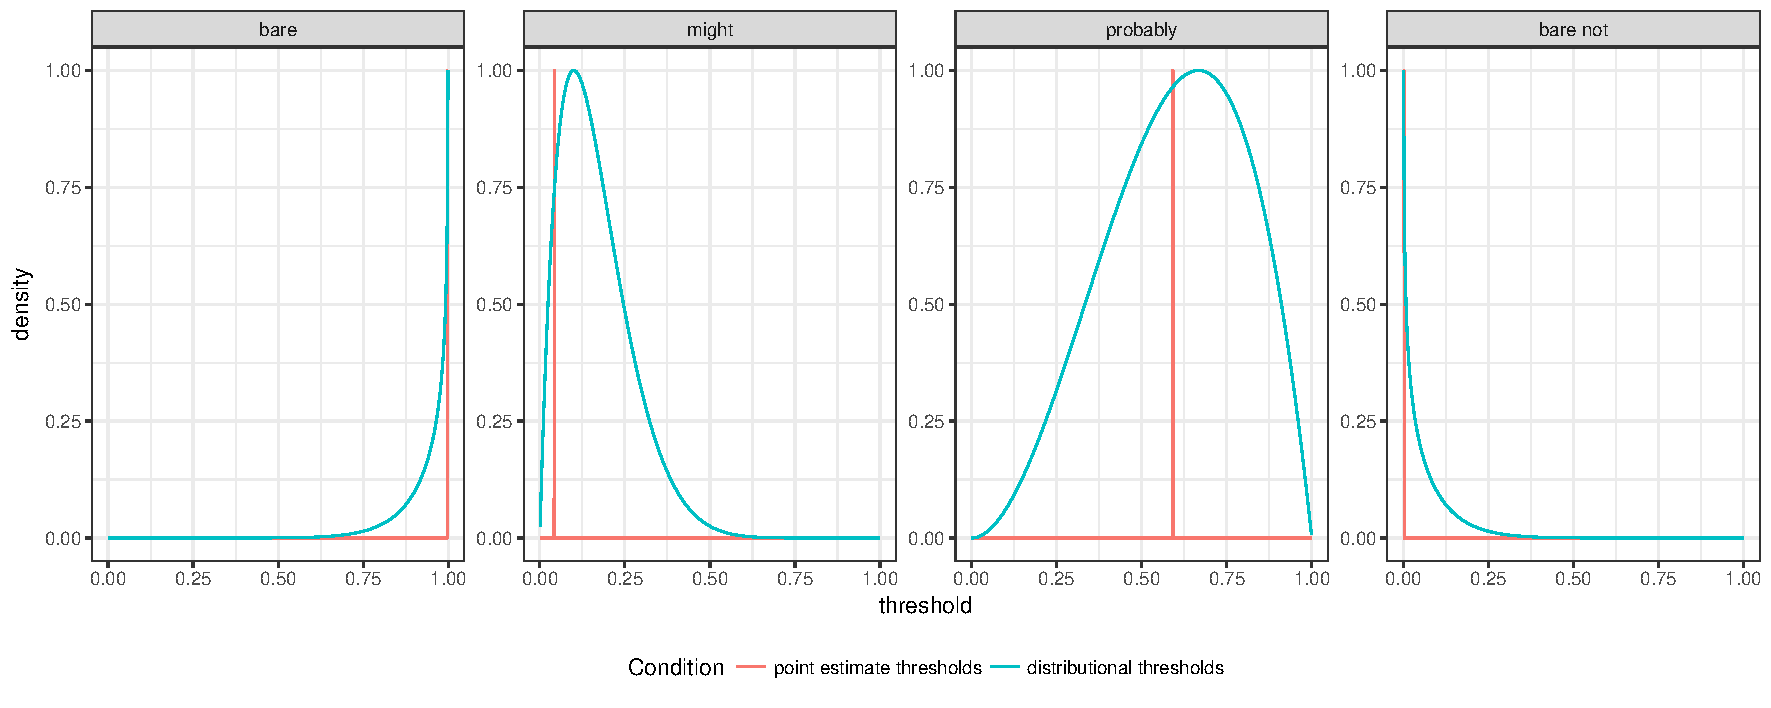
\includegraphics[width=\textwidth]{plots/adaptation-posterior-thresholds.pdf}
  \caption{Post-adaptation threshold distributions. \label{fig:post-exposure-thresholds}}
\end{figure}




The second noticeable deviation is that the model overpredicts the ratings of the \textsc{other} utterance for event probabilities of 1. This prediction is primarily driven by high values for the predicted ratings of \textsc{bare}. In
this case, However, it appears that the model is making correct predictions and that the lower ratings by participants are an artifact of the experimental task. After completing the experiment, 
several participants indicated in a feedback form that they were confused by the lack of an option to rate the \textsc{bare} utterance, 
which they had heard during the exposure phase. In light of this confusion, almost all individual participants chose among two strategies when there was an event probability of 1: they either provided a rating of 100 for \textsc{other} 
or they provided a rating of 100 for \textsc{probably}, which on average leads to the ratings shown in \figref{fig:post-exposure-model}.

Except for these two deviations, the model also makes accurate quantitative predictions of the post-exposure ratings.

Lastly, we can also inspect how the model arrived at its predictions by looking at the inferred model parameters.  
Figures~\ref{fig:post-exposure-thresholds} and \ref{fig:post-exposure-costs} show the inferred
post-exposure threshold distributions and costs for the two conditions as well as the distributions inferred from the norming data.
Figure~\ref{fig:post-exposure-thresholds} shows that the threshold distribution for \textit{probably}
changed considerably depending on the exposure phase: in the \textit{cautious speaker} condition,
its mean shifted to a higher value than we inferred from the norming data; in the \textit{confident speaker} condition the mean 
shifted to a lower value. To a lesser extent, we observe similar shifts in the mean of the threshold
distributions for \textit{might}. We further observe that for all expressions, the variance of the threshold
distributions decreased as a result of adaptation. In the case of the expressions that were part of the exposure
phase, this is expected, since the exposure speaker used these expressions very consistently; in the case of the
other expressions, this decrease in variance is a result of the exponential prior over the population parameter,
which biased the model towards lower variance. For some of the thresholds, this resulted in differently shaped distributions.
However, note that the area under the curve of all threshold distributions except for \textit{probably} is still very similar to the 
area under the curve of the norming data threshold distributions. And overall, except for the distributions
for \textit{might} and \textit{probably}, the post-exposure threshold distributions are almost identical in both conditions.
This suggests that the post-adaptation expectations 
are in part a result of updated threshold distributions for \textit{might} and \textit{probably}.

\begin{figure}
\center
  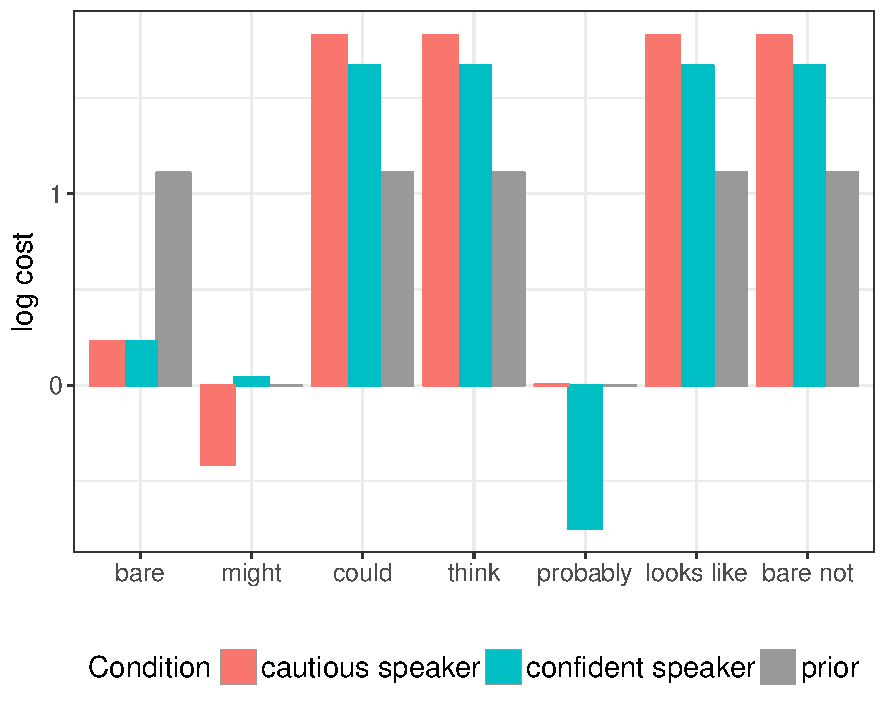
\includegraphics[width=0.5\textwidth]{plots/adaptation-posterior-costs.pdf}
  \caption{Inferred post-adaptation $log$ cost values. Note that the cost of \textsc{might} and \textsc{probably} 
  in the norming data model was 1 and therefore the $log$ cost for these utterances is 0.  \label{fig:post-exposure-costs}}
\end{figure}

Figure~\ref{fig:post-exposure-costs} shows that the costs of the \textsc{might}, \textsc{probably} and
\textsc{bare} utterances, i.e., the three utterances that participants observed during the exposure phase,
all decreased while the costs of the other four utterances increased compared to the costs inferred from the norming
data. Further, the post-exposure cost of \text{might} is lower than the cost of \textit{probably} in the \textit{cautious speaker} condition
and the opposite relation between these costs holds in the \textit{confident speaker} condition. These cost differences
are expected considering that the number of exposure trials across the two conditions differed (in the \textit{cautious speaker} condition in Experiment~1a there were more trials
with \textsc{might}; in \textit{confident speaker} condition more trials with \textsc{probably}). More surprisingly, this pattern
persisted in the simulations for Experiment~1b in which the exposures of these two utterances were balanced across conditions 
(\todo{See SI for cost plot for balanced simulations}).
These persistent differences suggest that the post-adaptation expectations 
are in part also a result of updated beliefs about preferences of \textsc{might} and \textsc{probably}. 

%Further, the observation that this difference persisted even if the frequency of exposure utterances
%was matched across conditions, provides some evidence that uncertainty expression preferences
%are not only determined by observed utterance frequencies but instead are also influenced 
%by the contexts in which the the expressions are used. 
%

\subsection{Interim summary}

In the previous two sections, we presented the results from two experiments, which provide strong evidence for
listeners updating expectations about a speaker's use of uncertainty expressions after brief
exposure to that speaker. 

We further presented a computational adaptation model which models the adaptation
process as an instance of Bayesian belief updating. We used different implementations
of that model to investigate which kind of expectations listeners are updating during adaptation.
We found strong evidence that listeners are updating beliefs about the lexicon and 
we found some evidence that
listeners are also updating beliefs about speaker preferences.

\section{Experiment 2: Effect of adaptation of interpretation}
\label{sec:exp-model-interpretation}

\begin{figure}
  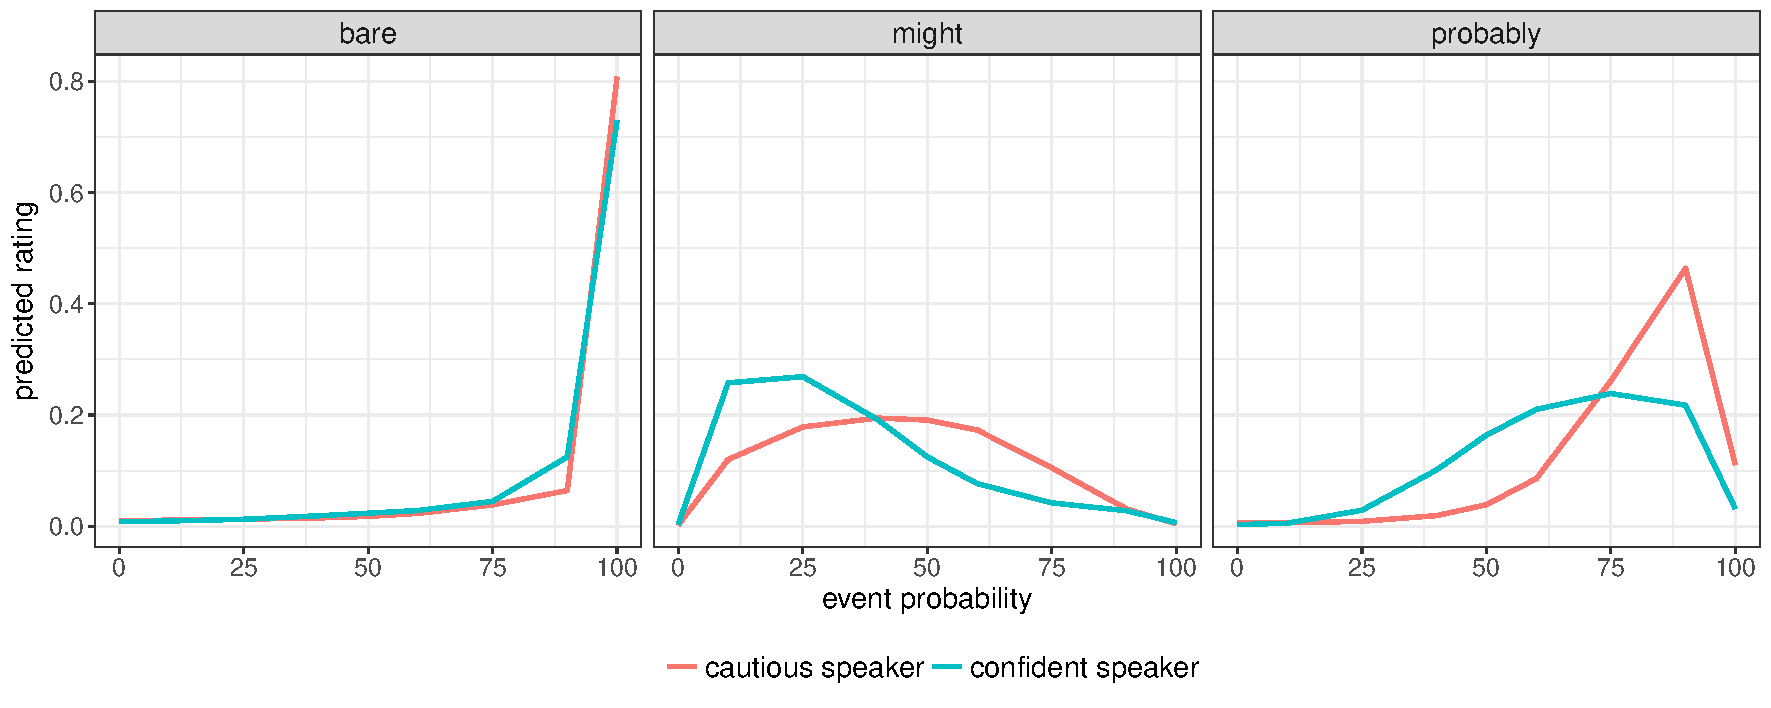
\includegraphics[width=\textwidth]{plots/adaptation-posterior-comp.pdf}
  \caption{Post-adaptation interpretation distributions for the utterances  \textsc{bare}, \textsc{might}, and \textsc{probably} as predicted by the pragmatic listener $L$\textsubscript{$1$}. \label{fig:post-exposure-comp}}
\end{figure}

Up to this point, we focused on listeners' expectations about a speaker's use of uncertainty expressions. As we discussed
in the introduction, we expect updated expectations to have an effect on the interpretation of uncertainty expressions. This
effect is also predicted by RSA models,  which assume that a pragmatic listener $L_1$ tries to infer the state of the world (in our case, the event probability $\phi$) by reasoning
about their prior beliefs about the world state and their expectations about a speaker's language use (in our case, the expected pragmatic speaker $ES_{1}$).

$$ L_1(\phi \mid u) \propto P(\phi) ES_1(u \mid \phi)$$

According to such a model of interpretation, the shifts in expectations that we observed in the previous experiment, should also lead to a shift in interpretations. 
If we again assume a uniform prior over event probabilities, then our model predicts that listeners who were exposed to a \textit{cautious} speaker should infer 
higher event probabilities when hearing {\sc might} or {\sc probably} than listeners who were exposed to a \textit{confident} speaker. Figure~\ref{fig:post-exposure-comp}
shows the distribution over event probabilities after hearing three different utterances as predicted by $L_1$ parameterized by the inferred parameters from our
adaptation simulations in the previous section. As these plots show, in the \textit{cautious speaker} condition, the distribution over event probabilities after hearing \textit{might} 
and \textit{probably} is shifted towards higher values as compared to the distributions in the \textit{confident speaker} condition. 

In this experiment, we tested whether this prediction is correct and whether listeners' change in expectations transfers to a change in interpretations. 
The procedure, materials and analyses were pre-registered at \url{https://osf.io/ghnc3}.

\subsection{Participants}

We recruited a total of 80 participants (40 per condition) on Amazon Mechanical Turk. We required participants to have a US-based IP address and a minimal approval rating of 95\%. Participants were paid \$1.5 which amounted to an hourly wage of approximately \$15. None of the participants had participated in any of the previous experiments. 

\subsection{Materials and Procedure}

Participants completed a set of exposure trials followed by a set of test trials. The exposure trials were identical to the exposure trials in Experiment~1b. The test trials probed participants' interpretations of the utterances {\sc might}, {\sc probably} and {\sc bare}. On each test trial, participants listened to a recording of the speaker from the exposure phase producing {\sc might}, {\sc probably} and {\sc bare} and then participants were asked to rate for 9 gumball machines with the same proportions of blue and orange gumballs as in the previous experiments how likely they thought it was that the speaker saw each of these gumball machines by distributing coins.  Participants 10 coins per trial and completed in total 6 trials -- one for each expression-color pair. The exposure phase contained again 6 attention check as in the previous experiment. However, given the low attention check performance in the previous experiments, we modified the attention checks. Instead of asking participants whether they saw an X on the previous trial, we asked participants to choose the gumball machine that they had seen on the previous trial among two machines displayed in random order.

\subsection{Exclusions}

We excluded participants who failed more than 2 attention checks, which led to 1 exclusion in the \emph{cautious speaker} condition and 1 exclusion in the \emph{confident speaker} condition.


\subsection{Analysis and Predictions}

If participants update their expectations of a specific speaker's use of uncertainty expressions,  we expect that listeners interpret a more confident speaker's utterance 
to communicate a lower event probability than a more cautious speaker's utterance. We tested this prediction by treating participant's distributions of coins 
of gumball machines as a probability distribution over gumball proportions (and consequently event probabilities).  For each utterance, we 
normalized participants' coin distributions such that they summed up to 1, so that we could interpret the normalized scores 
as a categorical probability distribution over gumball machines given an utterance. We computed the expected value of target color gumballs 
from these probability distributions and compared these expected values across the two conditions. We predicted that the expected values of 
{\sc might} and {\sc probably} would be larger in the \emph{cautious speaker} condition than in the \emph{confident speaker} condition.

\subsection{Results and Discussion}

\begin{figure}
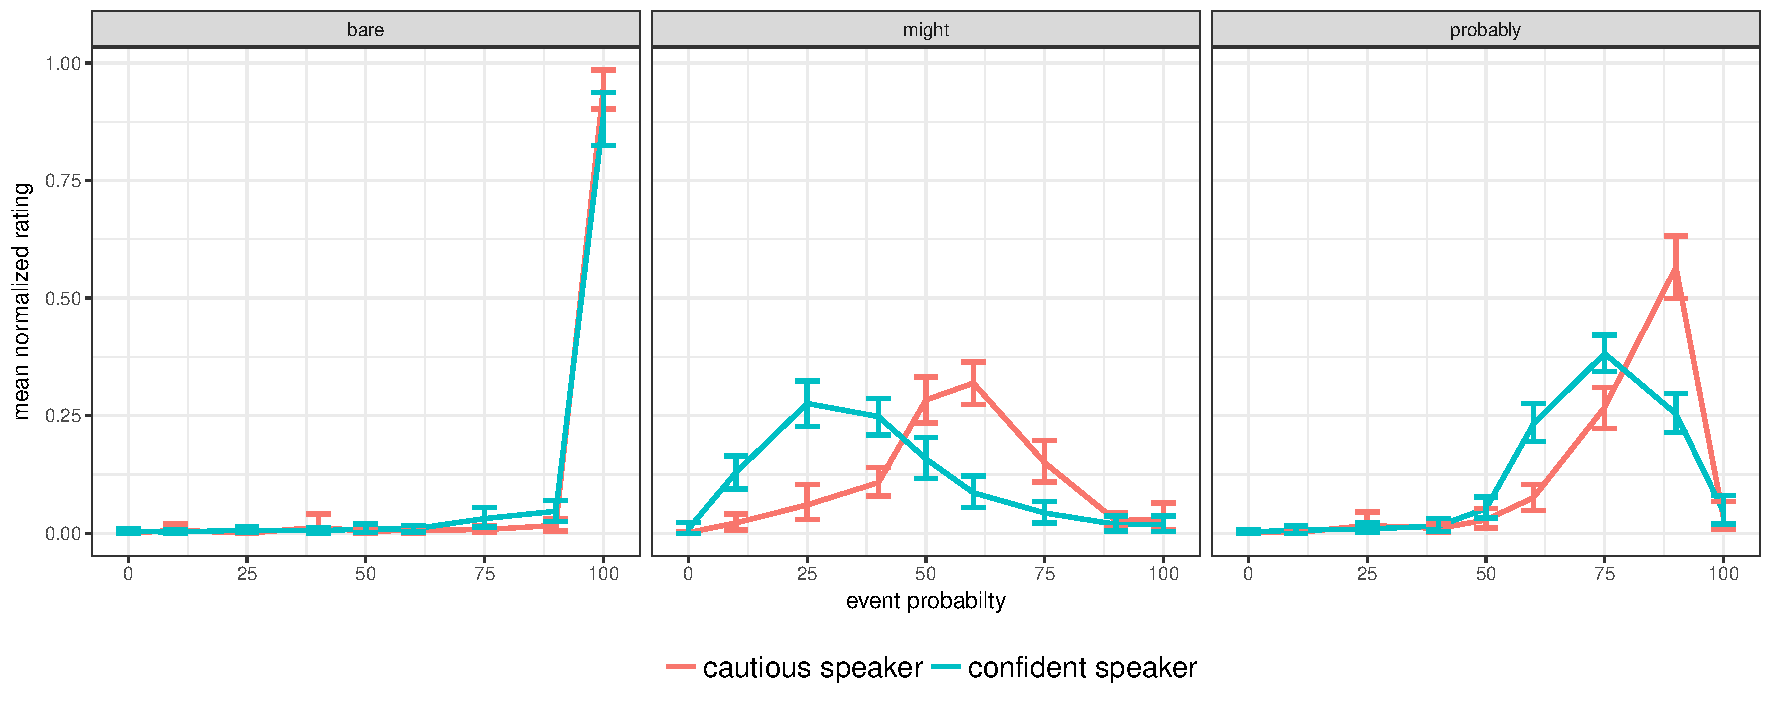
\includegraphics[width=\textwidth]{plots/exp-2-ratings.pdf}
\caption{Aggregated post-exposure ratings from Experiment~2. Error bars correspond to bootstrapped 95\%-confidence intervals.  \label{fig:adaptation-results-comp}}
\end{figure}

Figure~\ref{fig:adaptation-results-comp} shows the aggregated and normalized ratings for the two conditions.  As predicted, participants provided higher ratings for gumballs with higher target color percentages after hearing {\sc might} and {\sc probably} in the \emph{cautious speaker} condition than in the \emph{cautious speaker} condition. This also led to a significantly higher expected value for {\sc might} ($t(76)=5.84$, $p<0.001$) and {\sc probably} ($t(76)=3.92$, $p<0.001$) in the \emph{cautious speaker} condition as compared to the \emph{confident speaker} condition.

These results suggest that listeners not only update their expectations of what a speaker is likely to say in different situations but that also their interpretations of uncertainty expressions adapt to specific speakers.

\subsection{Model comparison}

\begin{table}
\center
\begin{tabular}{r | c | c }
Model & $R^2$ &   odds  \\ \midrule
fixed & 0.662 & $10^{-442}$    \\
cost & 0.885 &  $10^{-217}$  \\
threshold distributions & 0.888 & $10^{-116}$  \\
cost \& threshold distributions & 0.927 & 1 \\
\end{tabular}
\caption{Model evaluation results on data from Experiment~2.  $R$\textsuperscript{$2$} are computed between  the mean post-exposure ratings and the mean model predictions. \textit{odds} are the posterior likelihood odds of the models compared to the \textit{cost and threshold distributions} model.  \label{tbl:model-comparison-comp}}
\end{table}



We now return again to our main research question regarding the type of updated expectations. The production expectation experiments and model simulations provided strong evidence for listeners updating 
their beliefs about the threshold distributions. On the other hand, the two evaluation metrics provided conflicting results regarding the questions whether beliefs about speaker preferences are also updated.
We therefore also compared the pragmatic listener $L_1$ predictions from the simulations with different prior structures to the post-exposure ratings in Experiment~2. To this end, we took the
posterior distributions over model parameters that we obtained through the simulations in the previous section and computed the predictions of the $L_1$ model. \tableref{tbl:model-comparison-comp} shows the model fit
for the different types of simulations. As this table shows, the model according to which both threshold distributions and costs are being updated provides the best fit according to both metrics. 
Considering that the posterior likelihood odds consistently favored this model in all three model comparisons, we take these results together as strong evidence that listeners are updating their expectations about threshold distributions
and costs. 

\subsection{Model evaluation}
\begin{figure}
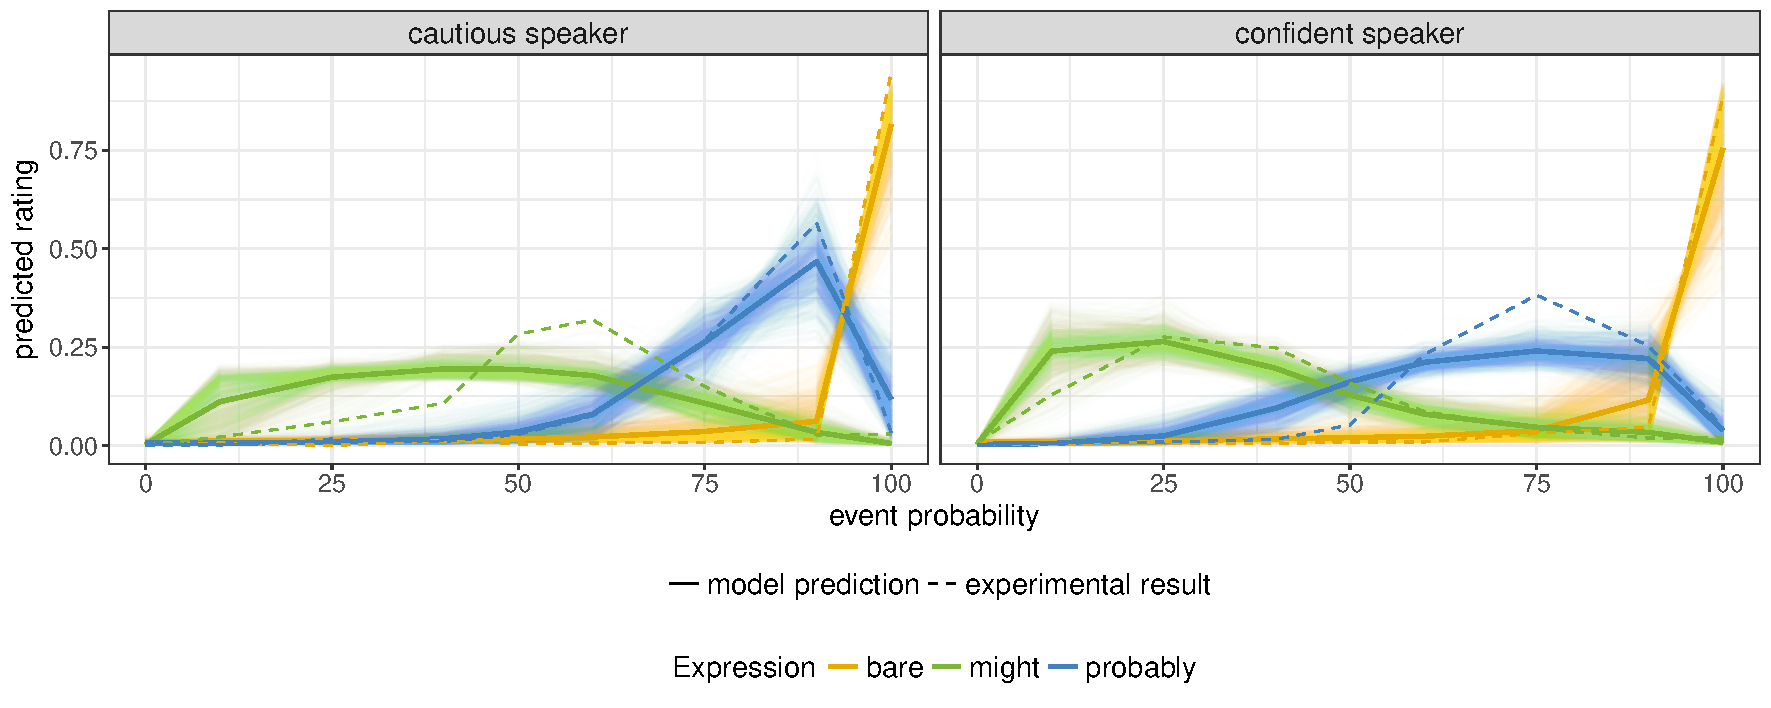
\includegraphics[width=\textwidth]{plots/adaptation-posterior-comp-data.pdf}
\caption{Predictions of \textit{threshold distributions and costs} model and data from Experiment~2. The shades around the mean indicate the distribution of model predictions.  \label{fig:post-exposure-comp-data}}
\end{figure}

\figref{fig:post-exposure-comp-data} superimposes the model predictions and the experimental data. As these plots show, the model makes both qualitatively and quantitatively accurate predictions for the interpretation of the \textsc{bare} utterance. The model further correctly predicts that participants expect the speaker to talk about relatively low event probabilities when hearing \textsc{might} in the \textit{confident speaker} condition, and it correctly predicts ratings of \textsc{probably} in the \textit{cautious speaker} condition. However, for the interpretation of \textsc{might} in the \textit{cautious speaker} condition, the model predicts a less peaked distribution than the empirical distribution and, to a lesser extent, the same is true for the interpretation of \textsc{probably} in the \textit{confident speaker} condition. We can only speculate about the reasons for this deviation but it could be that in these two cases, participants are considering alternative uncertainty expressions (e.g., \textit{very unlikely}) which we did not include in our model to be better descriptions for low event probabilities. If we added additional utterances to describe low probabilities to our model, it would correctly predict interpretation distributions that are more peaked at higher event probabilities. We leave a more detailed exploration of this issue to future work.

\section{General Discussion}

In two production expectation experiments (Experiments~1a and 1b), we found that listeners adapt to speakers who vary in their use of uncertainty expressions. This result confirms that 
the findings by \citet{Yildirim2016} also extent to the class of uncertainty expressions. In Experiment~2, we further found that adaptation has effects on the interpretation
of utterances, which had not been investigated before.

In a series of model comparisons, we found strong evidence for listeners updating their beliefs about the speaker's lexicon as well as the speaker's preferences, which suggests
that semantic/pragmatic adaptation is a result of updating both of these types of expectations. We further found that modeling the adaptation process as an instance of Bayesian
belief updating explains participants post-adaptation behavior well. Considering that belief updating models also explain adaptation results from other linguistic domains 
\citep[e.g.,][]{Kleinschmidt2012,Kleimschmidt2015,Roettger2019}, this potentially suggests that semantic/pragmatic adaptation is a result of cognitive processes that operate at all
linguistic levels.

More generally, our results also have important implications for theories about the lexicon. For content words such as nouns and verbs, it is generally assumed that 
the lexicon is highly dynamic and that listeners and speakers are able to compute novel senses on the fly \cite[e.g.,][]{Clark1983,ClarkGerrig1983,Griffiths2007?}. 
However, to the best of our knowledge, it was still an open question whether the meaning of function words such as uncertainty expressions is similarly dynamic.
Recent theoretical accounts of probability operators (a subset of uncertainty expression) \cite[e.g.,][]{Yalcin2010,Lassiter2016} hypothesized that the meanings of 
these expressions are highly dynamic and largely determined by the context. We provide a first \todo{is this true?} empirical validation of this hypothesis.





\begin{itemize}
\item Semantic/pragmatic adaptation is a result of listeners updating beliefs about the lexicon and speaker preferences
\item Bayesian-belief updating captures adaptation behavior well
\item Suggests that lexicon is more flexible than usually assumed (very much compatible with Lassiter, 2016; Bergen et al, 2016; Hawkins et al. 2017, Clark \& Gerrig, 1983, Clark 1983, Griffiths et al. 2007, ) -- BUT novel result that this is also the case for function words; primarily assumed for content words in the past


\item Consequences for mechanistic accounts: seems compatible with horton \& gerrig; associative vs. error correction (still unclear from these results)
\item Ecological validity? not fully interactive, and listeners observe world states. but presumably still ok
\item Open questions:
\begin{itemize}
\item Adapting to multiple speakers: preliminary results in Schuster and Degen, 2019
\item More exposure should lead to more adaptation: also preliminary evidence in Schuster and Degen, 2019
\item current experiments suggest rather dumb mechanism: listeners are tracking co-ocurrence statistics and 
are making inferences about the lexicon and preferences based on that -- seems unlikely that this is the full picture and
presumably listeners are also able to make more complex inferences; explaining away!
\end{itemize}
\end{itemize}


{\bf TODO} 

* talk about findings

provides evidence that bayesian belief updating is also a suitable model for higher-level linguistic tasks
priors are important




* contributions
	
	* marrying RSA with speaker-specific beliefs
	
	 * paradigm for studying uncertainty expressions
	
	 * latent semantics approach

 	 * dealing with uncertainty doesn't only seem to be true for lower-level processing but also higher-level processing
	 
	  * fits right into all the literature about language processing
	
	other things:
	
	*  memory mechanisms unclear but seems compatible with Horton \& gerrig and other memory processes
	
	* question about associative memory vs. error correction (still unclear) (look again at Brown-schmidt)
	
 	*  our approach similar to hawkins2017 and bergen, levy \& goodman
	
	*  relationship to pogue et al.
	
	*  discuss the unnatural nature of our experiment --$>$ not interactive (common in reading, news, ....); observed both world state
	     and the utterance --$>$ admittedly slightly unnatural but could be that one reads the weather report later or that people keep track
	     over time how likely events following what a person said
	     
       * wittenberg


future directions:

* talk about adaptation to multiple speakers

* talk about testing other predictions about the model

* long-term speaker-specific mappings
	
\todo{Speaker-specific}


\printbibliography
%\bibliography{qp-references}


%=====================================================================

%\begin{addresses}
 % \begin{address}
%    Author1 \\
%    Street \\
%    \ldots \\
%    \email{author1@email}
%  \end{address}
%  \begin{address}
 %   Author2 \\
 %   Street \\
 %   \ldots \\
 %   \email{author2@email}
 % \end{address}
 % ...
%\end{addresses}

%=====================================================================


\section*{Supplementary material}

\subsection*{Effect of color in norming study}

As mentioned in a footnote, we ran the norming studies in three batches using three slightly different procedures across conditions. We originally ran condition 0 (\emph{bare-might}) as a pilot condition. In the results, we noted that participants did not differ in their ratings depending on whether the girl asked for a blue or an orange gumball ($R^2(27)=0.997$ between mean ratings for blue and orange trials). To lower the number of trials, we therefore asked each participant to provide ratings for only one of the two colors (randomized across participants) for the next batch of conditions (conditions 1-14). We found that in some conditions, this led to small differences in ratings between participants who always rated utterances with \emph{blue} and participants who always rated utterances with \textit{orange} ($R^2(27)$ between $0.864$ and $0.984$). We hypothesize that this is a result of participants paying less attention if they were asked to do exactly the same task over and over again (in condition 0, the color potentially changed across trials). In order to verify the stability of our results, we replicated one of the conditions, condition 5 (\emph{might-probably}), and had participants provide two ratings for each color and gumball proportion. We found that despite the lower correlation between average ratings for utterances with \emph{blue} and utterances with \emph{orange} in the original run ($R^2(27)=0.929$), there was a very high correlation between the average ratings independent of the color of the original study and the average ratings of the replication ($R^2(27)=0.975$), which suggests that the average ratings largely do not depend on whether we ask participants to provide ratings for both colors or just one color. Nevertheless, we used the modified procedure in which we asked participants to provide 2 ratings for each color and gumball proportion for the last batch of conditions (conditions 15-20). In all conditions in which we asked people to provide ratings for utterances with both colors, the correlation between average ratings for utterances with \emph{blue} and utterances with \emph{orange} was almost perfect ($R^2(27)>0.988$).

\subsection*{Additional pre-exposure ratings}

\begin{figure}
\includegraphics[width=\textwidth]{plots/pre\string_test\string_s1.pdf}
\caption{Results of norming study -- Part 1. Error bars correspond to bootstrapped 95\%-confidence intervals. \label{fig:norming-results-1}}
\end{figure}

\begin{figure}
\includegraphics[width=\textwidth]{plots/pre\string_test\string_s2.pdf}
\caption{Results of norming study -- Part 2. Error bars correspond to bootstrapped 95\%-confidence intervals. \label{fig:norming-results-2}}

\end{figure}

\begin{figure}
\includegraphics[width=\textwidth]{plots/pre\string_test\string_model\string_s1.pdf}
\caption{Model predictions and results from norming study -- Part 1. Error bars correspond to 95\% high density intervals (model predictions) and bootstrapped 95\%-confidence intervals (observed results). \label{fig:norming-results-model-1}}

\end{figure}

\begin{figure}
\includegraphics[width=\textwidth]{plots/pre\string_test\string_model\string_s2.pdf}
\caption{Model predictions and results from norming study -- Part 2. Error bars correspond to 95\% high density intervals (model predictions) and bootstrapped 95\%-confidence intervals (observed results). \label{fig:norming-results-model-2}}

\end{figure}

\subsection*{Original interpretation experiment}

\todo{Revise this section}

\subsection{Participants}

We recruited a total of 80 participants (40 per condition) on Amazon Mechanical Turk. We required participants to have a US-based IP address and a minimal approval rating of 95\%. Participants were paid \$2 which amounted to an hourly wage of approximately \$10--\$12. None of the participants had participated in any of the previous experiments. 

\subsection{Materials and Procedure}

Participants completed a set of exposure trials followed by a set of test trials. The exposure trials were identical to the exposure trials in Experiment~1. The test trials probed participants' interpretations of the utterances {\sc might}, {\sc probably} and {\sc bare}. In each test trial, participants listened to a recording of the speaker from the exposure phase producing {\sc might}, {\sc probably} and {\sc bare} and then participants were asked to rate for 9 gumball machines with the same proportions of blue and orange gumballs as in the previous experiments how likely they thought it was that the speaker saw each of these gumball machines by adjusting a slider. All 9 gumball machines were presented at the same time but to avoid visual clutter, all gumball machines except the one whose slider participants were adjusting had an opacity of 0.1 and the animation was disabled. Participants provided 9 ratings per trial and completed in total 6 trials -- one for each expression-color pair. The exposure phase contained again 6 attention check as in the previous experiment. However, given the low attention check performance in the previous experiment, we modified one aspect about the attention checks: We always displayed the grey X on the first trial with an attention check so that participants would see the gray X before being presented with the attention check. We discarded answers to the first attention check and computed the attention check performance on the remaining 5 attention checks.

\subsection{Exclusions}

We excluded participants who failed more than 2 attention checks, which led to 2 exclusions in the \emph{cautious speaker} condition and 1 exclusion in the \emph{confident speaker} condition.


\subsection{Analysis and Predictions}

If participants reason about the speaker and update their expectations of a specific speaker, we also expect that participants interpretations 
vary depending on which speaker they were exposed to. Concretely, we expect that listeners interpret a more confident speaker's utterance 
to communicate a lower event probability than a more cautious speaker's utterance. We tested this prediction by treating participant's ratings 
of gumball machines as a probability distribution over gumball proportions (and consequently event probabilities).  For each utterance, we 
normalized participants ratings of the different gumball machines so that they summed up to 1, so that we could interpret the normalized scores 
as a categorical probability distribution over gumball machines given an utterance. We computed the expected value of blue gumballs from these probability distributions and compared these expected values across the two conditions. We predicted that the expected values of {\sc might} and {\sc probably} were going to be larger in the \emph{cautious speaker} condition than in the \emph{confident speaker} condition.

\subsubsection{Results and Discussion}

\begin{figure}
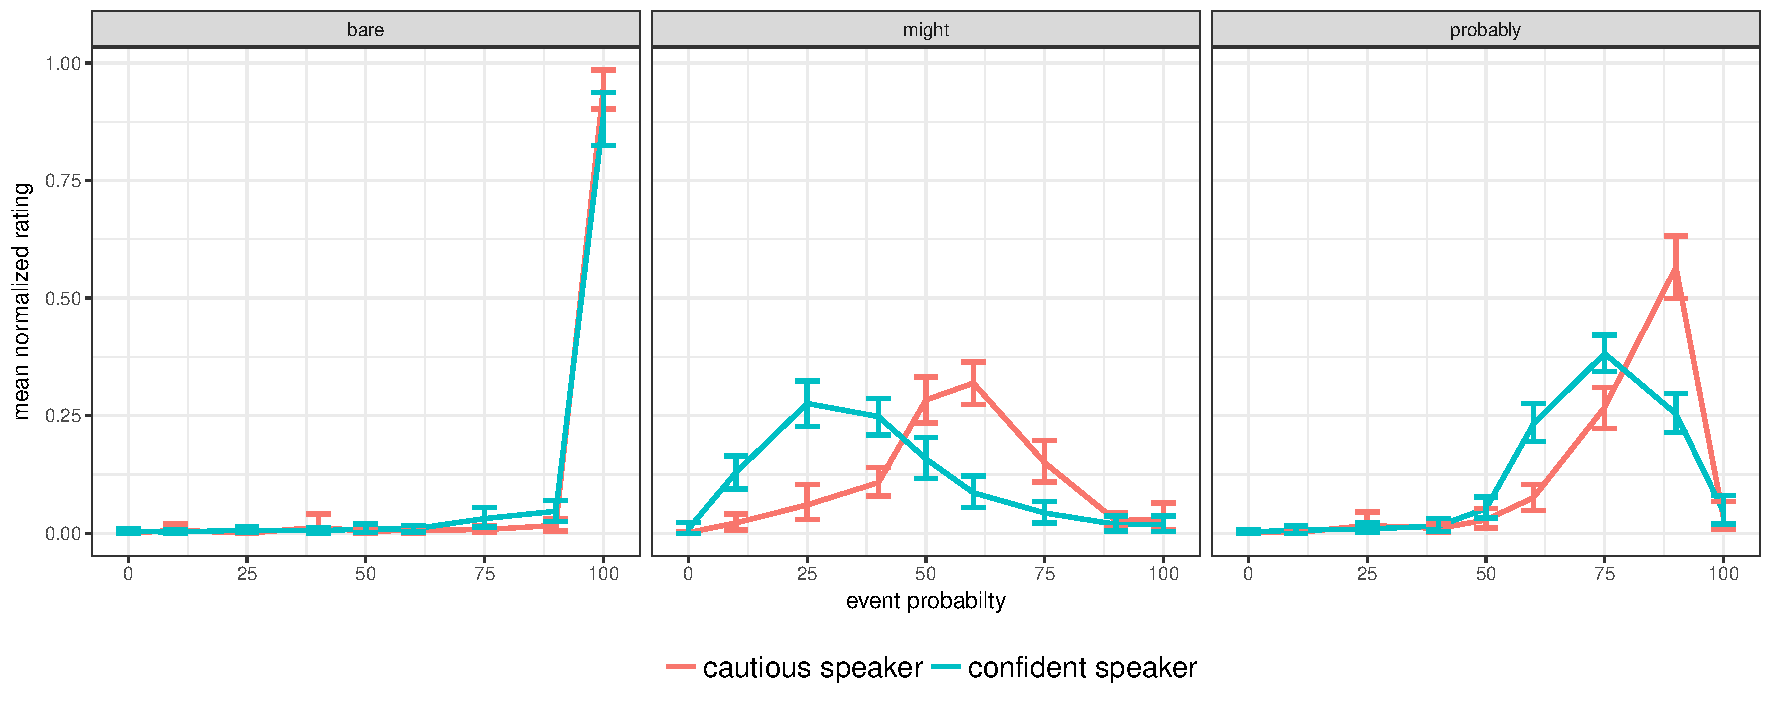
\includegraphics[width=\textwidth]{plots/exp-2-ratings.pdf}
\caption{Aggregated post-exposure ratings from Experiment~2.  \label{fig:adaptation-results-comp}}
\end{figure}

\begin{figure}
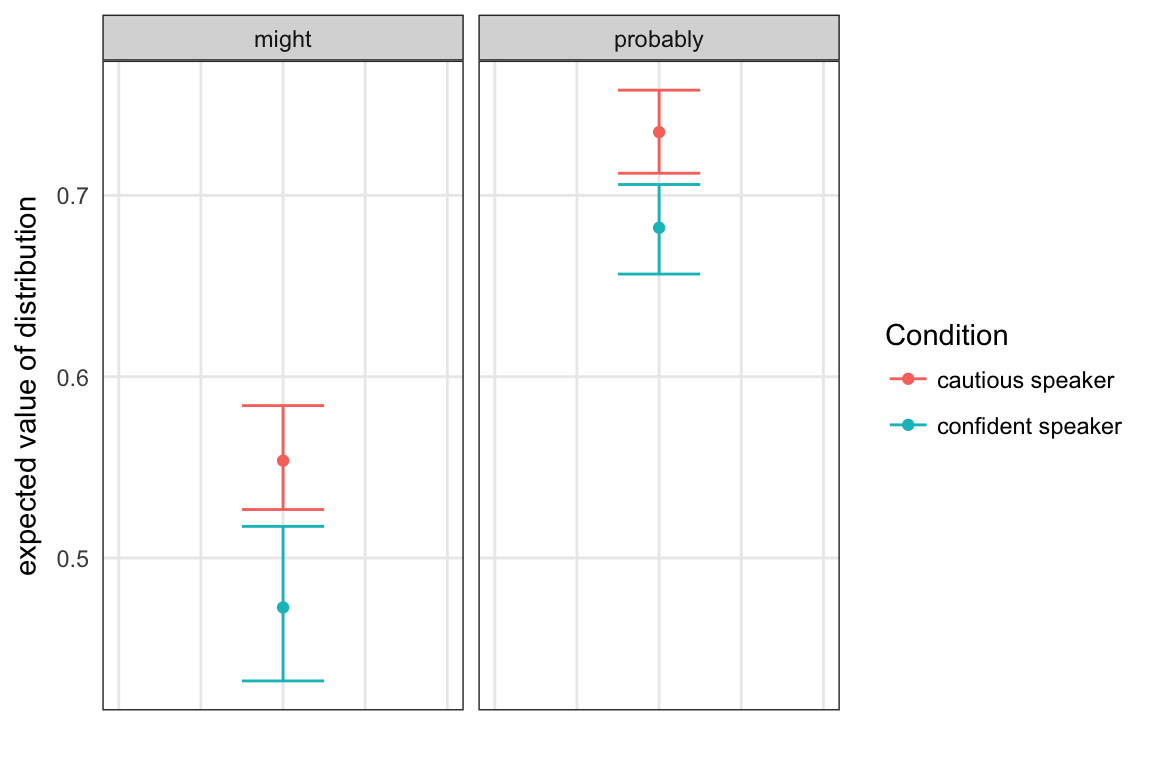
\includegraphics[width=.75\textwidth]{plots/adaptation-diff-comprehension.png}
\caption{Expected values for {\sc probably} and {\sc might} from Experiment~2.  \label{fig:adaptation-exp-comp}}
\end{figure}


Figure~\ref{fig:adaptation-results-comp} shows the aggregated and normalized ratings for the two conditions.  As predicted, participants provided higher ratings for gumballs with higher target color percentages after hearing {\sc might} and {\sc probably} in the \emph{cautious speaker} condition than in the \emph{cautious speaker} condition. This also led to a significantly higher expected value for {\sc might} ($t(75)=3.05$, $p<0.01$) and {\sc probably} ($t(75)=3.08$, $p<0.01$, see also Figure~\ref{fig:adaptation-exp-comp}) in the \emph{cautious speaker} condition as compared to the \emph{confident speaker} condition.

These results suggest that listeners not only update their expectations of what a speaker is likely to say in different situations but that also their interpretations of uncertainty expressions adapt to specific speakers.



%\section{Models}
%
%While the results of the two experiments suggest that there is considerable variation in the use of uncertainty expressions and that listeners can adapt their speaker expectations after listening to a speaker several times, the experimental results do not explain the adaptation process. We therefore also attempt to model participant behavior using a Bayesian cognitive model. In particular, we are investigating whether adaptation is a result of participants learning the speaker's  utterance {\bf preferences}, learning the speaker's {\bf meanings} of uncertainty expressions (i.e., which range of probabilities does an uncertainty expression map to in this specific context) or a combination of learning speaker {\bf preferences} and {\bf meanings}.
%
%\subsection{Overview}
%
%We model adaptation as Bayesian belief updates about the {\bf meanings} of uncertainty expressions and utterance {\bf preferences}. Formally, let $\Theta_S$ be the set of parameters that governs the meaning of uncertainty expressions used by speaker $S$ as well as the utterance preferences by $S$. We assume that a listener updates their beliefs about $\Theta_S$ after hearing a specific speaker produce utterances with uncertainty expressions along with observations that allow the listener to infer the probability of an event happening, i.e., after experiencing set $\mathscr{D}$ of $(u, \phi)$ observations, a listener updates their beliefs about $\Theta_S$\footnote{Similar models have also been proposed by \cite{Qing2013} and \cite{Hawkins2017} for adaptation to different uses of quantifiers and convention formation, respectively.}:
%
%$$P(\Theta_S \mid \mathscr{D}) \propto P(\Theta_S) P(\mathscr{D} \mid \Theta_S) = P(\Theta_S) {\textstyle \prod_{(u, \phi) \in \mathscr{D}} } S_1(u \mid \phi; \Theta_S).$$
%
%\noindent Here, we assume that the likelihood of the set of observations $\mathscr{D}$ is the likelihood of producing utterances $u$ given an event probability $\phi$ according to a speaker model $S_1$ parametrized by $\Theta_S$. We now discuss both this speaker model $S_1$ as well as the prior distribution $P(\Theta_S)$ in turn.
%
%\subsection{Speaker-specific production and comprehension model}
%
%We model production and comprehension within the Rational Speech Act (RSA) framework \citep{XXX}. We follow previous work on uncertainty expressions \citep{Lassiter2013,Herbstritt2017} and assume that uncertainty expressions have a threshold semantics, i.e., an utterance with an uncertainty expression  $u$  is semantically felicitous if it denotes a proposition that has probability $\phi$, which exceeds a threshold $\theta_u$:
%
%$$L_0(\phi \mid u, \theta_u) \propto P(\phi) \times \mathbbm{1}\left[\phi > \theta_u\right]$$ 
%
%A pragmatic speaker $S_1$ (our production model) then chooses her utterance to communicate that an event will happen with probability $\phi$ by soft-maximizing her speaker utility 
%$$EU_S(\phi, u) =  \int_0^1 {P_S\left(\theta_U\right) \log L_0(\phi \mid u, \theta_u) d\theta - c_S(u) },$$ which is the difference of the negative surprisal of the listener and the speaker-specific utterance cost $c_S(u)$.  Here, we also assume that in choosing an utterance, a speaker samples a threshold $\theta_u$ from probability distributions $P_S\left(\theta_u\right)$ which represent $S_1$'s beliefs about reasonable thresholds.
%
%
%$$S_1(u \mid \phi) \propto   \exp \lambda U_S\left(\phi, u \right),$$
%
%\noindent where $P_S(\theta) = \prod_{u \in U}P_S(\theta_u)$ and $\lambda$ is a rationality parameter which governs the optimality of the speaker choice. A pragmatic listener $L_1$ (our comprehension model)  interprets these utterances by reasoning about the speaker:
%
%$$L_1(\phi \mid u) \propto P(\phi) S_1(u \mid \phi).$$
%
%\noindent Our speaker-specific model crucially depends on two speaker-specific functions, namely the distributions over thresholds $P_S(\theta_u)$ and the cost function $c_S(u)$. We assume that each $P_S(\theta_u)$ follows a Beta distribution with parameters $\alpha_{Su}$ and $\beta_{Su}$. Beta distributions seem well-suited for two reasons: First, $\theta_u$ always has to be within the interval $[0,1]$, which is identical to the support of a Beta distribution, and second, Beta distributions can take many different shapes and we expect that for some uncertainty expressions, most of the probability mass is concentrated at one of the endpoints. For the cost function, we assume that a speaker's utterance cost is a constant depending on the uncertainty expression $c_S(u)=\gamma_{Su}$. The utterances that we are considering are all of approximately equal length, so we assume that the cost term primarily captures speaker preferences rather than processing costs. 
%
%\subsection{Priors}
%
%Adult listeners are experts in language use in their native language and hence we expect them to have very strong prior expectations on how speakers use language. We encode this prior knowledge in the prior $P(\Theta_S)$. We assume that this prior is the joint probability of all parameters in $\Theta_u$, which we assume to be independent. Beta distributions can be parametrized in numerous ways (see e.g., \cite{Kruschke2014}) which can make inference easier or harder  and avoid potentially degenerate solutions. For adaptation, we reparameterize the Beta distributions over thresholds $\theta_{Su}$ using the distribution mean $\mu= \frac{\alpha}{\alpha + \beta}$ and the population size parameter $\nu=\alpha + \beta$. We assume that the prior parameters follow the following distributions:
%
%$$\mu_u \sim \mbox{TruncatedNorm}(\mu_{\mu_u}, \sigma_{\mu_u}, 0, 1) \qquad \nu_u \sim \mbox{Log-Norm}(\mu_{\nu_u}, \sigma_{\nu_u}) $$
%$$ \gamma_u \sim \mbox{Log-Norm}(\mu_{\gamma_u}, \sigma_{\gamma_u})$$
%
%$\mu_u$ always has to be within the interval $[0,1]$ and within that it seems to roughly follow a Normal distribution, therefore we opted for a truncated normal as a prior for these parameters. $\nu_u$ and $\gamma_u$ on the other hand, always have to be greater than 0 and a log-normal distribution seems to describe the distribution of parameters very well.
%
%\subsubsection{Mean estimation}
%
%We estimated the parameters for the prior as well as the rationality parameter $\lambda$ from the norming study using Bayesian data analysis. We treated each participants rating over utterances in a trial as a probability distribution over utterances given an event probability $\phi$ and we sampled 10 utterances from each of these distributions, resulting in a set $\mathscr{E}$ of utterance/probability pairs $(u, \phi)$. We then estimated the means of the prior distributions over parameters $\theta_S$, i.e., $\mu_{\mu_u}$, $\mu_{\nu_u} $  and $\mu_{\gamma_u}$ for each utterance $u$ by estimating the MAP values of the posterior distribution 
%
%$$P(\theta_S, \lambda \mid \mathscr{E}) = P(\theta_S, \lambda) P(\mathscr{E} \mid \theta_S, \lambda) = P(\theta_S, \lambda) \prod_{(u,\phi) \in \mathscr{E}} S_1'(u \mid \phi, \theta_S, \lambda).$$ 
%
%$S_1'$ is a modified version of the speaker-specific production model $S_1$ which makes a few additional assumptions with respect to the data collection.
%
%\begin{enumerate}
%\item Instead of $c(u)$, we use a special condition-specific cost function:
%$$
%c(u, condition) = 
%     \begin{cases}
%       0 &\quad\text{if } u  \text{ is one of the utterances in } condition\\
%       \gamma &\quad\text{otherwise} \\
%     \end{cases}
%$$
%\item We include a noise term and we assume that in 5\% of the cases participants chose a random utterance.
%\item We assume the set of possible utterances is comprised of the seven utterances with uncertainty expressions that we mentioned above, i.e., $U = \{$ {\sc bare}, {\sc might}, {\sc probably}, {\sc could}, {\sc think}, {\sc looks like}, {\sc bare not}$\}$
%\item We assume that $$S_1'(\mbox{\textit{``other''}} \mid \phi, \mbox{condition}) \propto O + \sum_{u \in U \land u \not \in \mbox{condition}} S_1(u \mid \phi)$$
%\item Speaker-specific parameters $\Theta_S$ are shared across all participants.
%\end{enumerate}
%
%The rationale behind assumption (i) is that we only provide participants with two utterance choices and the blanket \emph{other} response in the norming study and therefore we expect that participants will be heavily primed to use the two provided utterances whenever they are semantically felicitous, which we can model with our condition-specific cost function. Also note that we assume that all utterances have the same cost  $\gamma$ if they are not part of the current condition. We made this choice based on the finding that the model tended to overfit the data when we allowed each of these parameters to vary independently, and as mentioned earlier, given that all the utterances have approximately the same length, we don't expect that participants have strong expectations about the preferences of a speaker a priori to encountering the actual speaker. 
%
%The rationale behind assumption (ii) is that as in any web-based experiment, we will have participants who make random choices, do not pay attention, or make mistakes, and we do not want that noise to influence our actual parameter estimation. This is in particular important for expressions that tend to have very high thresholds $\theta_u$. For example, a rational participant who pays attention is highly unlikely to assign a rating above 0 to the utterance ``You'll get a blue one'' if the objective probability of getting a blue gumball is 0\% and we want this to be reflected in our distribution $P\left(\theta_{\mbox{bare}}\right)$. However, if a few participants who either did not pay attention or made mistakes provide non-zero ratings for this utterance/probability combination, this could skew the threshold distribution considerably towards 0, which is something we want to avoid.
%
%The reason for assumption (iii) is that we only collected data for this set of utterances and that the RSA model the way we specified here requires a fixed set of utterances.
%
%Finally, in our experiments, participants cannot freely choose among all utterances that they would be able to produce in a more naturalistic setting. We therefore assume that they reason about other utterances which include the 5 utterances that were not part of the respective condition as well as other utterances that we are not even considering here. This is captured by the fact that we are summing over all the other utterances and an inferred constant $O$, which is intended to capture the probability of all utterances that we didn't consider in any of the conditions.
%
%
%
%\subsubsection{Variance estimation}
%
%\subsubsection{Implementation details}
%
%We implemented the model in Python using {\tt numpy} and {\tt scikit-learn} libraries. We used MCMC with the  Metropolis-Hastings algorithm. For the MAP estimation, we collected 100,000 MCMC samples after discarding the first 20,000 burn-in samples. This samples were obtained by collecting  a sample at every 10th iteration (i.e., we used thinning of 10). For the bootstrapping procedure, we collected 20,000 MCMC samples of each run and discarded the first 10,000 burn-in samples. Again, we thinned the chain by collecting samples at every 10th iteration. 
%
%We used the following proposal distributions for the various parameters:
%
%$$\alpha_u^{(t)} \sim \mbox{Log-Norm}(\alpha_u^{(t-1)}, XXX) $$
%$$\beta_u^{(t)} \sim \mbox{Log-Norm}(\beta_u^{(t-1)}, XXX)  $$
%$$\gamma^{(t)} \sim \mbox{Log-Norm}(\gamma^{(t-1)}, XXX)$$
%$$\lambda^{(t)} \sim \mbox{Uniform}(\lambda^{(t-1)}-XXX, (\lambda^{(t-1)}+XXX)$$
%
%
%Uninformed priors. 
%
%\subsubsection{Inferred parameters}
%
%\subsubsection{Model predictions and criticism}
%
%
%
%\subsection{Pre-test experiment}
%
%\subsubsection{Model}
%
%We model the process that leads to the experimental results in the pre-test experiment as a speaker model ($S_1$) in the Rational Speech Acts framework \citep{RSA}. We assume that participants take the role of a generic speaker but given that they reason about a non-specific speaker, participants have some uncertainty about the speaker's language use.
%
%Within the RSA framework, a pragmatic speaker reasons about a literal listener ($L_0$). In the context of our experiment, we define the following literal listener in a similar vain as Lassiter and Goodman (2015) and Herbstritt and Franke (2017). 
%$$L_0(\phi \mid u; \theta) \propto P(\phi) \left( {0.95} \times \mathbbm{1}[\phi > \theta_{u}] + 0.05 * P_{uniform}(\phi; 0,1) \right)$$
%
%The literal listener tries to infer the probability $\phi$ of an event happening (in our case, the probability of getting a blue gumball) from an utterance with an uncertainty expression $u$. We assume that for each uncertainty expression, there is some threshold $\theta_u$ such that $u$ is semantically felicitous if  $\phi$ is above this threshold. We assume that the prior $P(\phi)$ is uniform. Given that we are dealing with noisy experimental data, we also include a noise term of the form $0.05 * P_{uniform}(\phi; 0,1)$, which allows for random inferences in 5\% of the cases. 
%
%\vspace{1em}
%
%\textbf{Q:} Is this a reasonable way to model noise?
%
%\vspace{1em}
%
%
%We assume that each uncertainty expression has its own threshold, except for the negated version of the bare statement, which we assume to be true if $\phi$ is less than $1-\theta_{bare}$ (Herbstritt and Franke, 2017).
%
%Given this literal listener, a pragmatic speaker $S_1$, tries to maximize the listener's utility when choosing an utterance to communicate the probability $\phi$. We assume that a speaker chooses among the 6 utterances that were used across the 15 conditions and the the negated version of the bare statement, i.e., \textit{"You won't get a blue one"}.
%$$S_1( u \mid \phi, condition; \theta ) \propto exp \left(\lambda \left( \log P_L(\phi \mid u; \theta) - c(u, condition) \right) \right) $$
%
%Following the vanilla RSA model, we define the utility as the negative surprisal subtracted by the cost of the utterance. Given our experimental setting in which we ask participants to choose between two given utterances and \textit{other}, we use the following cost function, which depends on the experimental condition.
%$$
%c(u, condition) = 
%     \begin{cases}
%       0 &\quad\text{if } u  \text{ is one of the utterances in } condition\\
%       c_{u} &\quad\text{otherwise} \\
%     \end{cases}
%$$
%
%The motivation here is that participants will be primed to use the two given utterances, which is reflected in the lower cost.
%
%The $S_1$ model that we presented here is still parameterized by a set of thresholds $\theta$. Considering the variation in use of uncertainty expressions, participants seem to show uncertainty about how a generic speaker would set $\theta$ for the individual uncertainty expressions. We therefore assume that participants come with a prior over reasonable thresholds and given that they are asked to reason about an unknown speaker, they marginalize over this prior to derive the distribution over utterances, which results in the following revised speaker model.
%
%$$P_S(u \mid \phi, condition) \propto \int P(\theta) exp\left(\lambda  \left(\log P_L(\phi \mid u; \theta) - c(u, condition)\right)\right) d\theta $$
%
%\subsubsection{Parameter estimation}
%
%Our model has 14 parameters, namely 6 prior distributions over thresholds $P(\theta_u)$, 7 cost terms $c_u$, and the rationality parameter $\alpha$, which we all estimate from the experimental data. For the prior distributions $P(\theta_u)$, we assume that these follow a beta distribution parametrized by $\alpha_u$ and $\beta_u$ (Qing (2014) made similar assumptions for modeling the use of \textit{some} and \textit{many}). There are two main reasons for choosing a beta distribution: First, its range is from 0 to 1, and given that $\theta$ defines a threshold parameter for a probability, this matches exactly the reasonable interval for the thresholds. Second, the beta distribution can take very different shapes and therefore we are not making the assumption that all of the prior distributions over thresholds have a similar shape.
%
%To facilitate computations, we discretize our speaker and listener model as well as the priors over thresholds and infer these distributions by enumerating all possibilities. To estimate the model parameters, we run MCMC with 8,000 burn-in samples and 12,000 samples.\footnote{Note that this does not seem to be enough samples yet as 3 different runs still lead to varying results and don't pass the criterion by Gelman and Rubin (1992). I'm currently running the model again with 100,000 samples, which will hopefully be enough for stable parameter estimates.} 
%
%We sample parameters from the following distributions.
%
%$$\alpha_u, \beta_u \sim Uniform(0,30)$$
%$$c_u\sim Uniform(0,5)$$
%$$\lambda \sim Uniform(0.1,3)$$
%
%We then estimate the parameters by computing the distributions over parameters given the experimental data across all 15 conditions $\mathscr{D}$.
%
%\begin{align*}
%P(\alpha,\beta, c, \lambda \mid \mathscr{D}) &\propto P(\alpha, \beta, c, \lambda) P(\mathscr{D} \mid \alpha,\beta, c, \lambda) \\
%&= P(\alpha, \beta, c, \lambda) \prod_{d \in \mathscr{D}} P_S(u_d \mid \phi_d, condition_d; \alpha, \beta, c, \lambda)
%\end{align*}
%
%Note that for each probability $\phi$, participants provided a distribution over utterances and not actual samples of utterances given $\phi$. For each trial in which a participant provided a distribution over utterances, we therefore sampled 10 utterances from this distribution and combined all of these samples to form the data $\mathscr{D}$ from which we estimated the parameters of our model.
%
%For each parameter, we take the median of the 12,000 MCMC samples and use these parameter estimates for making model predictions.
%
%
%\subsubsection{Model predictions}
%
%The following plots show the experimental results (left) and the model predictions (middle) for several (representative) conditions.\footnote{See \url{https://github.com/sebschu/adaptation/blob/master/models/1_threshold_modals/prediction_model.html} for results for all 15 conditions.}
%
%\begin{center}
%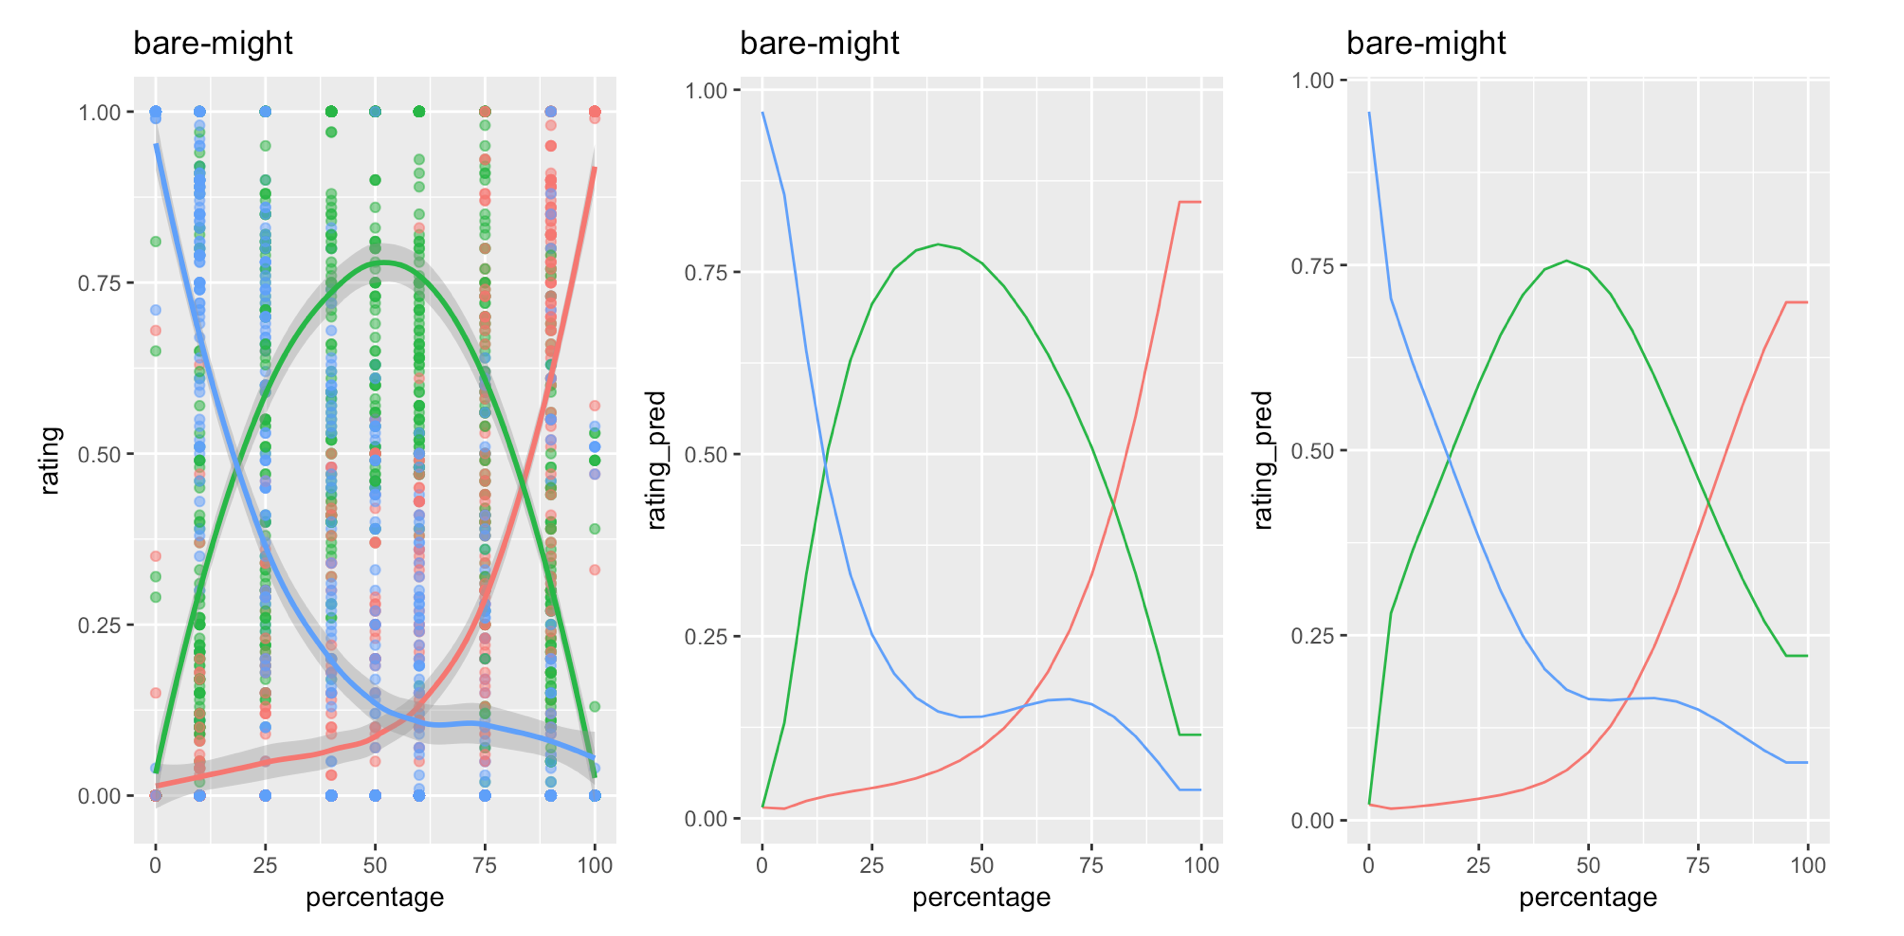
\includegraphics[width=\textwidth]{plots/bare-might-predictions.png} \\
%bare (red) - might (green) condition
%
%\vspace{2em}
%
%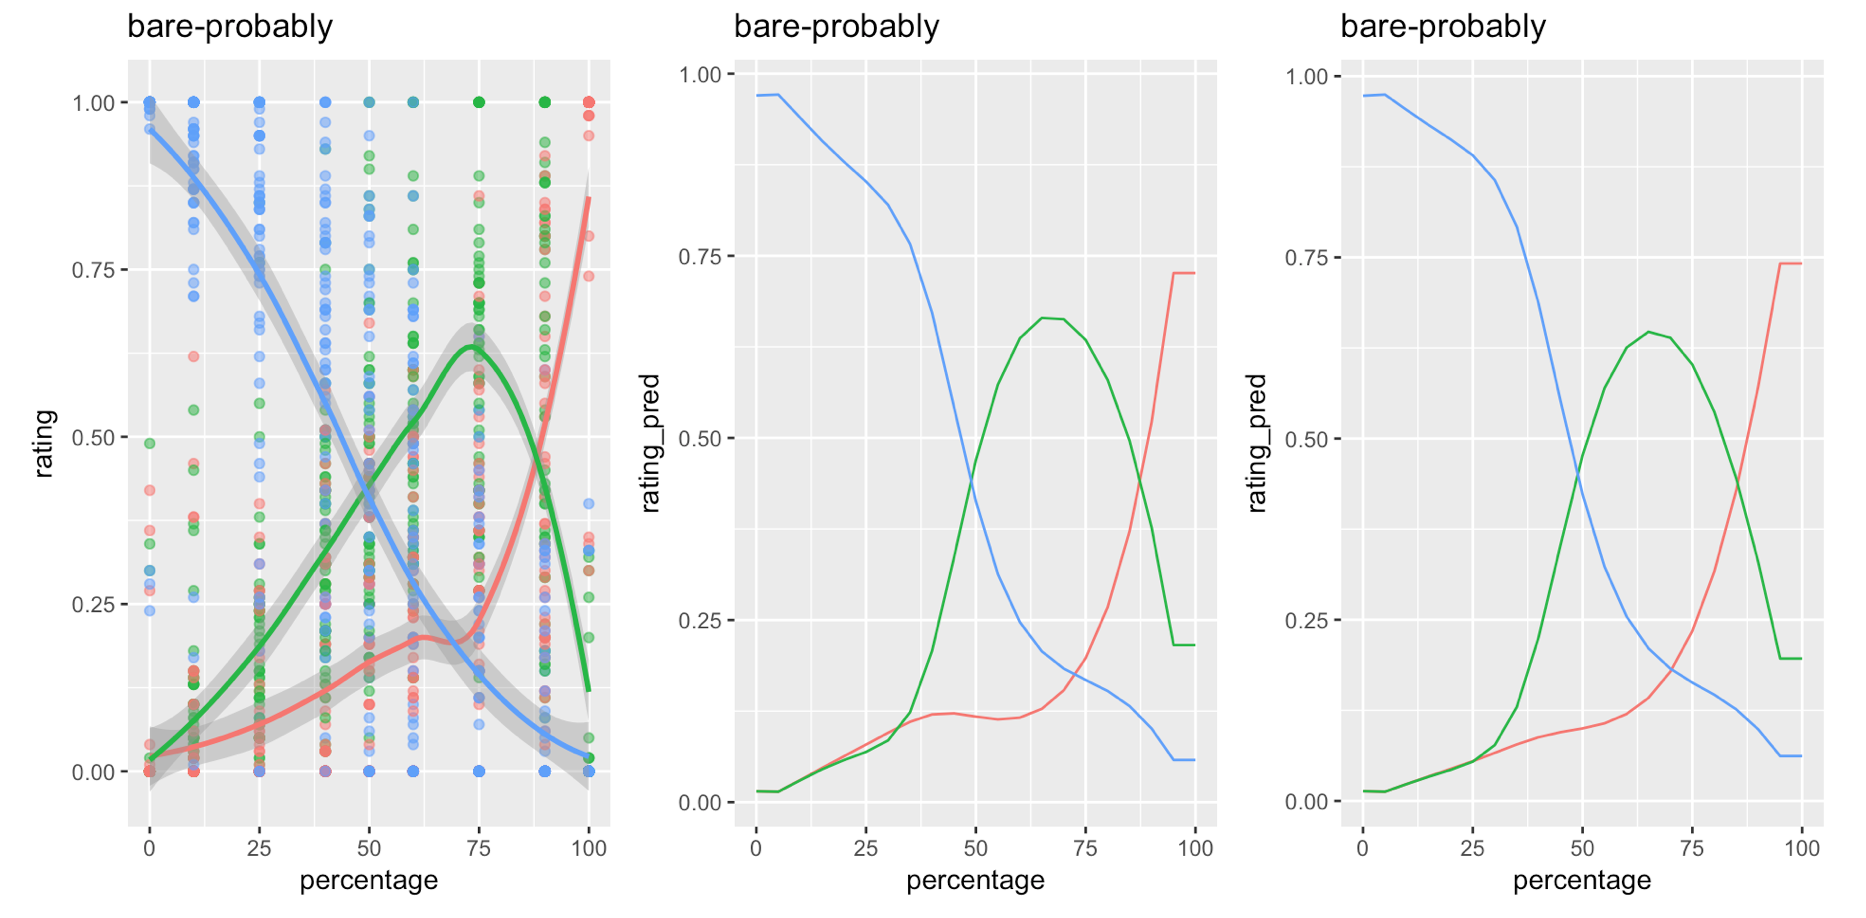
\includegraphics[width=\textwidth]{plots/bare-probably-predictions.png} \\
%bare (red) - probably (green) condition
%
%\vspace{2em}
%
%
%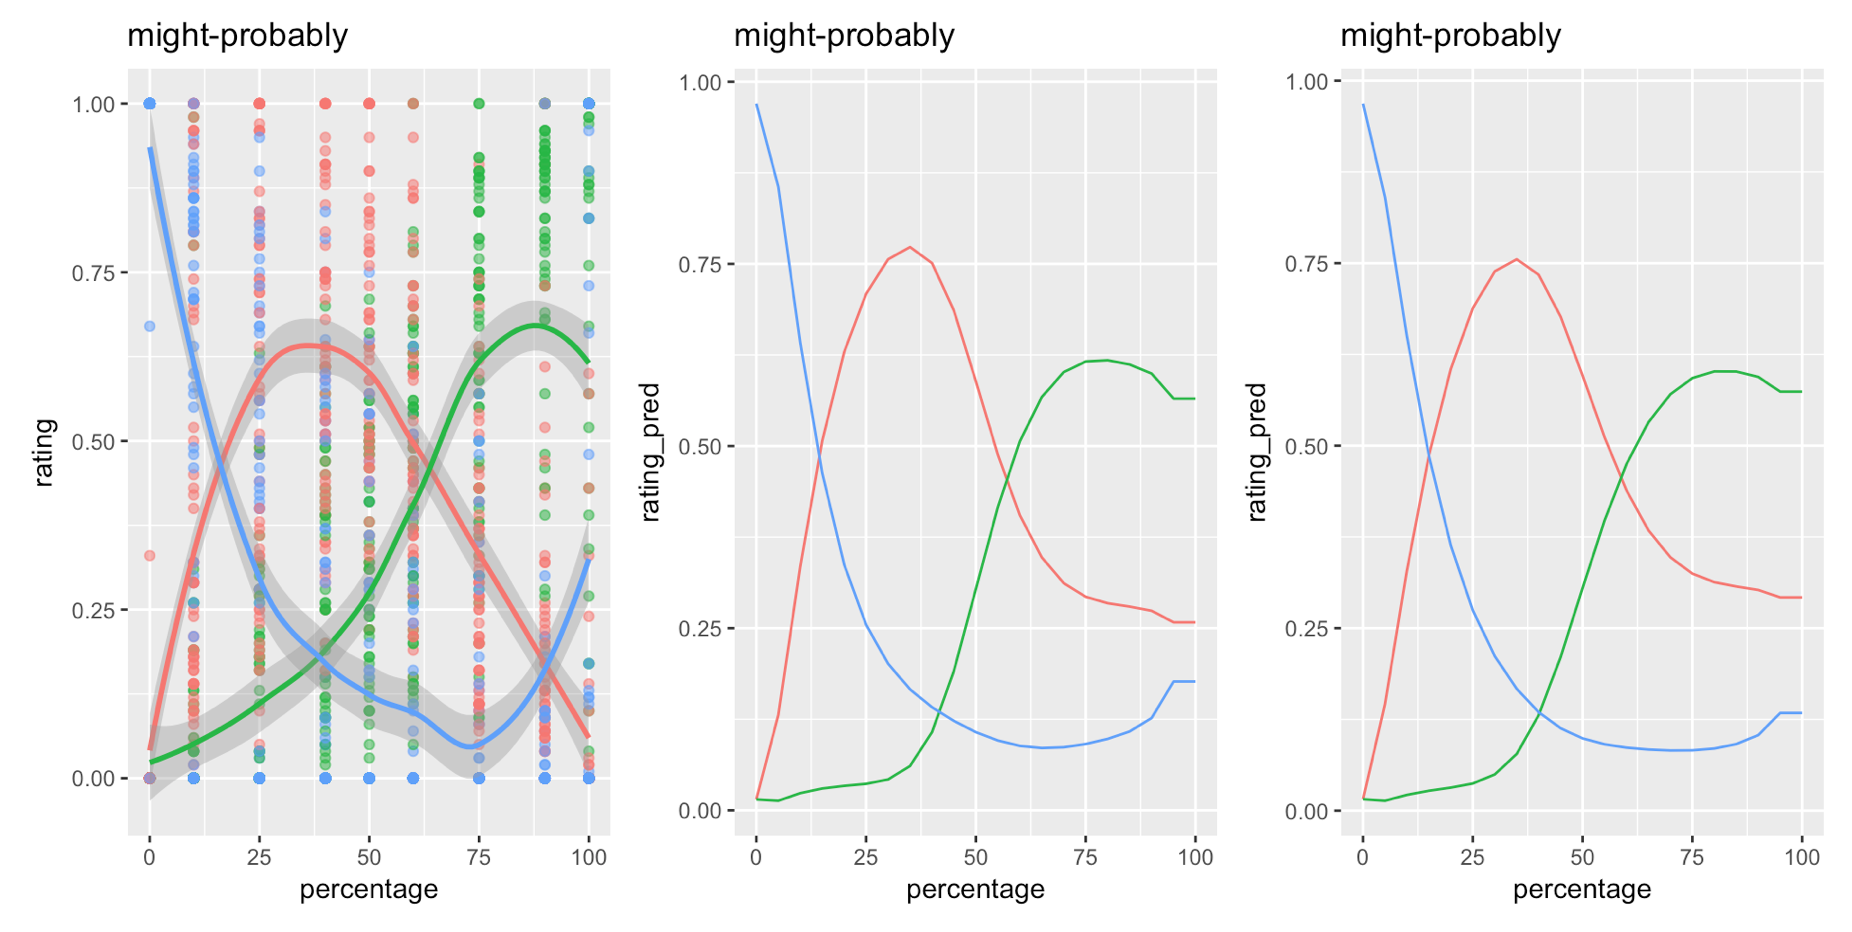
\includegraphics[width=\textwidth]{plots/might-probably-predictions.png}
%
%might (red) - probably (green) condition
%
%\vspace{2em}
%
%
%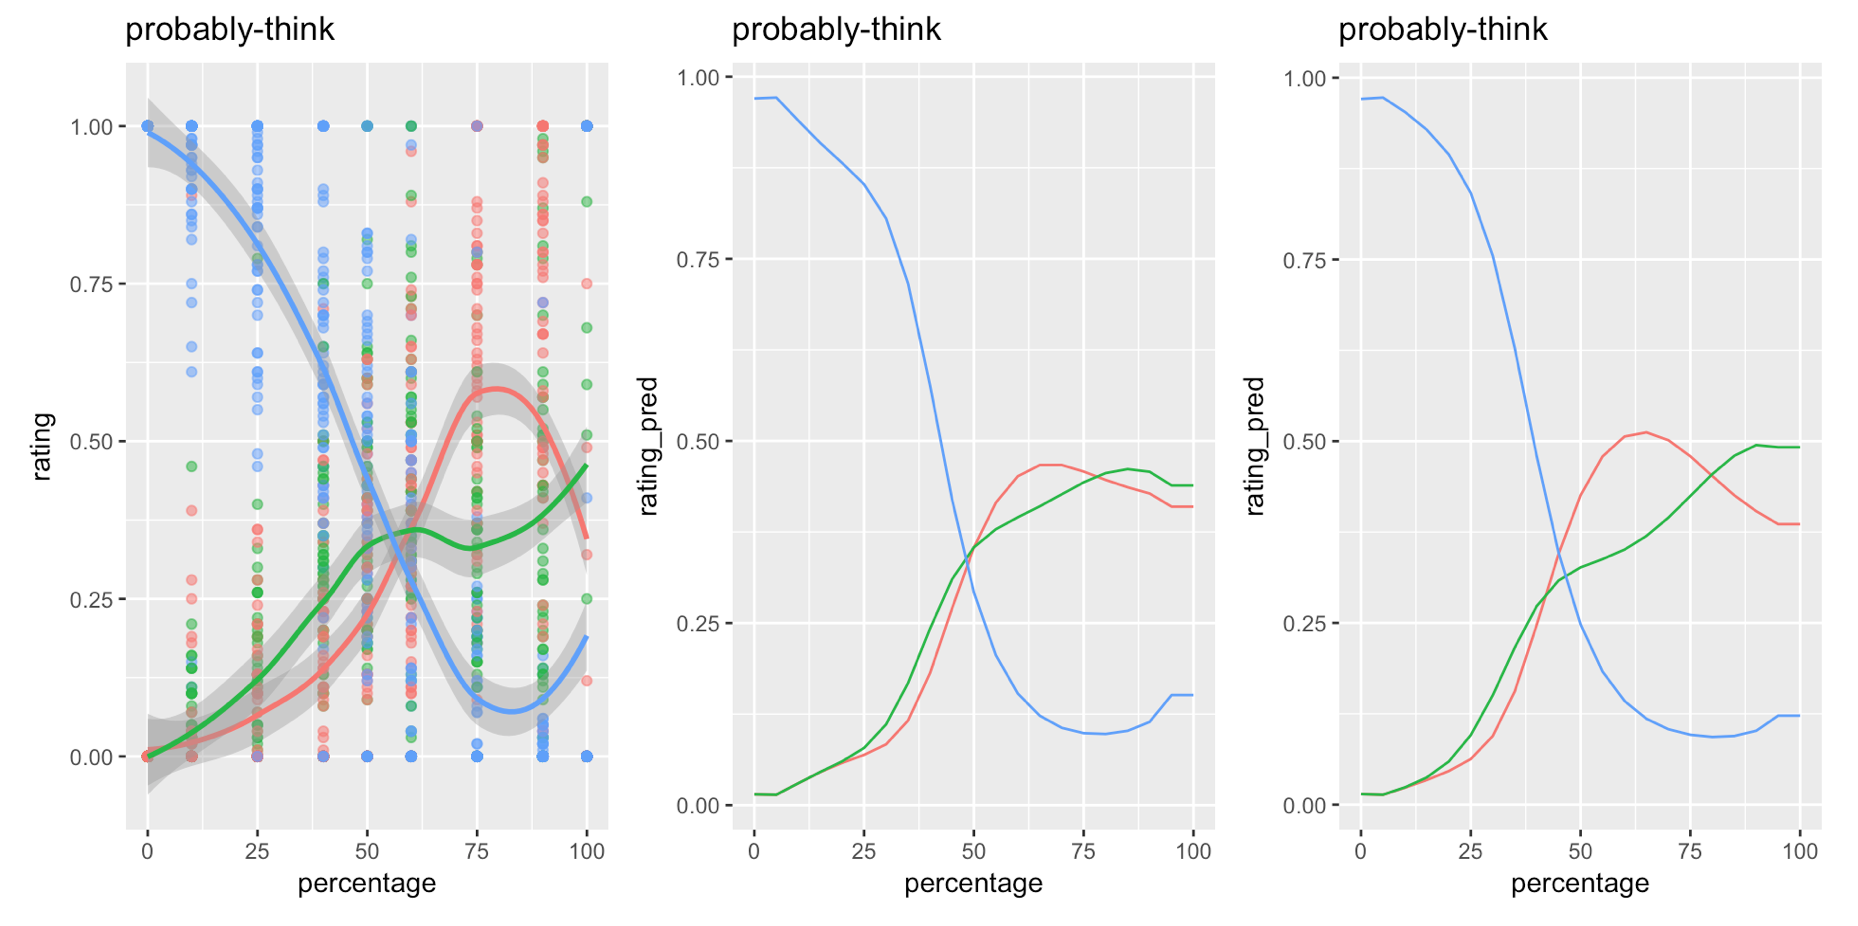
\includegraphics[width=\textwidth]{plots/probably-think-predictions.png}
%
%probably (red) - think (green) condition
%
%\vspace{2em}
%
%
%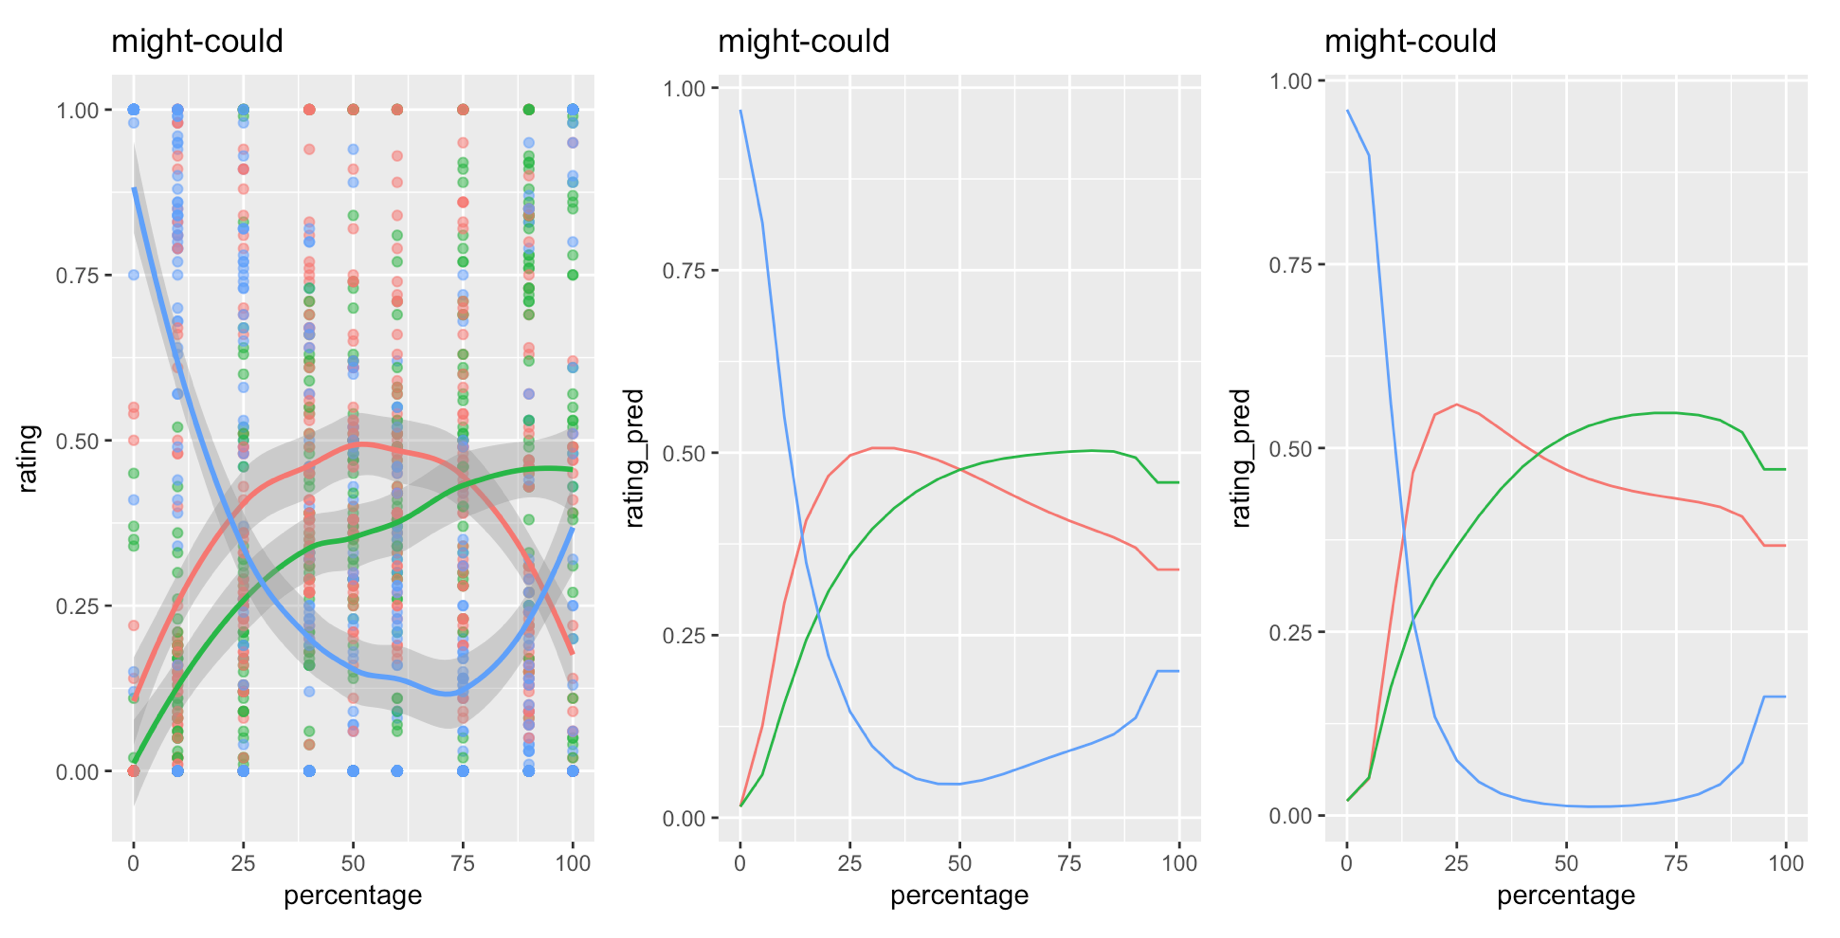
\includegraphics[width=\textwidth]{plots/might-could-predictions.png}
%
%might (red) - could (green) condition
%
%\vspace{2em}
%
%
%\end{center}
%
%In general, the model predicts the average participant responses very well -- in particular in cases in which there are clear contrasts between the utterances (e.g., here in the bare-might, bare-probably, and might-probably conditions). When the two utterances can be used for similar probability ranges (e.g., in the probably-think and the might-could condition), the model deviates a bit more from the experimental data (presumably because there are no clear differences between these two utterances in this context). A second issue with the model seems to be that in some conditions, participants seem to be more rational than the model estimates would suggest. For example, in the might-probably condition, the empirical ratings for \textit{probably} are higher than the predicted ratings.
%
%We also validated our model through cross-validation. In the above figures, the right-most plot shows the model predictions if we estimate model parameters on all conditions except for the one that we are predicting. For example, the right plot for the bare-might condition shows the predictions for this condition if we estimate the parameters using the experimental data from the 14 other conditions. Overall, the predictions with the held-out training data are almost as good as the predictions of the model trained on all the data, which suggests that this is reasonable model for predicting participant's behavior.
%
%One of the advantages of explicitly modeling participants' behavior as a Bayesian model is that we can also inspect the individual parameters, such as the distributions over thresholds $P(\theta_u)$. The following six plots show the estimated $P(\theta_u)$ for the six utterances that we included in our experiments.
%
%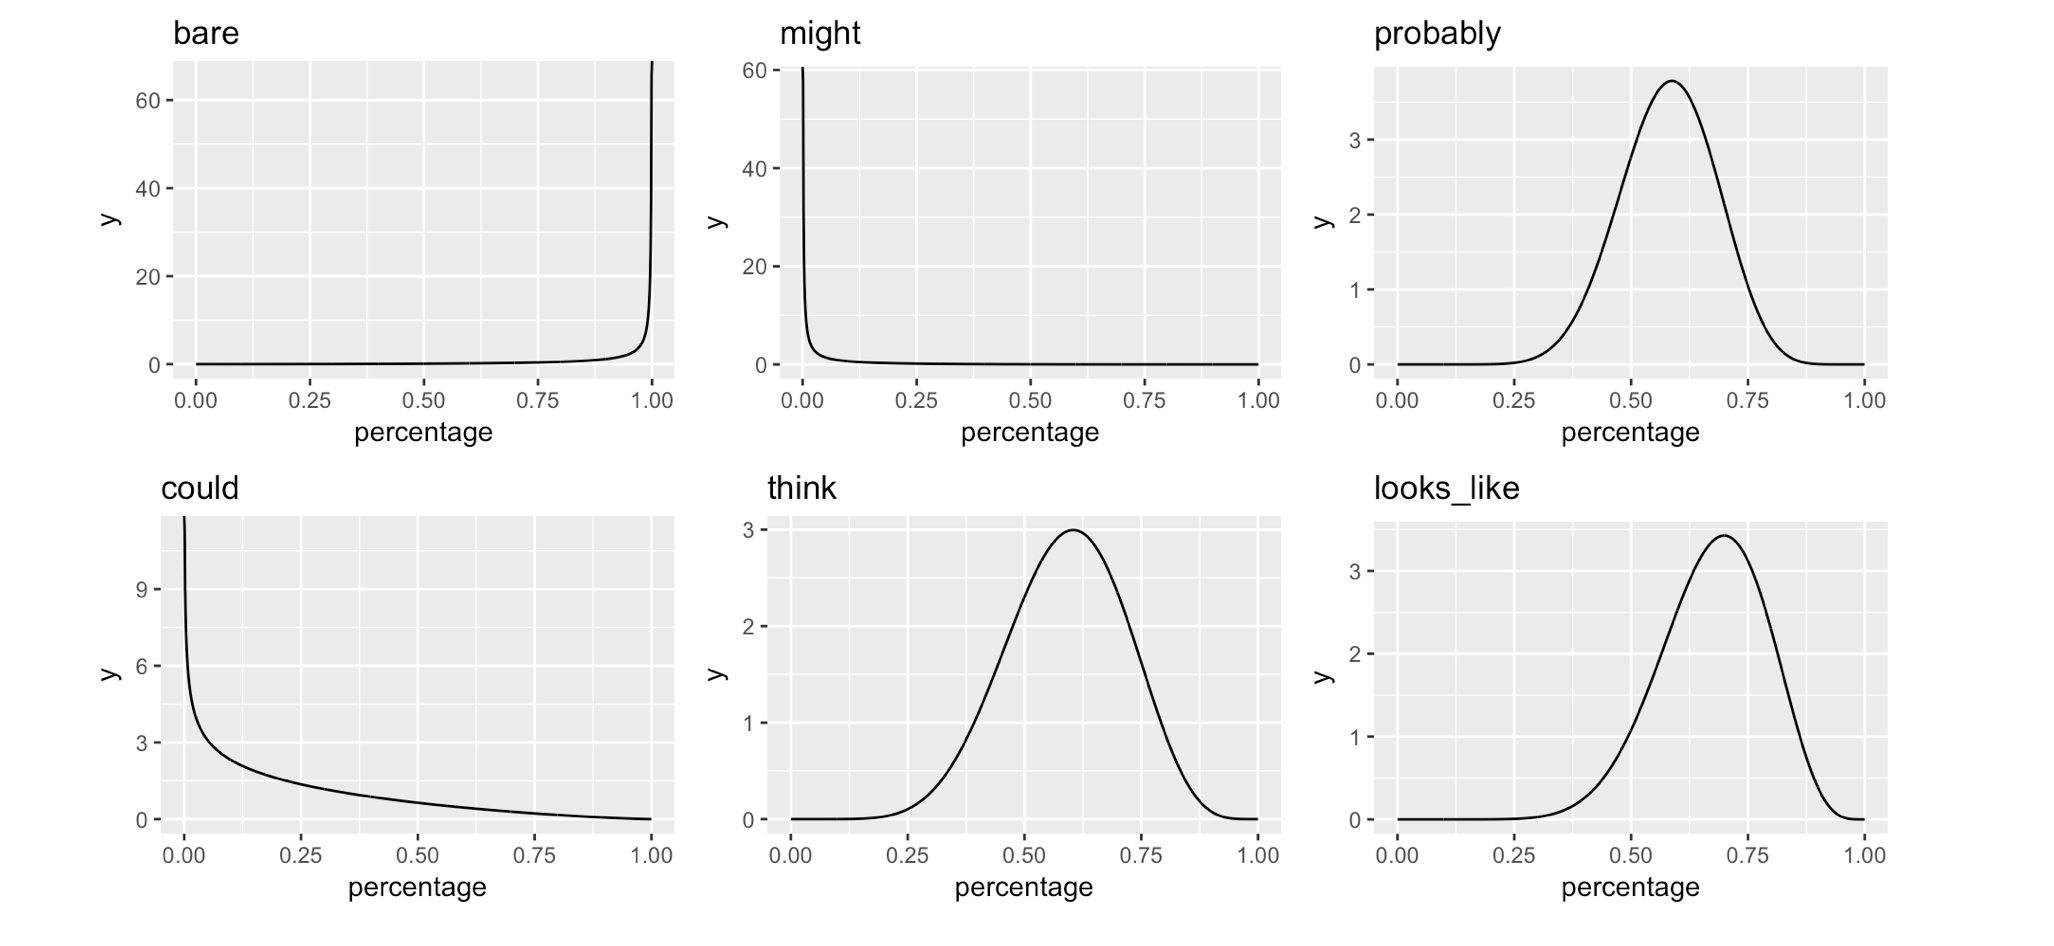
\includegraphics[width=\textwidth]{plots/threshold-distrs.png}
%
%\vspace{2em}
%
%Qualitatively, these estimated distributions are very much in line with semantic theories of modals (e.g., Kratzer (1991)): The  distributions for the thresholds for the possibility  modals \textit{might} and \textit{could} assign most of the probability mass to values slightly above 0; for bare statements most of the probability mass is close to 1 and for \textit{probably}, most of the probability mass is slightly above 0.5. The other two expressions, \textit{think} and \textit{looks like}, have--at least in this context--similar meanings as \textit{probably}. Furthermore, these results are also in line with recent experimental results by Pogue and Tanenhaus (submitted), who explicitly asked participants to rate how much certainty a speaker using these expressions conveyed.
%
%
%
%
%\subsection{Adaptation model}
%
%\subsubsection{Model and estimation}
%
%We model the adaptation process as participants  a) gaining certainty about the threshold distribution that a speaker uses and b) updating the cost parameters for the individual utterances. Our main interest is in how participants update their beliefs about the thresholds for a given speaker but considering that the speaker in the exposure trials only uses \textit{might}, \textit{probably} and bare utterances, the exposure phase also suggests to participants that the speaker has a preference for these utterances over other utterances, which we can explicitly model by allowing the adaptation model to change the cost terms for different utterances. For the exposure phase, we assume that the cost of an utterance is always $c_u$ because are not presented with alternative utterances.
%
%\vspace{1em}
%
%\textbf{Q:} Is this a reasonable argument for/the right way of changing the cost structure during the exposure phase?
%
%\vspace{1em}
%
%
%We assume that participants are doing Bayesian belief updates when they observe utterances during the exposure trials (similarly as Qing (2014) for his model of quantifier adaptation).
%
%\begin{align*}
%P(\theta, c \mid \mathscr{D}) &\propto P(\theta, c) P(\mathscr{D} \mid c, \theta)  \\
%& = P(\theta, c) \prod_{d \in \mathscr{D}} P_S(u_d \mid \phi_d; c, \theta)
%\end{align*}
%
%For the priors over thresholds $P(\theta_u)$, we take the priors that we estimated from the pre-test experimental data. For the costs, we sample from a normal distribution with $\mu=c_u$ (also estimated from the pre-test experimental data) and $\sigma=2$. The data  $\mathscr{D}$ are the 20 utterances that participants hear during the exposure phase. 
%
%\subsubsection{Model predictions}
%
%
%Participants performed the same task as in the \textit{might-probably} condition of the pre-test experiment after the exposure phase. We use the same model as in the pre-test experiment to predict participants' ratings for the utterances \textit{might} and \textit{probably} except that we are using the updated cost parameters and priors over thresholds. We use the same cost function as in the pre-test experiment, i.e., we assume that the cost for the two given utterances \textit{might} and \textit{probably} is 0.
%
%The following plots compare the post-exposure experimental results to the predicted ratings of the model for the two adaptation conditions.
%
%
%\begin{center}
%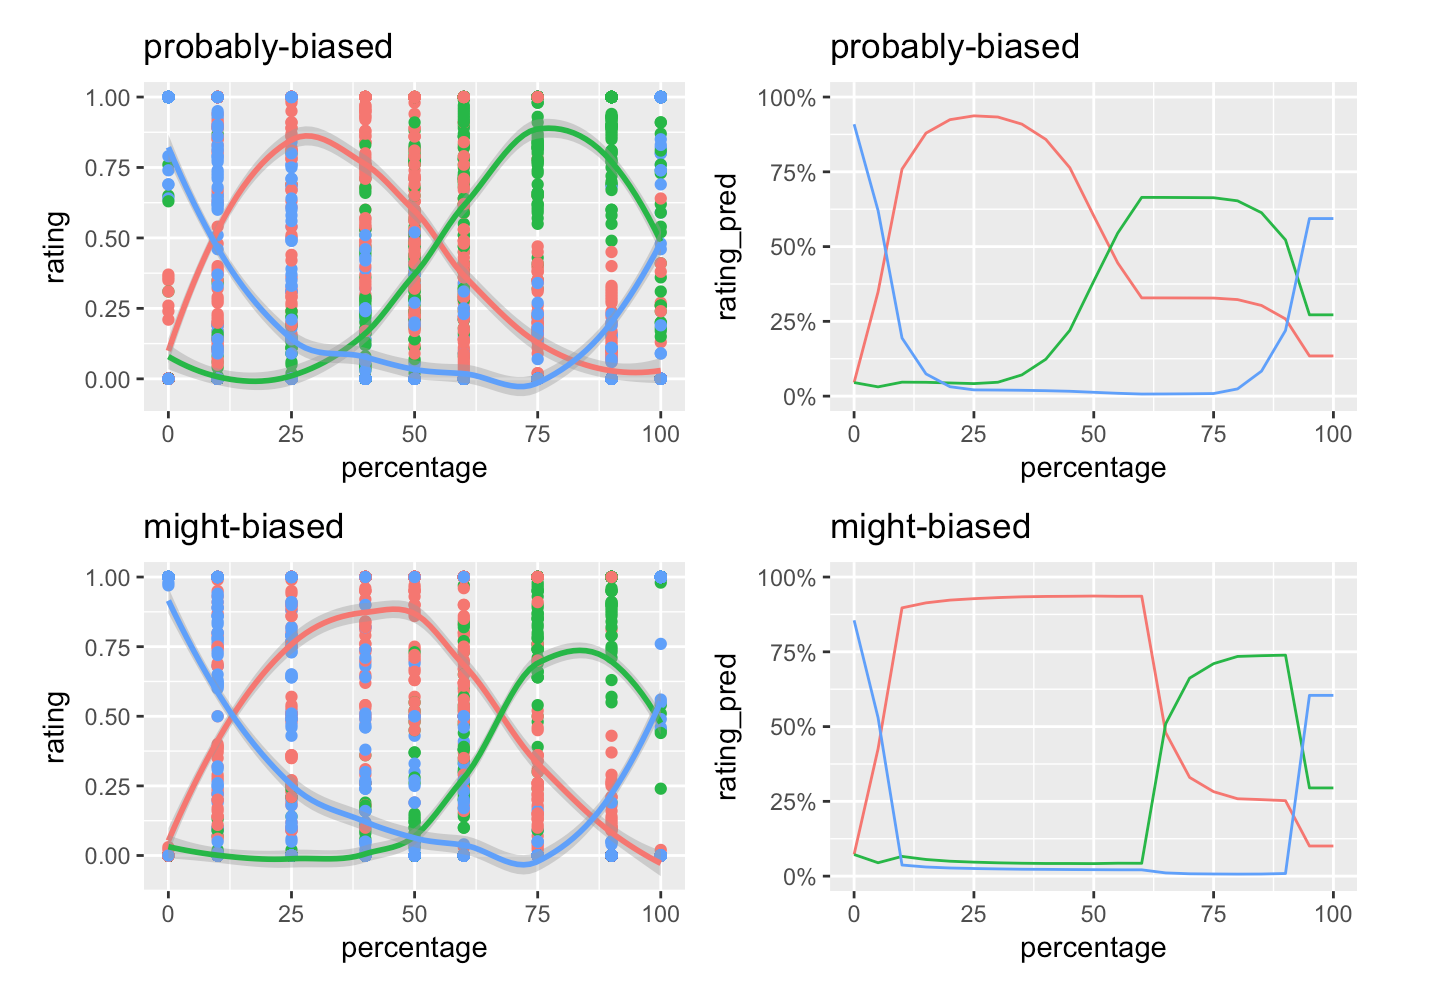
\includegraphics[width=\textwidth]{plots/adaptation-results.png}
%
%Experimental and predicted ratings for might (red), probably (green) and other (blue) for participants in the two adaptation conditions.
%
%\vspace{2em}
%\end{center}
%
%As these figures show, the model matches more or less the experimental results. In the probably-biased condition the model predicts that the curves cross at around 55\% of blue gumballs, which is what we observed in the data and similarly, the predicted and the actual point of intersection of the two curves in the might-biased condition are at around 65\%. However, the issue of too low ratings for \textit{probably} and the bare utterances that we already observed in the pre-test experiment, seems to be even stronger here. This effect could be lowered by increasing the rationality parameter $\lambda$ but it is not clear why people would be more rational in the adaptation experiment than they were in the pre-test experiment.
%
%Alternatively, we could consider using a different literal listener which does not assign a uniform probability to all event probabilities $\phi$ if they are above $\theta_u$. But again, it is unclear what these distributions would look like.
%
%As in the pre-test experiment, we can again look at the posterior distribution of $P(\theta)$ and the cost parameters for the two conditions.
%
%
%\begin{center}
%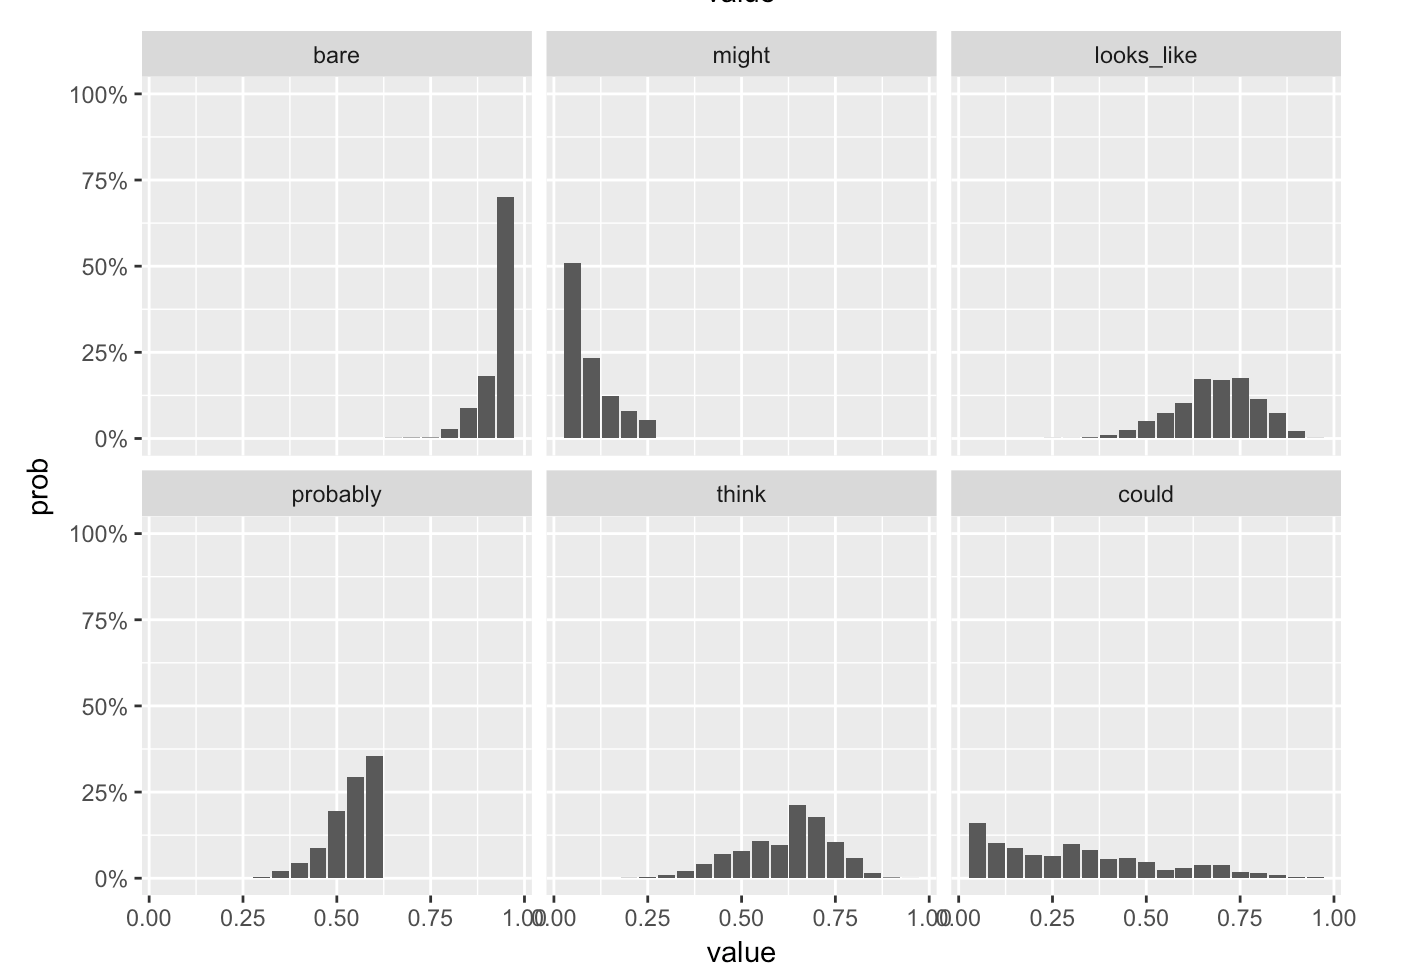
\includegraphics[width=0.9\textwidth]{plots/probably-biased-threshold-posterior.png}
%
%Posterior distributions over threshold parameters $\theta$ in the \textbf{probably-biased} condition.
%\end{center}
%
%\begin{center}
%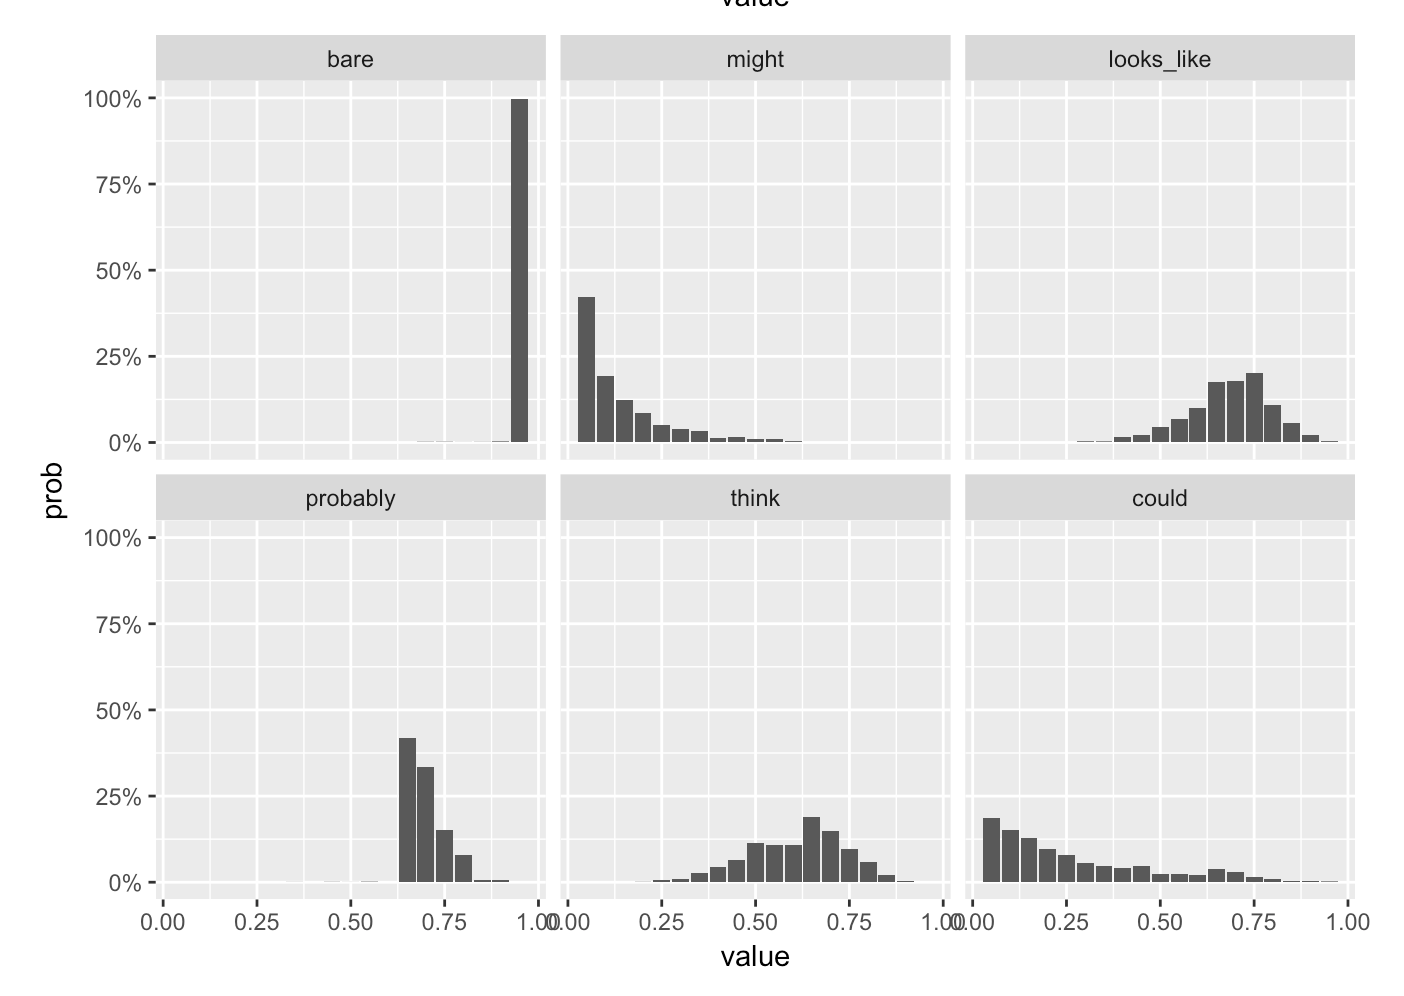
\includegraphics[width=0.9\textwidth]{plots/might-biased-threshold-posterior.png}
%
%Posterior distributions over threshold parameters $\theta$ in the \textbf{might-biased} condition.
%\vspace{2em}
%\end{center}
%
%These plots suggest that the distributions over thresholds for the three utterances that do not appear in the exposure phase remain fairly broad and match to a large extent the prior distributions.
%This suggests that participants are not updating their beliefs about the use of these expressions, which is expected given that they do not see any evidence for the use of these expressions. 
%
%\vspace{1em}
%\textbf{Note:} Would be interesting to collect post-exposure ratings for e.g., the pair \textit{could} and \textit{looks like} and see if these things remain more or less unchanged.
%\vspace{1em}
%
%The distributions over thresholds for bare utterances, \textit{might} and \textit{probably}, on the other hand, differ considerably across the two conditions and are overall much narrower. In the \textit{probably-biased} condition, 
%the model infers that the threshold should be at or slightly below 60\%, and the threshold for \textit{might} should be somewhere between 5 and 25\%.
%
%In the \textit{might-biased} condition, the distribution of $\theta_{might}$ has a slightly longer tail but overall still assumes that the threshold is low.  The distribution of $\theta_{probably}$ in this condition, is shifted to the right with the most likely threshold being at 65\% and given that the speaker in this condition always uses \textit{probably} to refer to events which are 90\% likely to happen, the distribution for $\theta_{bare}$ is also shifted to the right and much narrower. 
%
%Overall, these thresholds seem very reasonable and what is noteworthy is that the model still assigns a high probability to utterances with \textit{might} to describe events whose probability of happening is low despite the fact that participants only observe \textit{might} being used to describe  events with a probability of happening of 60\%.


%\section{Future directions/TODOs}
%
%{\bf Short-term things:}
%
%\begin{itemize}
%\item The bootstrapping procedure to estimate the variance of all $\Theta_S$ parameters potentially leads to too high estimates for the variance. One should try to turn this into a hierarchical model which puts a prior on the overall variance.
%\item We assume right now that the comprehension model should be an $L_1$ and the production model should be an $S_1$. One could also imagine that the production model should be an $S_2$. Investigate this hypothesis (in particular in light of the newly collected comprehension norming study.)
%\item Try estimating the means and variance of the hierarchical model for the Beta distributions using the mean and $nu$ parameterization -- potentially more stable than $\alpha/\beta$ parameterization.
%\item Run experiment with equal number of {\sc might} and {\sc probably} utterances to rule out only priming.
%\item Figure out if there is a way to include an ``adaptation rate''  parameter, similar to Roettger and Franke (unpublished)
%\item Try to investigate whether it's actually linguistic adaptation or rather inference of some higher-level goal (e.g., not wanting to upset the girl).
%\end{itemize}
%
%{\bf Long-term things:}
%\begin{itemize}
%\item Run experiments with multiple speakers.
%\item Run post-exposure phase with utterances that were not part in exposure (e.g., \emph{could}, \emph{looks like}). What changes about these? What does the model predict?
%\item Run experiment where the speaker uses semantically very similar items (e.g., \emph{probably} and \emph{think}) differently. Do participants also learn these differences?
%\item Run norming study  -- exposure -- prior elicitation -- production post-exposure -- comprehension post-exposure -- to verify model on individual participant level.
%\item Implement hierarchical model which can explain adaptation to multiple speakers.
%\item Consider adaptation to speakers with accents -- one potential way to model this would be to model these speakers as having more noise. This would predict that people rely more on their priors and adapt slower. (Also compare this to Gibson et al. (2017).)
%\item Consider generalizations of adaptation: Does adapting to one female speaker skew expectations more to other female speaker than to other male speaker? And vice versa? What about accents? Is this at all a function of similarity in speech (e.g., as discussed in Kraljic (2015) or Johnson (2006)).
%\item come up with paradigm where people only get indirect feedback (i.e, did something happen or not, maybe some betting game).
%
%\end{itemize}



\end{document}
